% Options for packages loaded elsewhere
\PassOptionsToPackage{unicode}{hyperref}
\PassOptionsToPackage{hyphens}{url}
\PassOptionsToPackage{dvipsnames,svgnames,x11names}{xcolor}
%
\documentclass[
  letterpaper,
  DIV=11,
  numbers=noendperiod]{scrartcl}

\usepackage{amsmath,amssymb}
\usepackage{iftex}
\ifPDFTeX
  \usepackage[T1]{fontenc}
  \usepackage[utf8]{inputenc}
  \usepackage{textcomp} % provide euro and other symbols
\else % if luatex or xetex
  \usepackage{unicode-math}
  \defaultfontfeatures{Scale=MatchLowercase}
  \defaultfontfeatures[\rmfamily]{Ligatures=TeX,Scale=1}
\fi
\usepackage{lmodern}
\ifPDFTeX\else  
    % xetex/luatex font selection
\fi
% Use upquote if available, for straight quotes in verbatim environments
\IfFileExists{upquote.sty}{\usepackage{upquote}}{}
\IfFileExists{microtype.sty}{% use microtype if available
  \usepackage[]{microtype}
  \UseMicrotypeSet[protrusion]{basicmath} % disable protrusion for tt fonts
}{}
\makeatletter
\@ifundefined{KOMAClassName}{% if non-KOMA class
  \IfFileExists{parskip.sty}{%
    \usepackage{parskip}
  }{% else
    \setlength{\parindent}{0pt}
    \setlength{\parskip}{6pt plus 2pt minus 1pt}}
}{% if KOMA class
  \KOMAoptions{parskip=half}}
\makeatother
\usepackage{xcolor}
\setlength{\emergencystretch}{3em} % prevent overfull lines
\setcounter{secnumdepth}{5}
% Make \paragraph and \subparagraph free-standing
\ifx\paragraph\undefined\else
  \let\oldparagraph\paragraph
  \renewcommand{\paragraph}[1]{\oldparagraph{#1}\mbox{}}
\fi
\ifx\subparagraph\undefined\else
  \let\oldsubparagraph\subparagraph
  \renewcommand{\subparagraph}[1]{\oldsubparagraph{#1}\mbox{}}
\fi


\providecommand{\tightlist}{%
  \setlength{\itemsep}{0pt}\setlength{\parskip}{0pt}}\usepackage{longtable,booktabs,array}
\usepackage{calc} % for calculating minipage widths
% Correct order of tables after \paragraph or \subparagraph
\usepackage{etoolbox}
\makeatletter
\patchcmd\longtable{\par}{\if@noskipsec\mbox{}\fi\par}{}{}
\makeatother
% Allow footnotes in longtable head/foot
\IfFileExists{footnotehyper.sty}{\usepackage{footnotehyper}}{\usepackage{footnote}}
\makesavenoteenv{longtable}
\usepackage{graphicx}
\makeatletter
\def\maxwidth{\ifdim\Gin@nat@width>\linewidth\linewidth\else\Gin@nat@width\fi}
\def\maxheight{\ifdim\Gin@nat@height>\textheight\textheight\else\Gin@nat@height\fi}
\makeatother
% Scale images if necessary, so that they will not overflow the page
% margins by default, and it is still possible to overwrite the defaults
% using explicit options in \includegraphics[width, height, ...]{}
\setkeys{Gin}{width=\maxwidth,height=\maxheight,keepaspectratio}
% Set default figure placement to htbp
\makeatletter
\def\fps@figure{htbp}
\makeatother

\usepackage{booktabs}
\usepackage{longtable}
\usepackage{array}
\usepackage{multirow}
\usepackage{wrapfig}
\usepackage{float}
\usepackage{colortbl}
\usepackage{pdflscape}
\usepackage{tabu}
\usepackage{threeparttable}
\usepackage{threeparttablex}
\usepackage[normalem]{ulem}
\usepackage{makecell}
\usepackage{xcolor}
\KOMAoption{captions}{tableheading}
\makeatletter
\@ifpackageloaded{caption}{}{\usepackage{caption}}
\AtBeginDocument{%
\ifdefined\contentsname
  \renewcommand*\contentsname{Table of contents}
\else
  \newcommand\contentsname{Table of contents}
\fi
\ifdefined\listfigurename
  \renewcommand*\listfigurename{List of Figures}
\else
  \newcommand\listfigurename{List of Figures}
\fi
\ifdefined\listtablename
  \renewcommand*\listtablename{List of Tables}
\else
  \newcommand\listtablename{List of Tables}
\fi
\ifdefined\figurename
  \renewcommand*\figurename{Figure}
\else
  \newcommand\figurename{Figure}
\fi
\ifdefined\tablename
  \renewcommand*\tablename{Table}
\else
  \newcommand\tablename{Table}
\fi
}
\@ifpackageloaded{float}{}{\usepackage{float}}
\floatstyle{ruled}
\@ifundefined{c@chapter}{\newfloat{codelisting}{h}{lop}}{\newfloat{codelisting}{h}{lop}[chapter]}
\floatname{codelisting}{Listing}
\newcommand*\listoflistings{\listof{codelisting}{List of Listings}}
\makeatother
\makeatletter
\makeatother
\makeatletter
\@ifpackageloaded{caption}{}{\usepackage{caption}}
\@ifpackageloaded{subcaption}{}{\usepackage{subcaption}}
\makeatother
\ifLuaTeX
  \usepackage{selnolig}  % disable illegal ligatures
\fi
\usepackage{bookmark}

\IfFileExists{xurl.sty}{\usepackage{xurl}}{} % add URL line breaks if available
\urlstyle{same} % disable monospaced font for URLs
\hypersetup{
  pdftitle={Samlede notater},
  colorlinks=true,
  linkcolor={blue},
  filecolor={Maroon},
  citecolor={Blue},
  urlcolor={Blue},
  pdfcreator={LaTeX via pandoc}}

\title{Samlede notater}
\author{}
\date{}

\begin{document}
\maketitle

\renewcommand*\contentsname{Table of contents}
{
\hypersetup{linkcolor=}
\setcounter{tocdepth}{3}
\tableofcontents
}
\listoffigures
\listoftables
\section{Kapittel 1: Introduksjon til mikroøkonomi. Overblikk over
fulllkomen
konkurranse}\label{kapittel-1-introduksjon-til-mikrouxf8konomi.-overblikk-over-fulllkomen-konkurranse}

\begin{center}\rule{0.5\linewidth}{0.5pt}\end{center}

\subsection{Hva handler økonomi om?}\label{hva-handler-uxf8konomi-om}

\begin{itemize}
\tightlist
\item
  Hva handler økonomi om?
\item
  Mikroøkonomi er en del av samfunnsøkonomi. Hvilke temaer forbinder du
  med samfunnsøkonomi?
\item
  En kort historie om en tur i butikken.

  \begin{itemize}
  \tightlist
  \item
    Hvilke varer skal du kjøpe?
  \item
    Hvor mye skal du kjøpe av de ulike varene?
  \end{itemize}
\item
  Hva har økonomi med dette å gjøre? Tre relevante forhold:

  \begin{itemize}
  \tightlist
  \item
    \begin{enumerate}
    \def\labelenumi{(\roman{enumi})}
    \tightlist
    \item
      Varene må ha blitt produsert.
    \end{enumerate}
  \item
    \begin{enumerate}
    \def\labelenumi{(\roman{enumi})}
    \setcounter{enumi}{1}
    \tightlist
    \item
      Du må tilby noe for å bytte til deg varer. Betalingsmiddel
    \end{enumerate}
  \item
    og handel.
  \item
    \begin{enumerate}
    \def\labelenumi{(\roman{enumi})}
    \setcounter{enumi}{2}
    \tightlist
    \item
      Du må ha skaffet betalingsmiddelet.
    \end{enumerate}
  \end{itemize}
\end{itemize}

\begin{center}\rule{0.5\linewidth}{0.5pt}\end{center}

\textbf{Altså \ldots{}}

\begin{itemize}
\tightlist
\item
  Selv i den «enkle» historien er det:

  \begin{itemize}
  \tightlist
  \item
    Flere beslutninger involvert.
  \item
    Flere markeder involvert.
  \end{itemize}
\item
  Men: hvorfor får vi ikke alle varer vi vil ha? Rundt oss ser vi (og
  opplever selv) stor etterspørsel.Vi trenger jo en rekke ting, også i
  Norge.

  \begin{itemize}
  \tightlist
  \item
    Svaret er: KNAPPHET!
  \end{itemize}
\end{itemize}

\begin{center}\rule{0.5\linewidth}{0.5pt}\end{center}

\subsection{Definisjon}\label{definisjon}

\begin{itemize}
\tightlist
\item
  Definisjon av økonomi:
\end{itemize}

\emph{Handler om bruken av knappe ressurser for å dekke menneskelig
behov.}

\begin{itemize}
\tightlist
\item
  Den delen av samfunnsvitenskapene som studerer de valgene som
  individer, bedrifter, myndigheter og samfunn må ta, som følge av
  knapphet.
\item
  To stikkord: behov og ressurser. Komme tilbake til\ldots{}
\item
  Bedriftsøkonomi og samfunnsøkonomi: Hvorfor skal dere lære
  samfunnsøkonomi på dette studiet? Relevant for bedrifter?
\end{itemize}

\begin{center}\rule{0.5\linewidth}{0.5pt}\end{center}

\subsection{Behov}\label{behov}

\begin{itemize}
\tightlist
\item
  Økonomers behandling av behov og behovsdannelse. For enkelt?
  Psykologers behandling av samme tema\ldots{}
\item
  Et grovt skille:

  \begin{itemize}
  \tightlist
  \item
    Som må dekkes
  \item
    Ønsker
  \end{itemize}
\item
  Behov avdekkes gjennom preferanser, som igjen kan avdekkes via
  etterspørsel.
\item
  Kan behov skapes? Jepp. Men er slike skapte behov mer eller mindre
  viktig enn ''andre'' behov, gitt knappe ressurser.
\item
  En måte å skjære gjennom denne problemstillingen på er å legge til
  grunn \emph{konsumentsuverenitet}.

  \begin{itemize}
  \tightlist
  \item
    ''Folk vet best selv hva som er best for dem''.
  \end{itemize}
\end{itemize}

\begin{center}\rule{0.5\linewidth}{0.5pt}\end{center}

\subsection{Ressurser}\label{ressurser}

\begin{itemize}
\tightlist
\item
  Innsatsfaktor eller produksjonsfaktor kan betegnes som synonyme ord.
  \(\Rightarrow\) Faktorer som er ''input'' i produksjonsprosessen.
\item
  Kategorier:

  \begin{itemize}
  \tightlist
  \item
    Naturressurser: Fornybare og ikke-fornybare
  \item
    Arbeidskraft
  \item
    Realkapital: Kan brukes direkte eller indirekte
  \end{itemize}
\item
  Ressurser som er KNAPPE.
\item
  Er penger ressurser??
\end{itemize}

\begin{center}\rule{0.5\linewidth}{0.5pt}\end{center}

\subsection{Så kjernen i økonomifaget er
dermed:}\label{suxe5-kjernen-i-uxf8konomifaget-er-dermed}

\begin{itemize}
\tightlist
\item
  Ettersom det er knapphet på ressurser kombinert med store behov, er
  det ønskelig å bruke ressursene smartest mulig. \(\Rightarrow\) Sikre
  at utnyttelsen av ressursene er optimal.
\item
  Merk at ressurser ofte har alternativ anvendelse. Dette innebærer at
  dersom vi bruker en ressurs til å produsere en vare, kan ikke den
  samme ressursen brukes samtidig til å produsere en annen vare. Av og
  til ikke i det hele tatt.
\end{itemize}

\begin{center}\rule{0.5\linewidth}{0.5pt}\end{center}

\subsection{Alternativkostnad}\label{alternativkostnad}

\begin{itemize}
\tightlist
\item
  Dette er et helt sentralt begrep i økonomifaget.
\item
  Bruk av ressurser tilfører en verdi som skal dekke menneskelige behov.
\item
  Ressurser har en alternativ anvendelse. Den beste alternative
  anvendelse har også en verdi. Denne verdien tapes når vi bruker
  ressursen til et bestemt formål.
\item
  Dette tapet er alternativkostnaden.

  \begin{itemize}
  \tightlist
  \item
    \emph{Alternativkostnaden er altså verdien av beste alternative
    anvendelse.}
  \end{itemize}
\end{itemize}

\begin{figure}[H]

{\centering 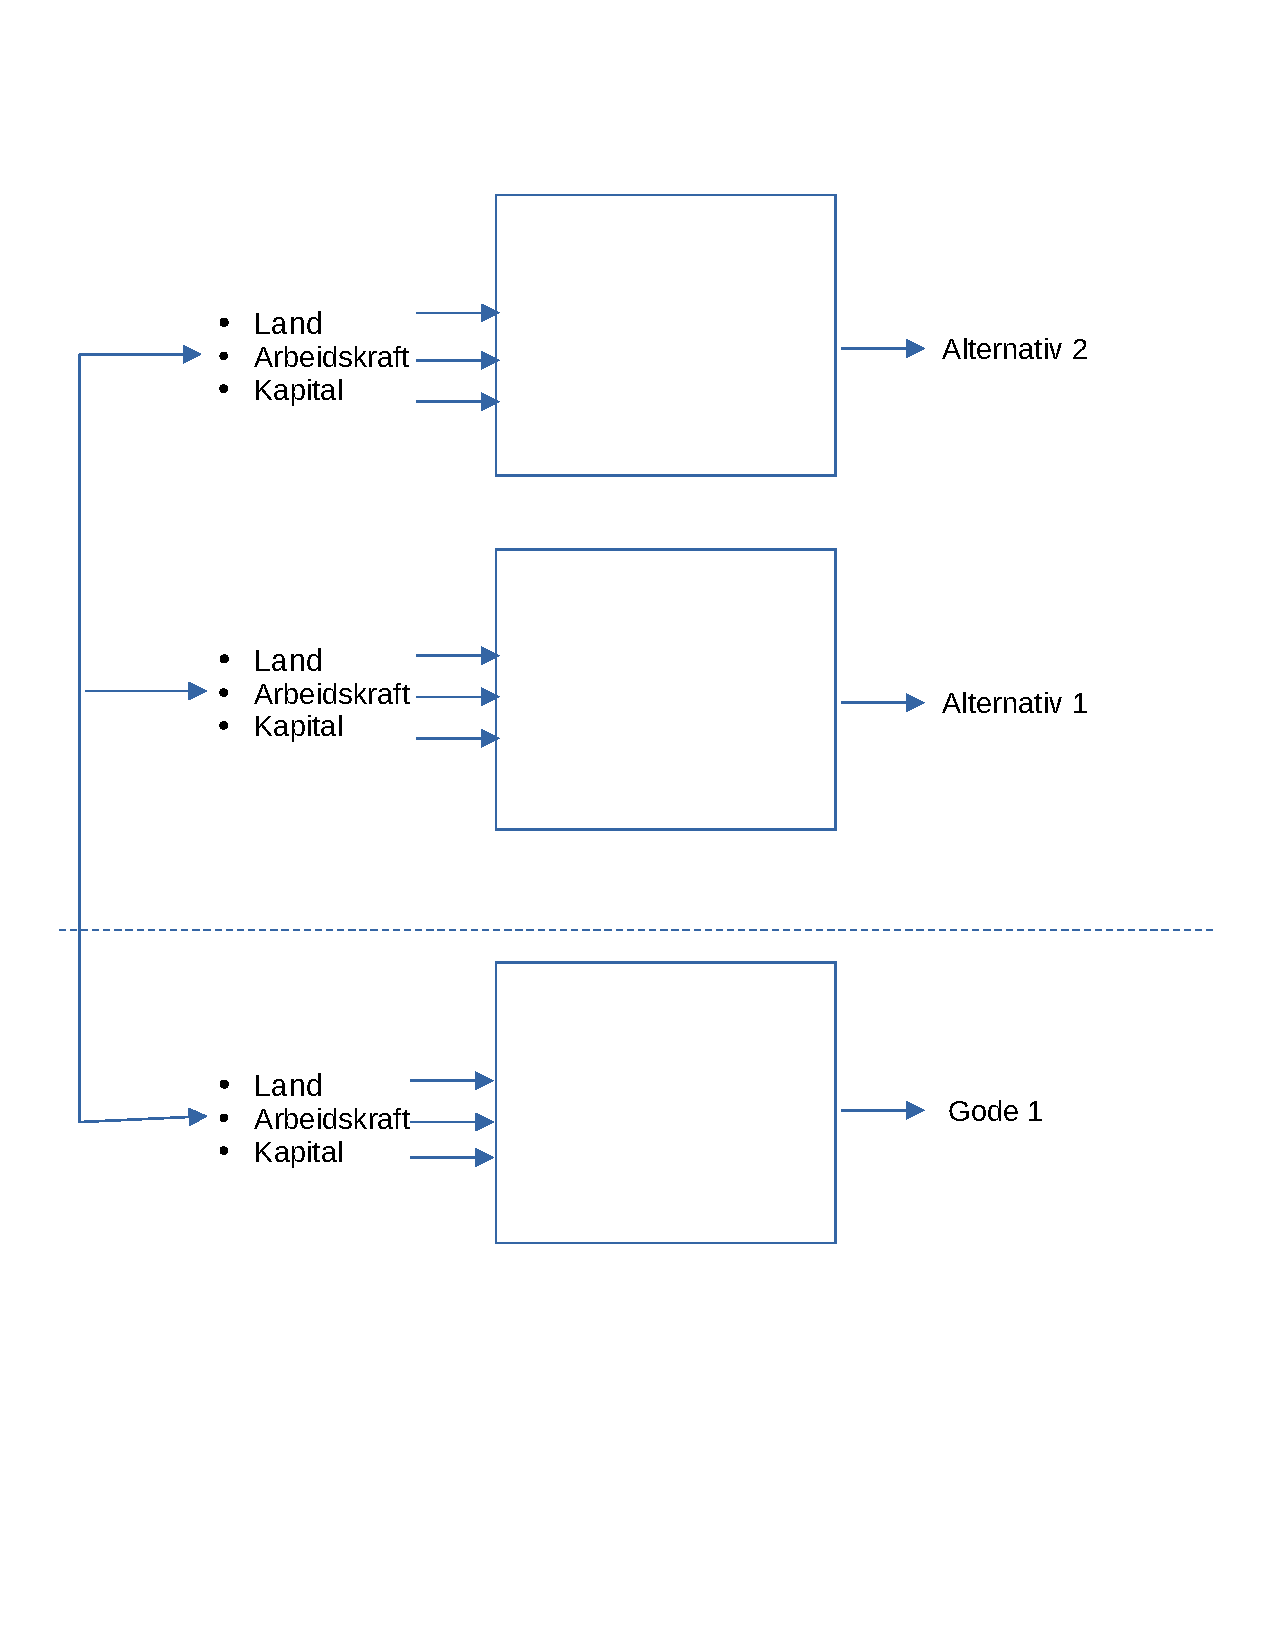
\includegraphics[width=0.5\textwidth,height=\textheight]{allenotater_files/mediabag/drawio/alternativ.pdf}

}

\caption{Figur 2.1}

\end{figure}%

\begin{center}\rule{0.5\linewidth}{0.5pt}\end{center}

\subsection{To sentrale spørsmål: spørsmål
1}\label{to-sentrale-spuxf8rsmuxe5l-spuxf8rsmuxe5l-1}

\begin{itemize}
\tightlist
\item
  (1): Hvordan vil ulike valg bestemme hvilke goder som produseres,
  hvordan de produseres og for hvem?

  \begin{itemize}
  \tightlist
  \item
    Goder skal dekke behov og ønsker.
  \item
    Men hva skal vi produsere og hvordan vet vi det?
  \item
    Hvor mye skal produseres?
  \item
    Hvordan? Vil ny teknologi erstatte arbeidskraft og føre til økt
    arbeidsledighet?
  \item
    Hvem skal det produseres til? Inntektsulikhet.
  \end{itemize}
\end{itemize}

\begin{center}\rule{0.5\linewidth}{0.5pt}\end{center}

\subsection{To sentrale spørsmål: spørsmål
2}\label{to-sentrale-spuxf8rsmuxe5l-spuxf8rsmuxe5l-2}

\begin{itemize}
\tightlist
\item
  (2): Er det slik at valg som fremmer egeninteresse også fremmer
  samfunnets beste?

  \begin{itemize}
  \tightlist
  \item
    Brukes de knappe ressursene på best mulig måte?
  \item
    Egeninteresse: valg som er best for en selv.
  \item
    Sosial interesse: valg som er best for samfunnet som helhet.
  \item
    Dine valg påvirker mange og valgene er knyttet sammen. Anta at alle
    valgene er gjort av egeninteresse, er det mulig at resultatet også
    er det beste for samfunnet som helhet?
  \item
    Adam Smith: JA. «Usynlige hånd».
  \end{itemize}
\end{itemize}

\begin{center}\rule{0.5\linewidth}{0.5pt}\end{center}

\subsection{Økonomisk tankemåte: metodologiske
tradisjoner}\label{uxf8konomisk-tankemuxe5te-metodologiske-tradisjoner}

\begin{itemize}
\tightlist
\item
  Økonomifaget defineres ut i fra tema som studeres, men det er en del
  metodiske tradisjoner.

  \begin{enumerate}
  \def\labelenumi{\arabic{enumi}.}
  \tightlist
  \item
    Et valg er en avveining (trade-off). Knapphet skaper valg.
  \item
    Kostnad: det du må gi opp.
  \item
    Fordel (benefit) eller nytte: Gleden du oppnår. Preferanser.
  \item
    Rasjonelle valg. Bruker all tilgjengelig informasjon, og veier så
    sammen kostnader og fordeler.
  \item
    Valg på marginen. Ikke enten-eller, men hvor mye. Marginalkostnad og
    marginalfordel.
  \item
    Valg responderer på incentiver. Incentiv: Belønning eller straff som
    følge av valg.
  \end{enumerate}
\end{itemize}

\begin{center}\rule{0.5\linewidth}{0.5pt}\end{center}

\subsection{Økonomi som vitenskap}\label{uxf8konomi-som-vitenskap}

\subsubsection{Modeller}\label{modeller}

\begin{itemize}
\tightlist
\item
  Bruker økonomiske modeller.
\item
  Hva er en modell? En forenklet beskrivelse av virkeligheten. Bygger
  pr. definisjon på forutsetninger.
\item
  Hvorfor bruke modeller? For å kunne fokusere på ett eller noen
  aspekter av virkeligheten. Virkeligheten er komplisert\ldots{}
\item
  Modeller gjør at vi kan rense vekk momenter som vi tror ikke har noen
  spesiell innvirkning på vårt spørsmål.
\end{itemize}

\begin{center}\rule{0.5\linewidth}{0.5pt}\end{center}

\subsubsection{Skillet mellom mikroøkonomi og
makroøkonomi}\label{skillet-mellom-mikrouxf8konomi-og-makrouxf8konomi}

\begin{itemize}
\tightlist
\item
  Det finnes flere måter å strukturere økonomifaget på. Disiplinen
  består av en rekke underområder.

  \begin{itemize}
  \tightlist
  \item
    Mikroøkonomi: Søker å forklare aktørers beslutninger, tilpasning og
    interaksjon.

    \begin{itemize}
    \tightlist
    \item
      Aktører: Bedrifter, konsumenter, markeder.
    \end{itemize}
  \item
    Makroøkonomi: Søker å studere og forklare aggregerte størrelser.
    Økonomien under ett.

    \begin{itemize}
    \tightlist
    \item
      Makroøkonomi kan deles inn i konjunkturteori og økonomisk vekst.
    \end{itemize}
  \end{itemize}
\end{itemize}

\section{Kapittel 3: En markedsmodell med fullkommen
konkurranse}\label{kapittel-3-en-markedsmodell-med-fullkommen-konkurranse}

\begin{center}\rule{0.5\linewidth}{0.5pt}\end{center}

\subsection{Innledning}\label{innledning}

\begin{itemize}
\tightlist
\item
  Bytteøkonomi og markedsøkonomi: I en markedsøkonomi (pengeøkonomi)
  byttes varer \emph{indirekte}.
\item
  Et marked består av en tilbudsside og en etterspørselsside.
\item
  Vi skal nå se på den enkleste markedsformen i økonomisk teori:
  Markedsmodell med fullkommen konkurranse
\item
  Markedsformen er likevel nyttig:

  \begin{itemize}
  \tightlist
  \item
    Selvstendig analyseapparat.
  \item
    Kan utvides langs mange dimensjoner.
  \item
    Er samfunnsøkonomisk effektiv (hva som menes med dette skal vi bruke
    litt tid på nå, men mere tid på senere).
  \item
    Er en referansemodell som andre modeller og resultater kan
    sammenlignes mot.
  \end{itemize}
\end{itemize}

\begin{center}\rule{0.5\linewidth}{0.5pt}\end{center}

\subsection{Bakgrunn}\label{bakgrunn}

\begin{itemize}
\tightlist
\item
  Store deler av kurset vil handle om teorien bak denne modellen. MERK
  at oppbyggingen gir oss flere selvstendige modeller som er nyttige for
  økonomiske analyser.
\item
  Modellen går langt tilbake:

  \begin{itemize}
  \tightlist
  \item
    Adam Smith (1723-1790) \(\rightarrow\)
  \item
    Nyklassikerne og John Stuart Mill (1806-1873) \(\rightarrow\)
  \item
    Alfred Marshall (1842-1924) \(\rightarrow\)
  \item
    Paul Samuelson (1915-2009) mfl.
  \end{itemize}
\item
  Vi skal komme tilbake til forutsetningene bak denne modellen i
  kapittel 9.
\item
  Men merk spesielt: Aktørene er \emph{pristakere} og har ingen
  innflytelse på pris som enkeltaktør, men \emph{summen} av aktørenes
  adferd bestemmer markedsprisen.
\end{itemize}

\begin{center}\rule{0.5\linewidth}{0.5pt}\end{center}

\subsection{Markedsetterspørsel}\label{markedsetterspuxf8rsel}

\begin{itemize}
\tightlist
\item
  Etterspørsel etter varer og tjenester. Ofte kalles varer + tjenester
  for goder.
\item
  Hva bestemmer etterspørselen? Priser, inntekt med mer.
\item
  Etterspørselsloven:

  \begin{itemize}
  \tightlist
  \item
    Økt pris \(\rightarrow\) lavere etterspørsel, alt annet konstant
    (cet.par.).
  \item
    Flere forhold holdes her konstante. Vi ser kun på endringer i prisen
    på varen. En endring i denne vil flytte oss langs kurven.
  \item
    En endring i konstantene vil føre til skift i kurven.
  \end{itemize}
\item
  Fra et individs etterspørsel til markedsetterspørsel.
\end{itemize}

\begin{figure}[H]

{\centering 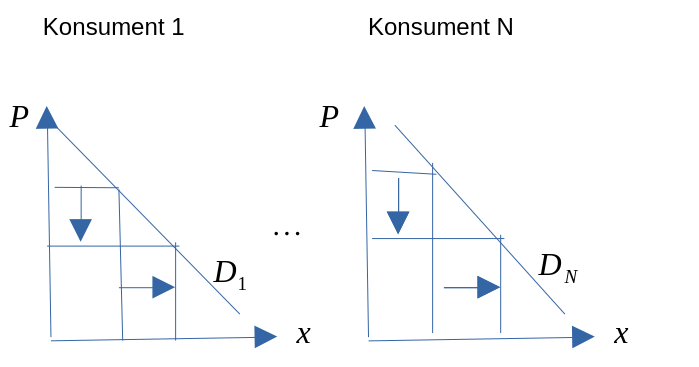
\includegraphics[width=0.65\textwidth,height=\textheight]{drawio/ekurve.png}

}

\caption{Figur 3.1}

\end{figure}%

\begin{center}\rule{0.5\linewidth}{0.5pt}\end{center}

\subsection{Markedstilbud}\label{markedstilbud}

\begin{itemize}
\tightlist
\item
  Tilbud av varer og tjenester. Tilbudet utgjøres av bedriftene eller
  produsentene. Tilbudet er altså produksjonen.
\item
  Hva bestemmer tilbudet? Pris på ferdigvare og innsatsfaktorer.
\item
  Tilbudsloven:

  \begin{itemize}
  \tightlist
  \item
    Økt pris \(\rightarrow\) økt tilbud, cet.par. Kurve.
  \item
    Endringer i prisen på varen fører til bevegelse langs kurven.
  \item
    En endring i konstantene fører til skift i kurven.
  \end{itemize}
\item
  Fra en bedrifts tilbud til markedstilbud.
\end{itemize}

\begin{figure}[H]

{\centering 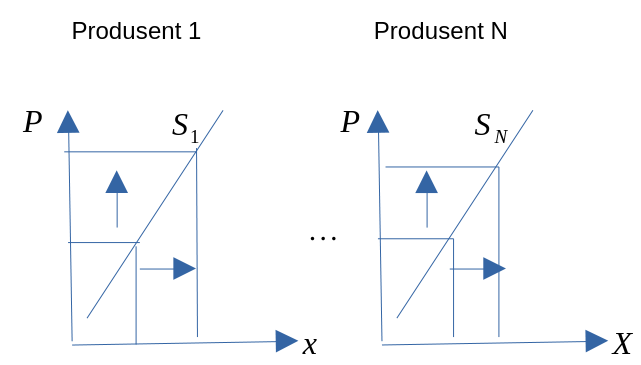
\includegraphics[width=0.65\textwidth,height=\textheight]{drawio/tkurve.png}

}

\caption{Figur 3.2}

\end{figure}%

\begin{center}\rule{0.5\linewidth}{0.5pt}\end{center}

\subsection{Markedslikevekt}\label{markedslikevekt}

\begin{itemize}
\tightlist
\item
  Utgangspunkt: markedets E-kurve og T-kurve.
\item
  Likevekt: dersom ingen aktører ønsker å endre den eksisterende
  økonomiske tilpasning.

  \begin{itemize}
  \tightlist
  \item
    \(X^S = X^D\)
  \end{itemize}
\end{itemize}

\begin{figure}[H]

{\centering 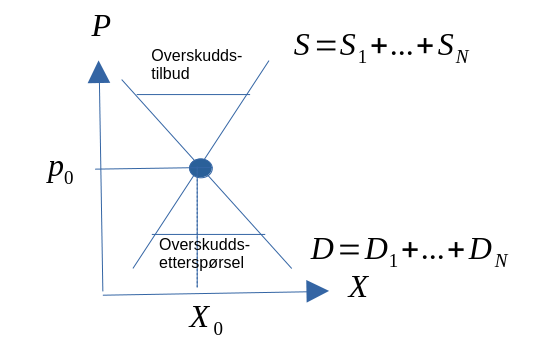
\includegraphics[width=0.5\textwidth,height=\textheight]{drawio/telikevekt.png}

}

\caption{Figur 3.3}

\end{figure}%

\begin{center}\rule{0.5\linewidth}{0.5pt}\end{center}

\begin{itemize}
\tightlist
\item
  Anta at prisen er lavere enn likevektspris (makspris).

  \begin{itemize}
  \tightlist
  \item
    Overskuddsetterspørsel: \(X^D > X^S\)
  \end{itemize}
\item
  Anta at prisen er over likevektsprisen (minpris).

  \begin{itemize}
  \tightlist
  \item
    Overskuddstilbud: \(X^S > X^D\)
  \end{itemize}
\item
  Merk: Ingenting i modellen som tilsier stabilitet. Men utenfor
  modellen kan vi resonnere markedskreftene alltid bringer oss tilbake
  til likevekt, slik det er beskrevet av Adam Smith.
\end{itemize}

\begin{center}\rule{0.5\linewidth}{0.5pt}\end{center}

\subsection{Konsument- produsent og sammfunnsøkonomisk
overskudd}\label{konsument--produsent-og-sammfunnsuxf8konomisk-overskudd}

\begin{itemize}
\tightlist
\item
  I samfunnsøkonomi er vi naturlig nok opptatt av å vurdere om et marked
  eller et prosjekt eller politikkforslag er samfunnsøkonomisk lønnsomt.
  Når alt kommer til alt er det jo høyest mulig velferd for individene i
  samfunnet som er målet.
\item
  For å vurdere velferden brukes begrepet samfunnsøkonomisk overskudd
  (SO).
\item
  Dette består av konsumentoverskudd (KO) og produsentoverskudd (PO)
\item
  Vi har derfor at SO er gitt ved: \begin{equation*}
  SO=PO+KO
  \end{equation*}
\end{itemize}

\begin{center}\rule{0.5\linewidth}{0.5pt}\end{center}

\subsubsection{Konsumentoverskudd}\label{konsumentoverskudd}

\begin{itemize}
\tightlist
\item
  Hvor mye du er villig til å betale for kalles Betalingsvillighet.
\item
  Betalingsvilligheten avhenger av hvor mye du har i utgangspunktet:
  \(\Rightarrow B(X)\)
\item
  Det et imidlertid forskjell på det konsumenten er villig til å betale,
  og det han faktisk betaler. Det er denne differensen som er
  konsumentoverskuddet:

  \begin{itemize}
  \tightlist
  \item
    \(\Rightarrow KO(X) = B(X) – PX\)
  \end{itemize}
\end{itemize}

\begin{figure}[H]

{\centering 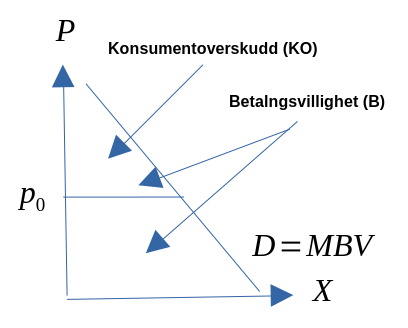
\includegraphics[width=0.5\textwidth,height=\textheight]{drawio/konso.png}

}

\caption{Figur 3.4}

\end{figure}%

\begin{center}\rule{0.5\linewidth}{0.5pt}\end{center}

\subsubsection{Produsentoverskudd}\label{produsentoverskudd}

\begin{itemize}
\tightlist
\item
  Produsentoverskudd defineres som summen av den ekstrainntekten som
  produsenten får, av å selge til en pris som er høyere enn den laveste
  de ville vært villige til å akseptere.
\item
  Det vil si: differensen mellom produsentens samlede salgsinntekter og
  variable kostnader.

  \begin{itemize}
  \tightlist
  \item
    \(\Rightarrow PO(X) = PX-CV(x)\)
  \end{itemize}
\end{itemize}

\begin{figure}[H]

{\centering 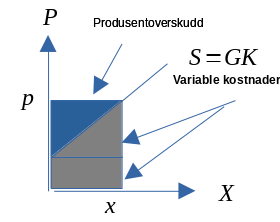
\includegraphics[width=0.4\textwidth,height=\textheight]{drawio/prodo.png}

}

\caption{Figur 3.5}

\end{figure}%

\begin{center}\rule{0.5\linewidth}{0.5pt}\end{center}

\subsubsection{Samfunnsøkonomisk overskudd og fullkommen
konkurranse}\label{samfunnsuxf8konomisk-overskudd-og-fullkommen-konkurranse}

\begin{itemize}
\item
  Maksimalt SO finner vi ved \begin{equation*}
  \underset{X}{\text{Maks}SO}=PO+KO=(PX-CV(X))+(B(X)-PX)
  \end{equation*}
\item
  Er løsningen til dette problemet tilfredsstilt i en markedsmodell med
  fullkommen konkurranse? JA (vi vil se nærmere på løsningen senere i
  dette kurset)!
\end{itemize}

\begin{center}\rule{0.5\linewidth}{0.5pt}\end{center}

\subsection{Komparativ statikk/ skift i
kurvene}\label{komparativ-statikk-skift-i-kurvene}

\begin{itemize}
\tightlist
\item
  Vi vet at tilbuds- og etterspørselskurvene er konstruert under en
  antagelse om at flere forhold antas konstante. Dersom det skjer
  endringer i noen av disse forholdene, vil kurvene forskyves i
  diagrammet. La oss se på noen av disse forholdene.
\end{itemize}

\textbf{Tilbudskurven}

\begin{itemize}
\tightlist
\item
  Ble tegnet for:

  \begin{itemize}
  \tightlist
  \item
    gitt teknologi for bedriften,
  \item
    gitte priser på innsatsfaktorene.
  \end{itemize}
\end{itemize}

\textbf{Etterspørselskurven}

\begin{itemize}
\tightlist
\item
  Ble tegnet for:

  \begin{itemize}
  \tightlist
  \item
    en gitt behovsstruktur for konsumenten,
  \item
    gitt samlet inntekt for konsumenten,
  \item
    gitt inntektsfordeling,
  \item
    gitte priser på andre goder.
  \end{itemize}
\end{itemize}

\begin{center}\rule{0.5\linewidth}{0.5pt}\end{center}

\textbf{Helningens betydning}

\begin{itemize}
\tightlist
\item
  Helningen på tilbuds- og etterspørselskurven påvirker hvordan
  endringer i markedet påvirker pris og mengde. La oss se på et eksempel
  der lavere pris på innsatsfaktorene har ført til et positivt skift i
  tilbudskurven.
\end{itemize}

Skiftanalyse (bratt/prisufølsom/prisuelastisk etterspørselskurve) :::
\{.cell\} ::: \{.cell-output-display\}
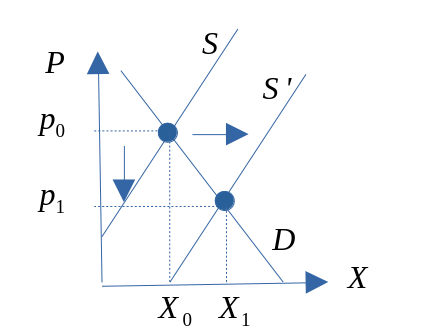
\includegraphics[width=0.5\textwidth,height=\textheight]{drawio/telikevekt_u.png}

:::

Skiftanalyse (slak/prisfølsom etterspørselskurve) ::: \{.cell\} :::
\{.cell-output-display\}
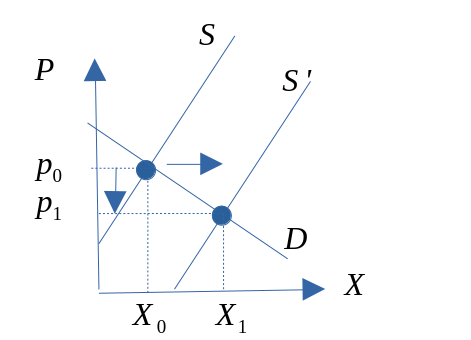
\includegraphics[width=0.5\textwidth,height=\textheight]{drawio/telikevekt_f.png}

::: :::

::::

\begin{center}\rule{0.5\linewidth}{0.5pt}\end{center}

\subsection{Effekten av en avgift}\label{effekten-av-en-avgift}

\begin{itemize}
\item
  En avgift kan ha flere hensikter, men spesielt er to ting viktig:

  \begin{enumerate}
  \def\labelenumi{\roman{enumi})}
  \tightlist
  \item
    Inntekt for staten
  \item
    Endrer markedsresultatet. Aktuelt ved behov for korrigering av
    nåværende situasjon (tilpasning).
  \end{enumerate}
\item
  Avgiften kan pålegges kjøperne og selgerne.
\item
  Anta nå at avgiften \(\tau\) blir pålagt selgerne
\end{itemize}

\begin{center}\rule{0.5\linewidth}{0.5pt}\end{center}

\begin{itemize}
\tightlist
\item
  Dersom avgiften pålegges produsentene, vil kostnadene til bedriften
  stige. Dette skifter isolert sett tilbudskurven innover. Den vertikale
  størrelsen på skiftet er lik avgiften \(\tau\). Resultater:
\item
  Staten får inn \(\tau\) kr. pr. enhet.
\item
  Konsumenten betaler: \(P^K\)
\item
  Produsenten mottar: \(P^P\) Produsenten ''sender'' nå avgiften til
  staten, men begge bærer byrden!!
\end{itemize}

\begin{figure}[H]

{\centering 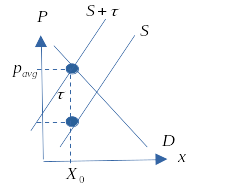
\includegraphics[width=0.45\textwidth,height=\textheight]{drawio/telikevekt_avg.png}

}

\caption{Figur 3.8}

\end{figure}%

\subsection{Maksimal- og minsteprisen}\label{maksimal--og-minsteprisen}

\textbf{Maksimalpris} har vi dersom markedsprisen blir overtyrt ved at
myndighetene setter et makspris som er \emph{lavere} enn markedsprisen.
::: \{.cell\} ::: \{.cell-output-display\}
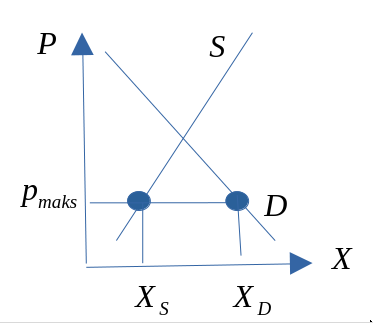
\includegraphics[width=0.5\textwidth,height=\textheight]{drawio/telikevekt_max.png}

:::

\textbf{Minstrepris} har vi dersom markedsprisen blir overtyrt ved at
myndighetene setter et minstepris som er \emph{høyere} enn
markedsprisen. ::: \{.cell\} ::: \{.cell-output-display\}
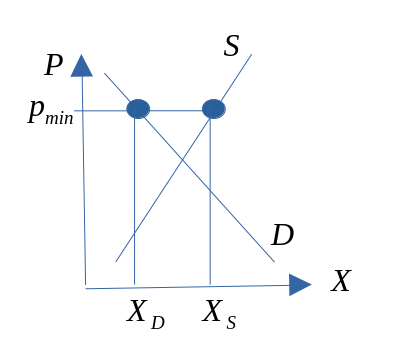
\includegraphics[width=0.5\textwidth,height=\textheight]{drawio/telikevekt_min.png}

::: :::

::::

\begin{center}\rule{0.5\linewidth}{0.5pt}\end{center}

\subsection{Produksjonsmulighetskurven
(PMK)}\label{produksjonsmulighetskurven-pmk}

\begin{itemize}
\tightlist
\item
  Produksjonsmulighetskurven (PMK)
\item
  PMK: kurven kan brukes til å illustrere hvordan produksjonsmulighetene
  er begrenset. Dette fører til et ressursallokeringsproblem. Videre
  skal vi illustrere forskjellen på kort og lang sikt.
\item
  Kurven bygger på en antagelse om at alternativkostnadene øker ved
  stadige overføringer av ressurser mellom sektorer.
\item
  Forutsetninger: to produkter, gitt mengde produksjonsfaktorer (kort
  sikt) og produksjonsteknologien er konstant.
\end{itemize}

\begin{figure}[H]

{\centering 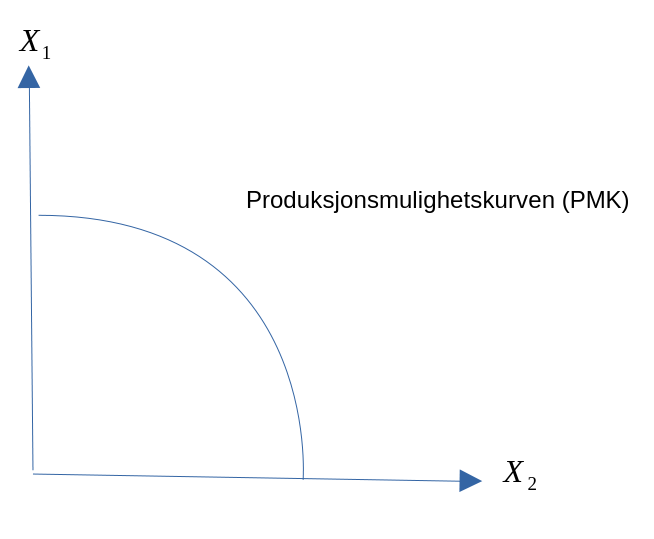
\includegraphics[width=1\textwidth,height=\textheight]{drawio/pmk.png}

}

\caption{Figur 3.11}

\end{figure}%

\section{Kapittel 4, 5 og 6: Innledning til
produsentteorien}\label{kapittel-4-5-og-6-innledning-til-produsentteorien}

\begin{center}\rule{0.5\linewidth}{0.5pt}\end{center}

\subsection{Produsentens rolle, teknologiske forhold og
produksjon}\label{produsentens-rolle-teknologiske-forhold-og-produksjon}

\begin{itemize}
\item
  Produsentene eller bedriftene er en av hovedaktørene i en økonomi.
\item
  Produsentens rolle: tilby de varer og tjenester som etterspørres i et
  samfunn. Basert på konsumentens ønsker må produsenten vite hva som
  skal produseres, mengde og lokalisering.
\item
  Teknologisk perspektiv: Produsenten bruker innsatsfaktorer til å
  omforme råvarer til ferdige produkter.
\item
  Vi forenkler produksjonsbildet ved å anta at produsenten bruker to
  innsatsfaktorer, \(N\) og \(K\), til å produsere ett produkt, \(x\).
  \(N\) er arbeidskraft og \(K\) er realkapital.
\end{itemize}

\begin{figure}[H]

{\centering 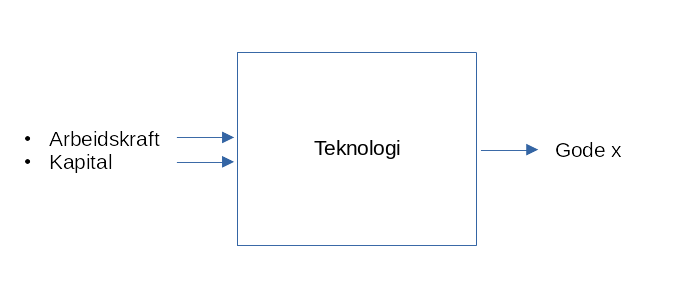
\includegraphics[width=1\textwidth,height=\textheight]{drawio/prodbildetf.png}

}

\caption{Figur 4.1}

\end{figure}%

\begin{center}\rule{0.5\linewidth}{0.5pt}\end{center}

\begin{itemize}
\item
  Bedriften må altså velge effektiv produksjonsprosess.
\item
  Økonomisk perspektiv: Her består valget i å velge hvor mye bedriften
  skal produsere og tilby av produktet.
\item
  For å kunne få størst mulig overskudd må vi kjenne til inntekter og
  kostnader. Kostnadene er igjen svært avhengig av det teknologiske
  valget.
\item
  Vi må derfor sammenkoble elementer fra begge disse perspektivene.
\item
  Vi tar utgangspunkt i produksjonsbildet med to innsatsfaktorer og ett
  produkt.

  \begin{itemize}
  \tightlist
  \item
    Produktfunksjonen:

    \begin{itemize}
    \tightlist
    \item
      \(x = f(N, K)\)
    \end{itemize}
  \item
    Viser, for enhver mulig faktorkombinasjon, det maksimale antall
    enheter som kan produseres av produktet.
  \item
    \(f\) beskriver formen på avhengighetsforholdet mellom
    produksjonsmengden og innsatsfaktorene. Kan tolkes som forhold
    (faktorer) som endrer produksjonsmengden uten å endre mengden av
    innsatsfaktorene \(N\) og \(K\).
  \end{itemize}
\end{itemize}

\begin{center}\rule{0.5\linewidth}{0.5pt}\end{center}

Merk: Til forskjell fra læreboka, vil vi forelesningene først gjennomgå
alle deler av produksjonsteorien på kort sikt, før vi ser på dette på
lang sikt.

\begin{longtable}[]{@{}lll@{}}
\toprule\noalign{}
Pensumbok & Kort sikt & Lang sikt \\
\midrule\noalign{}
\endhead
\bottomrule\noalign{}
\endlastfoot
Teknologi/Produksjon & Kap. 4 & Kap 4 \\
Inntekter og kostnader & Kap. 5 & Kap 5 \\
Optimering i produkt og faktormarkedene & Kap. 6 & Kap. 6 \\
\end{longtable}

\section{Kapittel 4, 5 og 6: Produksjonsteori på kort
sikt}\label{kapittel-4-5-og-6-produksjonsteori-puxe5-kort-sikt}

\begin{center}\rule{0.5\linewidth}{0.5pt}\end{center}

\subsection{Produksjon og teknologiske
forhold}\label{produksjon-og-teknologiske-forhold}

\emph{Talleksempel på en produktfunksjon} ::: \{.cell\} :::
\{.cell-output-display\}

\begin{table}
\centering
\begin{tabular}[t]{r|r|r|r|r}
\hline
Arbeidskraft (N) & Kapital (K) & Produksjon & Grenseprodukt. & Gjennomsnittsprod.\\
\hline
1 & 20 & 10 & NA & 10\\
\hline
2 & 20 & 24 & 14 & 12\\
\hline
3 & 20 & 39 & 15 & 13\\
\hline
\textbf{4} & \textbf{20} & \textbf{52} & \textbf{17} & \textbf{13}\\
\hline
\textbf{5} & \textbf{20} & \textbf{61} & \textbf{9} & \textbf{12}\\
\hline
\textbf{6} & \textbf{20} & \textbf{66} & \textbf{5} & \textbf{11}\\
\hline
7 & 20 & 66 & 0 & 9\\
\hline
8 & 20 & 64 & -2 & 8\\
\hline
9 & 20 & 56 & -8 & 6\\
\hline
10 & 20 & 44 & -12 & 4\\
\hline
\end{tabular}
\end{table}

::: :::

\begin{center}\rule{0.5\linewidth}{0.5pt}\end{center}

\textbf{Forutsetninger om produktfunksjonen}

\begin{itemize}
\tightlist
\item
  For analytiske formål antas funksjonen kontinuerlig og to ganger
  deriverbar:
\end{itemize}

Arbeidskraft

\begin{figure}[H]

{\centering 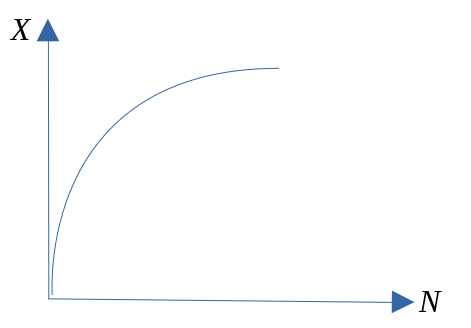
\includegraphics[width=0.8\textwidth,height=\textheight]{drawio/prodkl.png}

}

\caption{Figur 4KS.1}

\end{figure}%

\begin{itemize}
\tightlist
\item
  \(\frac{\partial f}{\partial N} > 0\)
\item
  \(\frac{\partial^2 f}{\partial N^2} < 0\)
\end{itemize}

\begin{itemize}
\tightlist
\item
  Positive, men avtagende grenseproduktiviteter.
\item
  De førsteordens partielle deriverte uttrykker grenseproduktiviteten:
  hvor mye produsert kvantum endres ved en liten endring i bruken av
  vedkommende innsatsfaktor.
\item
  Loven om avtakende utbytte gjelder altså her.
\end{itemize}

\begin{center}\rule{0.5\linewidth}{0.5pt}\end{center}

\subsection{Inntekter og kostnader}\label{inntekter-og-kostnader}

\subsubsection{Inntekter}\label{inntekter}

\begin{itemize}
\tightlist
\item
  Bedriftens inntekter bestemmes av antall enheter den selger, og prisen
  på disse enhetene.

  \begin{itemize}
  \tightlist
  \item
    Pris: \(p\). Mengde: \(x\).
  \item
    Inntekt: \(R=px\). Stigende i et \((x,R)\)-diagram
  \item
    Grenseinntekt: endring i inntekt ved en marginal endring i solgt
    kvantum: \(R'(x)\)
  \item
    Gjennomsnitsinntekt: inntekt per produsert enhet: \(\overline{R}\).
  \end{itemize}
\end{itemize}

\begin{center}\rule{0.5\linewidth}{0.5pt}\end{center}

\emph{Talleksempel for salgsinntekter}

\begin{tabular}[t]{r|l|l|l|l}
\hline
Solge enheter & Pris per enhet & Salgsinntekt & Grenseinntekt & Gjennomsnittsinntekt\\
\hline
1 & 1000 & 1000 &  & 1000\\
\hline
2 & 1000 & 2000 & 1000 & 1000\\
\hline
3 & 1000 & 3000 & 1000 & 1000\\
\hline
\end{tabular}

\begin{figure}[H]

{\centering 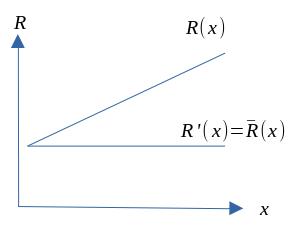
\includegraphics[width=0.5\textwidth,height=\textheight]{drawio/inntf.png}

}

\caption{Figur 5KS.1}

\end{figure}%

\begin{center}\rule{0.5\linewidth}{0.5pt}\end{center}

\subsubsection{Kostnader}\label{kostnader}

\begin{itemize}
\tightlist
\item
  Kostnader: De beløp som påløper som følge av virksomhet.

  \begin{itemize}
  \tightlist
  \item
    Faste kostnader \((C_F)\) : Kostnader som er uavhengige av produsert
    kvantum.
  \item
    Variable kostnader \((C_V\)): Varierer i takt med produsert kvantum
    - \(C_V = C_{V}(x)\)
  \item
    Totale kostnader \((C)\): Summen av faste og variable kostnader -
    \(C = C_F + C_V\)
  \item
    Gjennomsnittskostnader (enhetskostnader): Disse finner vi ved å
    dividere de respektive kostnadene med antall produserte enheter. -
    \(\overline{C}=\frac{C_F}{x}+\frac{C_V}{x}=\overline{C}_F+\overline{C}_V\)
  \item
    Grensekostnader ( \(GK\) eller \(C'\) ): Endringen i bedriftens
    totale kostnader ved en liten endring i produsert kvantum
  \end{itemize}
\end{itemize}

\begin{center}\rule{0.5\linewidth}{0.5pt}\end{center}

\textbf{Sammenhengen mellom gjennomsnittskostnad og grensekostnad}

\emph{Talleksempel a): med avtagende marginalproduktivitet (mest
relevant for dette kurset) og uten faste kostnader}

\begin{tabular}[t]{r|l|l|l}
\hline
Produserte enheter & Lønnskostnader & Antall arbeidere & Variable kostnader\\
\hline
1 & 1000 & 1 & 1000\\
\hline
2 & 1000 & 2 & 2000\\
\hline
3 & 1000 & 3.1 & 3100\\
\hline
\end{tabular}

::: \{.cell\} ::: \{.cell-output-display\}

\begin{tabular}[t]{l|l|l|l}
\hline
Faste kostnader & Totale kostnader & Grensekostnader & Gjennomsnittskostnad\\
\hline
0 & 1000 &  & \\
\hline
0 & 2000 & 1000 & 1000\\
\hline
0 & 3100 & 1100 & 1032\\
\hline
\end{tabular}

::: :::

\begin{center}\rule{0.5\linewidth}{0.5pt}\end{center}

\emph{Talleksempel b): med økende marginalproduktivitet (mindre
relevant) og uten faste kostnader}

\begin{tabular}[t]{r|l|l|l}
\hline
Produserte enheter & Lønnskostnader & Antall arbeidere & Variable kostnader\\
\hline
1 & 1000 & 1 & 1000\\
\hline
2 & 1000 & 2 & 2000\\
\hline
3 & 1000 & 2.9 & 2900\\
\hline
\end{tabular}

::: \{.cell\} ::: \{.cell-output-display\}

\begin{tabular}[t]{l|l|l|l}
\hline
Faste kostnader & Totale kostnader & Grensekostnader & Gjennomsnittskostnad\\
\hline
0 & 1000 &  & \\
\hline
0 & 2000 & 1000 & 1000\\
\hline
0 & 2900 & 900 & 966\\
\hline
\end{tabular}

::: :::

\begin{center}\rule{0.5\linewidth}{0.5pt}\end{center}

\emph{Talleksempel c): med avtagende marginalproduktivitet og med faste
kostnader}

\begin{tabular}[t]{r|l|l|l}
\hline
Produserte enheter & Lønnskostnader & Antall arbeidere & Variable kostnader\\
\hline
1 & 1000 & 1 & 1000\\
\hline
2 & 1000 & 2 & 2000\\
\hline
3 & 1000 & 3.1 & 3100\\
\hline
\end{tabular}

\begin{tabular}[t]{l|l|l|l}
\hline
Faste kostnader & Totale kostnader & Grensekostnader & Gjennomsnittskostnad\\
\hline
2000 & 3000 &  & 3000\\
\hline
2000 & 4000 & 1000 & 2000\\
\hline
2000 & 5100 & 1100 & 1700\\
\hline
\end{tabular}

\begin{center}\rule{0.5\linewidth}{0.5pt}\end{center}

\emph{Grensekostnad og gjennomsnittskostnad uten faste kostnader}

\begin{figure}[H]

{\centering 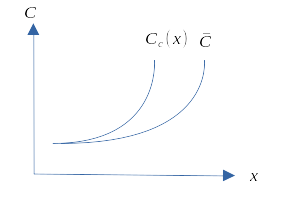
\includegraphics[width=0.5\textwidth,height=\textheight]{drawio/kostku.png}

}

\caption{Figur 5KS.3}

\end{figure}%

\emph{Grensekostnad og gjennomsnittskostnad med faste kostnader}

\begin{figure}[H]

{\centering 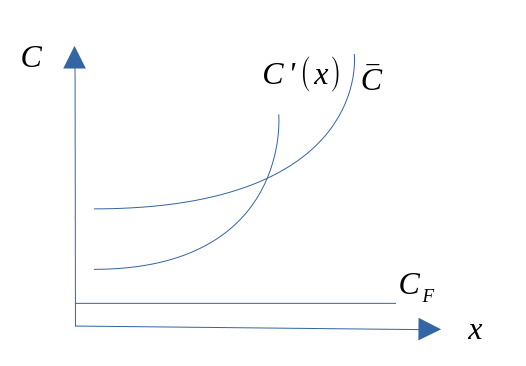
\includegraphics[width=0.5\textwidth,height=\textheight]{drawio/kostkm.png}

}

\caption{Figur 5KS.4}

\end{figure}%

\begin{center}\rule{0.5\linewidth}{0.5pt}\end{center}

\subsection{Tilpasningen i gode og
faktormarkedet}\label{tilpasningen-i-gode-og-faktormarkedet}

\begin{itemize}
\tightlist
\item
  Vi skal nå legge til grunn at bedriften har som mål å maksimere
  fortjenesten eller profitten.
\item
  Vi skal også legge til grunn av bedriften betrakter alle priser som
  gitte (gode- og faktorpriser).
\item
  Bedriften tilpasser seg på to markeder:

  \begin{itemize}
  \tightlist
  \item
    godemarkedet
  \item
    faktormarkedet: arbeidsmarkedet
  \end{itemize}
\item
  I faktormarkedet kjøper bedriften innsatsfaktorer og må velge de
  kvantum av faktorene som maksimerer fortjenesten.
\item
  I godemarkedet må bedriften velge den produksjonsmengden som
  maksimerer fortjenesten. Altså: to valg!
\end{itemize}

\begin{center}\rule{0.5\linewidth}{0.5pt}\end{center}

\subsubsection{Hvor stor skal produksjonen være og bedriftens tilbud av
produktet}\label{hvor-stor-skal-produksjonen-vuxe6re-og-bedriftens-tilbud-av-produktet}

\begin{itemize}
\tightlist
\item
  For å finne svar på dette, lar vi produksjonsmengden være variabel.
\item
  Hensikten med denne tilnærmingen er å analysere hvordan bedriften
  varierer produsert kvantum/ antall enheter den produserer, for å oppnå
  høyest mulig fortjeneste.
\item
  Produsentens valgvariabel er dermed kvantumet \(x\).
\item
  En fordel med denne tilnærmingen er at den gir sammenhengen mellom
  pris og produsert kvantum på en enkel måte. Dette kan så brukes til å
  utlede bedriftens tilbudskurve, og i neste omgang markedets
  tilbudskurve.
\end{itemize}

\begin{center}\rule{0.5\linewidth}{0.5pt}\end{center}

\textbf{Fortjenestemaksimering (kort sikt) med variabel
produksjonsmengde}

\begin{itemize}
\tightlist
\item
  Produksjon: \(x = f(N)\)
\item
  Kostnader: \(C(x) = C_V(x) + C_F\)
\item
  Salgsinntekt: \(R = px\)
\item
  Maks profitt: \(F = R – C\) som gir \(F=px – C_V(x) – C_F\)
\end{itemize}

Bedriften ønsker å maksimere dette uttrykket mhp. bruken av
arbeidskraften. Formelt kan vi uttrykke dette som: \[
\underset{x}{\text{Maks }} F=px-C(x)
\]

\begin{center}\rule{0.5\linewidth}{0.5pt}\end{center}

\textbf{Løsning og tolkning}

1.ordensbetingelsen er gitt ved \[
p = C'(x)
\] Produksjonen tilpasser seg der hvor produktprisen er lik
grensekostnaden.

2.ordensbetingelsen (som sikrer maksimum) \[
F''(x)=-C''(x) < 0 \Leftrightarrow C''(x) > 0 
\]

Kostnadsfunksjonen må være konveks (som vi tidligere har sett at kan
komme som et resultat av avtagende grenseproduktivitet mhp. bruken av
arbeidskraft)

\begin{center}\rule{0.5\linewidth}{0.5pt}\end{center}

\emph{Uten faste kostnader} ::: \{.cell\} ::: \{.cell-output-display\}
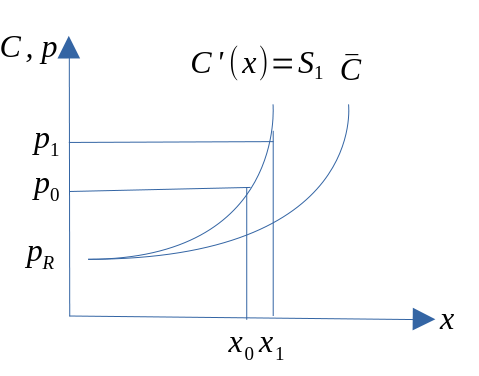
\includegraphics[width=0.45\textwidth,height=\textheight]{drawio/kgkufast.png}

:::

\emph{Med faste kostnader} ::: \{.cell\} ::: \{.cell-output-display\}
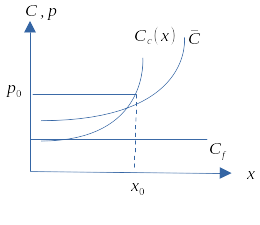
\includegraphics[width=0.45\textwidth,height=\textheight]{drawio/kgkmfast.png}

::: :::

::::

\begin{center}\rule{0.5\linewidth}{0.5pt}\end{center}

\begin{itemize}
\tightlist
\item
  Tilbudet til bedriften må bestemmes gjennom profittmaksimering eller
  kostnadsminimering.\\
\item
  Ettersom dette krever at bedriften er på grensekostnadskurven, vil
  tilbudskurven være ''den samme'' som grensekostnadskurven.
\item
  På kort vil bedriftens tilbud være stigende i et (x,p)-diagram.
\item
  Reservasjonsprisen (minsteprisen) vil være der hvor
  \(p_r=\overline{C}\)

  \begin{itemize}
  \tightlist
  \item
    Dersom de faste kostnadene er irrreversible (har en alternativ
    anvendelse), vil \(\overline{C}=\overline{C}_V\)
  \item
    Dersom de faste kostnadene er reversible (har en alternativ
    anvendelse), vil \(\overline{C}=\overline{C}_V+\overline{C}_F\)
  \end{itemize}
\end{itemize}

\begin{center}\rule{0.5\linewidth}{0.5pt}\end{center}

\textbf{Øvelse om produksjonen}

Anta at produktprisen er gitt ved 100 og kostnadsfunksjonen som
\(C(x)=x^2\). Hva blir den optimale produksjon?

\textbf{Løsning}

Uttrykket for fortjeneste kan formuleres som \[
F=100\cdot x - x^2
\]

Vi ønsker å finne maksimal produksjon. Førsteordensbetingelsen vil hær
være gitt ved \begin{equation*}
F'(x)=100-2x=0 \\
2x=100 \\
x=100/2=50
\end{equation*}

Andreordensbetingelsen for maksimum er oppfylt siden \[
F''(x)=-2<0
\]

Ved å sette \(x=50\) tilbake i uttrykket for profitt finner vi at
profitten er positiv og gitt ved \[
F=100\cdot 50 - 50^2=2500
\]

\begin{center}\rule{0.5\linewidth}{0.5pt}\end{center}

\subsubsection{Hvor stor skal etterspørselen etter arbeidskraft
være?}\label{hvor-stor-skal-etterspuxf8rselen-etter-arbeidskraft-vuxe6re}

\begin{itemize}
\tightlist
\item
  For å finne svar på dette spørsmålet betrakter vi innsatsfaktoren
  arbeidskraft som variable, og at disse utgjør beslutningsvariablene
  til bedriften.
\item
  Bedriften ønsker størst mulig overskudd.
\item
  Produksjon: \(x = f(N)\)
\item
  Kostnader: \(C = wN\)
\item
  Salgsinntekt: \(R = px\)
\item
  Profitten er gitt som inntekter (R) minus kostnader (C): \(F = R – C\)
\end{itemize}

Bedriften ønsker å maksimere dette uttrykket mhp. bruken av
arbeidskraften. Formelt kan vi uttrykke dette som: \[
\underset{N}{\text{Maks }} F=pf(N)-wN
\]

\begin{center}\rule{0.5\linewidth}{0.5pt}\end{center}

\textbf{Løsning og tolkning}

1.ordensbetingelsen er gitt ved \[
pf'(N)=W
\] Bruken av arbeidskraften bestemmes der hvor verdien av
grenseproduktiviteten er lik det nominelle lønnsnivået.

\begin{figure}[H]

{\centering 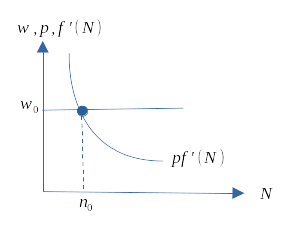
\includegraphics[width=0.5\textwidth,height=\textheight]{drawio/klearb.png}

}

\caption{Figur 6KS.4}

\end{figure}%

2.ordensbetingelsen (som sikrer optimum) \[
pf''(N) < 0
\]

\begin{center}\rule{0.5\linewidth}{0.5pt}\end{center}

\textbf{Øvelse om bruk av arbeidskraft}

Anta at produktprisen er gitt ved 10, lønnskostnadene gitt ved 1, og
produktfunsjonen \(x=\sqrt{N}\) Hva blir den optimale bruken av
arbeidskraft?

\textbf{Løsning}

Uttrykket for fortjeneste kan formuleres som \[
F=10N^{0.5}-N
\]

Vi ønsker å finne maksimal bruk av arbeidskraft. Førsteordensbetingelsen
vil være gitt ved

\begin{equation*}
F=1/2\cdot 10N^{0.5-1}-1=0 \\
5\cdot N^{(-0.5)}=1 \\
N^{-0.5}=1/5 \\
N^{0.5}=5 \\
N=5^2 = 25
\end{equation*}

2.ordensbetingelsen (som sikrer optimum) \(-2.5\cdot N^{-1.5} < 0\),
mens optimal forjeneste er positiv og gitt som
\(F=10\cdot 25^{1/2}-25=25\)

\section{Kapittel 4, 5 og 6: Produksjonsteori på lang
sikt}\label{kapittel-4-5-og-6-produksjonsteori-puxe5-lang-sikt}

\begin{center}\rule{0.5\linewidth}{0.5pt}\end{center}

\subsection{Produksjon og teknologiske
forhold}\label{produksjon-og-teknologiske-forhold-1}

\begin{itemize}
\tightlist
\item
  Vi tar utgangspunkt i produksjonsbildet med to innsatsfaktorer og ett
  produkt.
\item
  Produktfunksjonen:

  \begin{itemize}
  \tightlist
  \item
    \(x = f(N, K)\)
  \end{itemize}
\item
  Viser, for enhver mulig faktorkombinasjon, det maksimale antall
  enheter som kan produseres av produktet.
\item
  \(f\) beskriver formen på avhengighetsforholdet mellom
  produksjonsmengden og innsatsfaktorene. Kan tolkes som forhold
  (faktorer) som endrer produksjonsmengden uten å endre mengden av
  innsatsfaktorene \(N\) og \(K\).
\end{itemize}

\begin{center}\rule{0.5\linewidth}{0.5pt}\end{center}

Arbeidskraft ::: \{.cell\} ::: \{.cell-output-display\}
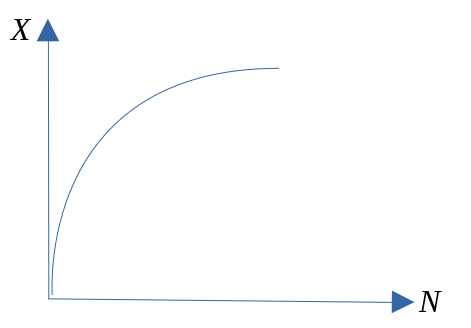
\includegraphics[width=1\textwidth,height=\textheight]{drawio/prodkl.png}

\begin{itemize}
\tightlist
\item
  \(\frac{\partial f}{\partial N} > 0\)
\item
  \(\frac{\partial^2 f}{\partial N^2} < 0\) :::
\end{itemize}

Kapital ::: \{.cell\} ::: \{.cell-output-display\}
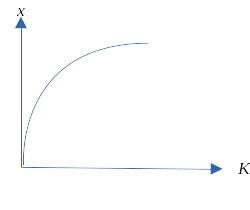
\includegraphics[width=1\textwidth,height=\textheight]{drawio/prodkk.png}

::: - \(\frac{\partial f}{\partial K} > 0\) -
\(\frac{\partial^2 f}{\partial K^2} < 0\) ::: ::::

\begin{center}\rule{0.5\linewidth}{0.5pt}\end{center}

\subsubsection{Isokvanter og MTSB for
produksjon}\label{isokvanter-og-mtsb-for-produksjon}

\begin{itemize}
\tightlist
\item
  For å representere produktfunksjonen grafisk, skal vi bruke et redskap
  fra matteboka, nemlig nivåkurver.
\item
  Nivåkurven kalles her en \emph{isokvant}: viser alle kombinasjoner av
  N og K som gir samme produserte kvantum.
\end{itemize}

\begin{figure}[H]

{\centering 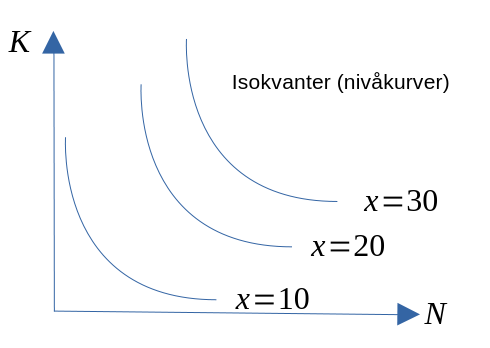
\includegraphics[width=1\textwidth,height=\textheight]{drawio/isokvant.png}

}

\caption{Figur 4LS.3}

\end{figure}%

\begin{center}\rule{0.5\linewidth}{0.5pt}\end{center}

\begin{itemize}
\tightlist
\item
  Isokvantens form bygger på følgende prinsipp: jo mer bedriften har av
  en innsatsfaktor, jo mer kan den bytte for én ekstra enhet av den
  andre faktoren, gitt at produksjonsmengden skal være den samme.
\item
  \emph{MTSB (marginale tekniske substiusjonsbrøk)} beskriver
  \emph{helningen} på en isokvant for en gitt faktorkombinasjon, dvs. i
  ett punkt på isokvanten.
\item
  Merk: MTSB er gitt ved forholdet mellom grenseproduktivitetene (se
  appendiks for formell utledning) \begin{equation*}
  MTSB \equiv -\frac{\Delta K}{\Delta N} =  \frac{f'_{N}(K,N)}{f'_{K}(K,N)}>0
  \end{equation*}
\item
  Formell utledning er vist i appendiks
\end{itemize}

\begin{center}\rule{0.5\linewidth}{0.5pt}\end{center}

\textbf{Eksempel 4.2 fra pensumbok}

Anta at produktfunksjonen er gitt ved: \(x = N^{0,7}+K^{0,3}\) Regn ut
MTSB for denne produktfunksjonen.

Grenseproduktiviteten til arbeidskraften er gitt ved \[
\frac{\partial x}{\partial N} = 0,7N^{0,7-1} =  0,7N^{-0,3} 
\]

Grenseproduktiviteten til kapitalen er gitt ved \[
\frac{\partial x}{\partial K} = 0,3K^{0,3-1} =  0,3K^{-0,7} 
\]

MTSB blir derfor \[
MTSB \equiv - \frac{\Delta K}{\Delta N} = \frac{\frac{\partial x}{\partial N}}{\frac{\partial x}{\partial K}} = \frac{0,7N^{-0,3}}{0,3K^{-0,7}} 
\]

\begin{center}\rule{0.5\linewidth}{0.5pt}\end{center}

\subsubsection{Substitusjonsegenskaper}\label{substitusjonsegenskaper}

\begin{itemize}
\tightlist
\item
  Dette sier noe om hvor lett det er å erstatte innsatsfaktorer med
  hverandre.
\item
  For eksempel: I noen bransjer er det lettere å erstatte arbeidskraft
  med kapital enn i andre.
\item
  Dette kan fremstilles med formen på isokvanten.
\item
  Ytterkantene: perfekt substitusjon og ingen substitusjon (perfekte
  komplementer).
\end{itemize}

Lineær produksjonsteknologi (perfekte substitutter) ::: \{.cell\} :::
\{.cell-output-display\}
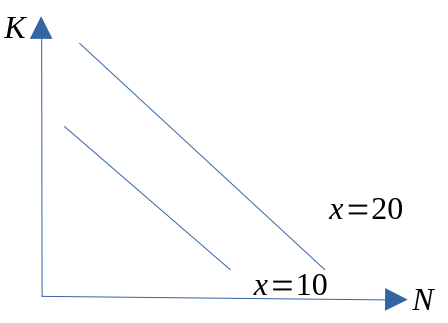
\includegraphics[width=0.7\textwidth,height=\textheight]{drawio/linsub.png}

:::

Leontief produksjonsteknologi (ingen substitusjon) ::: \{.cell\} :::
\{.cell-output-display\}
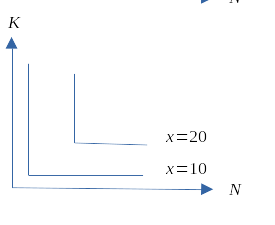
\includegraphics[width=0.7\textwidth,height=\textheight]{drawio/lensub.png}

::: :::

::::

\begin{center}\rule{0.5\linewidth}{0.5pt}\end{center}

\subsubsection{Skalaegenskaper}\label{skalaegenskaper}

\begin{itemize}
\tightlist
\item
  Mens grenseprodukt viser endring i bruken av én innsatsfaktor, viser
  skalaendringer endringer i bruken av \emph{alle} innsatsfaktorer.
\item
  Definisjon: Skalaegenskapene sier noe om hvor mye produksjonsmengden
  endres ved \emph{proporsjonale} endringer i bruken av
  innsatsfaktorene.
\item
  Proporsjonale endringer innebærer at forholdet mellom N og K er
  konstant.
\item
  Anta en proporsjonal økning på 100\%.

  \begin{itemize}
  \tightlist
  \item
    Hva skjer med produksjonsmengden (merk: produksjonsprosesser kan
    variere i skala)?
  \end{itemize}
\end{itemize}

\begin{center}\rule{0.5\linewidth}{0.5pt}\end{center}

\begin{itemize}
\item
  \begin{enumerate}
  \def\labelenumi{\roman{enumi})}
  \tightlist
  \item
    Konstant skalautbytte
  \end{enumerate}

  \begin{itemize}
  \tightlist
  \item
    Skalaøkning på y \% \(\Rightarrow\) økning i produsert kvantum på y
    \%.
  \end{itemize}
\end{itemize}

\begin{figure}[H]

{\centering 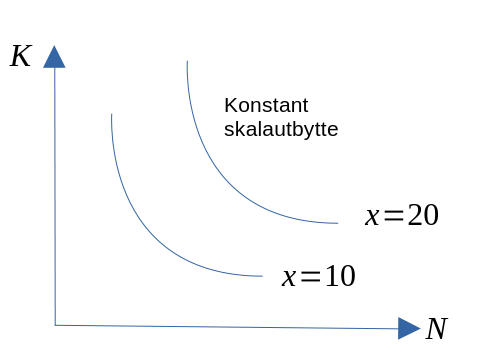
\includegraphics[width=0.4\textwidth,height=\textheight]{drawio/koskala.png}

}

\caption{Figur 4LS.6}

\end{figure}%

\begin{itemize}
\item
  \begin{enumerate}
  \def\labelenumi{\roman{enumi})}
  \setcounter{enumi}{1}
  \tightlist
  \item
    Avtagende skalautbytte
  \end{enumerate}

  \begin{itemize}
  \tightlist
  \item
    Skalaøkning på y \% \(\Rightarrow\) økning i produsert kvantum på
    mindre enn y \%.
  \end{itemize}
\end{itemize}

\begin{figure}[H]

{\centering 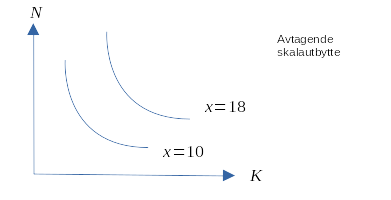
\includegraphics[width=0.4\textwidth,height=\textheight]{drawio/avskala.png}

}

\caption{Figur 4LS.7}

\end{figure}%

\begin{itemize}
\item
  \begin{enumerate}
  \def\labelenumi{\roman{enumi})}
  \setcounter{enumi}{2}
  \tightlist
  \item
    Økende skalautbytte
  \end{enumerate}

  \begin{itemize}
  \tightlist
  \item
    Skalaøkning på y \% \(\Rightarrow\) økning i produsert kvantum på
    mer enn y \%.
  \end{itemize}
\end{itemize}

\begin{figure}[H]

{\centering 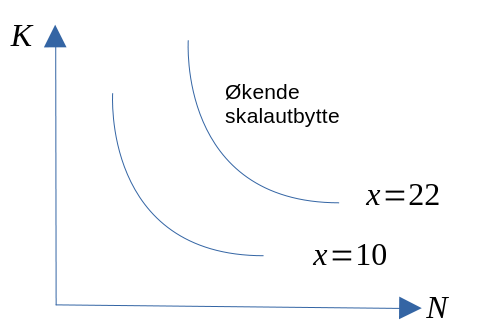
\includegraphics[width=0.4\textwidth,height=\textheight]{drawio/okskala.png}

}

\caption{Figur 4LS.8}

\end{figure}%

\begin{center}\rule{0.5\linewidth}{0.5pt}\end{center}

\subsection{Inntekter og kostnader}\label{inntekter-og-kostnader-1}

\subsubsection{Inntekter}\label{inntekter-1}

\begin{itemize}
\tightlist
\item
  Sammenlignet med den beskrivelsen som ble gitt for kort sikt,
  forekommer det her ingen endringer.
\end{itemize}

\begin{center}\rule{0.5\linewidth}{0.5pt}\end{center}

\subsubsection{Kostnader}\label{kostnader-1}

\begin{itemize}
\tightlist
\item
  Sammenlignet med den beskrivelsen som ble gitt for kort sikt, kan vi
  her se bort fra de faste kostnadene siden vi antar alle
  innsatsfaktorer for å være variable på lang sikt.
\end{itemize}

\subsubsection{Kostnadslinjen og
isokostlinja}\label{kostnadslinjen-og-isokostlinja}

\begin{itemize}
\tightlist
\item
  Totale kostnader for bedriften er summen av variable og faste
  kostnader. La oss nå se bort fra de faste, dette siden vi antar alle
  faktorer antas å være variable på lang sikt.
\item
  Vi antar at bedriftens kostnader kan uttrykkes ved summen av utgiftene
  på de to innsatsfaktorene.

  \begin{itemize}
  \tightlist
  \item
    Pris på N: w
  \item
    Pris på K: r
  \end{itemize}
\item
  \(C = wN + rK\) Totale kostnader (C) er da gitt ved: \[
  C = wN  +  rK
  \]
\end{itemize}

\begin{center}\rule{0.5\linewidth}{0.5pt}\end{center}

\begin{itemize}
\tightlist
\item
  Isokost (låser totalkostnadene til et bestemt nivå) \(C^o=C\) \[
  C^o= wN + rK
  \]

  \begin{itemize}
  \tightlist
  \item
    Helningen på isokostlinja \begin{equation}
    \Delta C^0= w\Delta N + r\Delta K = 0 \\
     r\Delta K = -w\Delta N  \\
    \frac{\Delta K}{\Delta N} = - \frac{w}{r} 
    \end{equation}
  \end{itemize}
\end{itemize}

\begin{center}\rule{0.5\linewidth}{0.5pt}\end{center}

\begin{itemize}
\tightlist
\item
  Bruker hele budsjettet på arbeidskraft \(\Rightarrow K=0\)
  \begin{equation}
  C^0= wN + r0 = wN \\
  C^0/w = N \\
  N = C^0/w 
  \end{equation}
\item
  Bruke hele budsjettet (kostnaden) på kapital \(\Rightarrow N=0\)
  \begin{equation}
  C^0= w0 + rK = wN \\
  C^0/r = K \\
  K = C^0/r 
  \end{equation}
\end{itemize}

\begin{center}\rule{0.5\linewidth}{0.5pt}\end{center}

\subsubsection{Maksimering av produksjonen for en gitt kostnadsramme
(optimal
tilpasning)}\label{maksimering-av-produksjonen-for-en-gitt-kostnadsramme-optimal-tilpasning}

\begin{itemize}
\tightlist
\item
  Målsetting er her å maksimere produsert kvantum innenfor en gitt
  kostnadsramme.
\item
  Dette kan være typisk for en bedrift i offentlig sektor, der de
  økonomiske rammebetingelsene utgjøres av en gitt kostnadsramme eller
  et gitt budsjett som er blitt tildelt over de offentlige budsjetter.
\end{itemize}

\begin{center}\rule{0.5\linewidth}{0.5pt}\end{center}

\begin{itemize}
\tightlist
\item
  Tar utgangspunkt i produktfunksjonen:

  \begin{itemize}
  \tightlist
  \item
    \(x = f(N, K)\)
  \end{itemize}
\item
  Helningen er gitt ved MTSB.
\item
  Tar så utgangspunkt i kostnadslinja:

  \begin{itemize}
  \tightlist
  \item
    \(C = wN + rK\)
  \end{itemize}
\item
  Kombinerer disse for å finne optimal tilpasning.
\end{itemize}

Max \(x=f(K,N)\) gitt \(C^0=wN +rK\) gitt (beskrankning)

\begin{center}\rule{0.5\linewidth}{0.5pt}\end{center}

Dette problemet kan løses ved bruk av Lagrange-metode (se appendiks for
formell utledning), hvor løsningen er gitt ved:

\begin{equation}
MTSB \equiv  \frac{f'_{N}}{f'_{K}} = \frac{w}{r} \\
C^0=wN +rK
\end{equation}

Optimal løsning er her karakterisert ved tangeringspunktet mellom
isokvant og isokostlinjen.

\begin{figure}[H]

{\centering 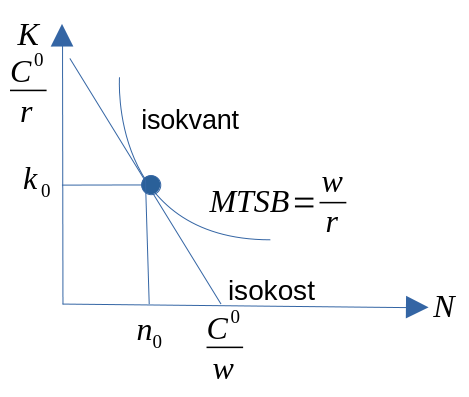
\includegraphics[width=1\textwidth,height=\textheight]{drawio/kosmin.png}

}

\caption{Figur 5LS.1}

\end{figure}%

\begin{center}\rule{0.5\linewidth}{0.5pt}\end{center}

\paragraph{Substitumalen: økonomisk
substitusjon}\label{substitumalen-uxf8konomisk-substitusjon}

\begin{itemize}
\item
  Dersom vi tenker oss flere endringer i bedriftens kostnadsramme med
  tilhørende optimale isokvant, vil vi få frem en rekke
  tangeringspunkter. ::: \{.cell\} ::: \{.cell-output-display\}
  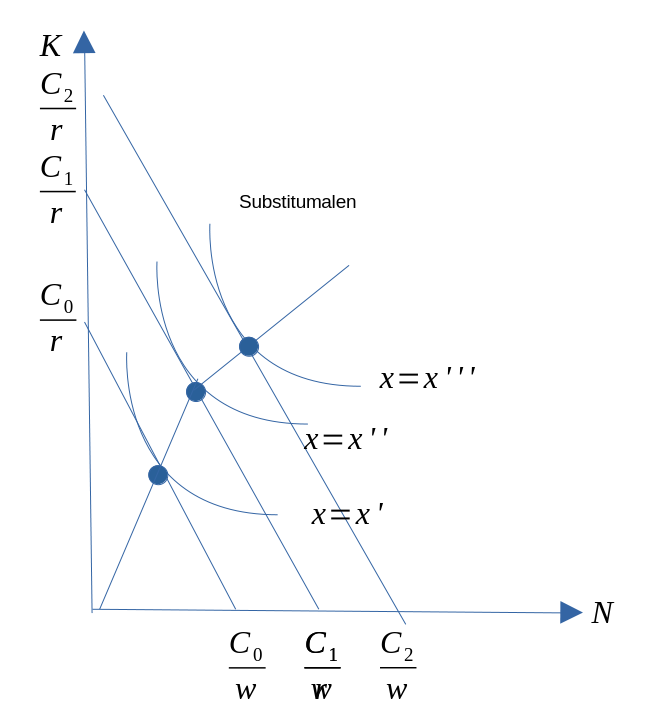
\includegraphics[width=1\textwidth,height=\textheight]{drawio/submalen.png}
  ::: :::
\item
  Kurven gjennom alle disse punktene kalles \emph{ekspansjonsveien}
  eller \emph{substitumalen}.
\item
  På ethvert punkt på denne kurven kan det leses av produksjonsmengde,
  tilhørende kostnader og etterspørsel etter innsatsfaktorer.
\item
  Alle punktene på substitumalen viser tilpasninger der det ikke er
  mulig å øke produktmengden, uten at kostnadene øker. Det er heller
  ikke mulig å redusere kostnadene, uten samtidig å redusere produsert
  kvantum.
\item
  Dersom bedriften er utenfor substitumalen kan den alltid bedre sin
  situasjon ved økonomisk substitusjon.
\end{itemize}

\begin{center}\rule{0.5\linewidth}{0.5pt}\end{center}

\subsection{Tilpasningen i gode og
faktormarkedet}\label{tilpasningen-i-gode-og-faktormarkedet-1}

\subsubsection{Hvor stor skal produksjonen være og bedriftens tilbud av
produktet}\label{hvor-stor-skal-produksjonen-vuxe6re-og-bedriftens-tilbud-av-produktet-1}

\begin{itemize}
\tightlist
\item
  Tilbudet til bedriften må bestemmes gjennom profittmaksimering eller
  kostnadsminimering.\\
\item
  Ettersom dette krever at bedriften er på grensekostnadskurven, vil
  tilbudskurven være ''den samme'' som grensekostnadskurven.
\end{itemize}

\begin{center}\rule{0.5\linewidth}{0.5pt}\end{center}

\begin{itemize}
\tightlist
\item
  På lang sikt vil bedriftens tilbudskurve enten være

  \begin{itemize}
  \tightlist
  \item
    Stigende (ved avtagende skalautbytte) i et (x,p)-diagram
  \item
    Horisontal (ved konstant skalautbytte) i et (x,p)-diagram
  \item
    Avtagende (ved økende skalautbytte) i et (x,p)-diagram
  \end{itemize}
\end{itemize}

\begin{figure}[H]

{\centering 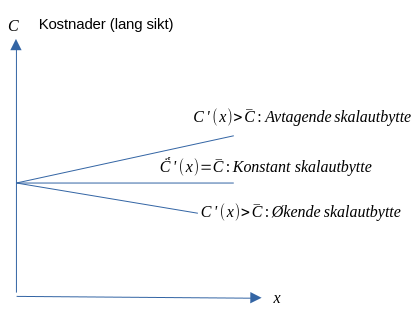
\includegraphics[width=1\textwidth,height=\textheight]{drawio/til_lang.png}

}

\caption{Figur 5LS.3}

\end{figure}%

\begin{center}\rule{0.5\linewidth}{0.5pt}\end{center}

\subsubsection{Hvor stor skal etterspørselen etter arbeidskraft og
kapital
være?}\label{hvor-stor-skal-etterspuxf8rselen-etter-arbeidskraft-og-kapital-vuxe6re}

\textbf{Redusert pris på kapital}

\begin{figure}[H]

{\centering 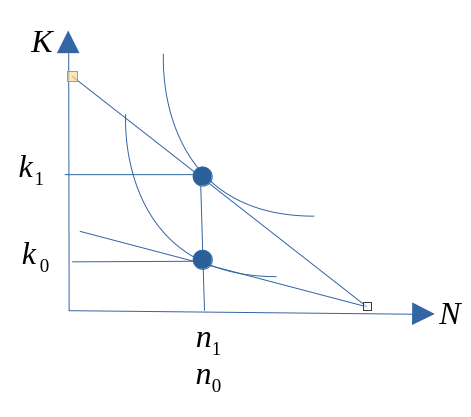
\includegraphics[width=0.3\textwidth,height=\textheight]{drawio/kosminkk.png}

}

\caption{Figur 6LS.1}

\end{figure}%

\begin{center}\rule{0.5\linewidth}{0.5pt}\end{center}

\textbf{Redusert pris på arbeidskraft}

\begin{figure}[H]

{\centering 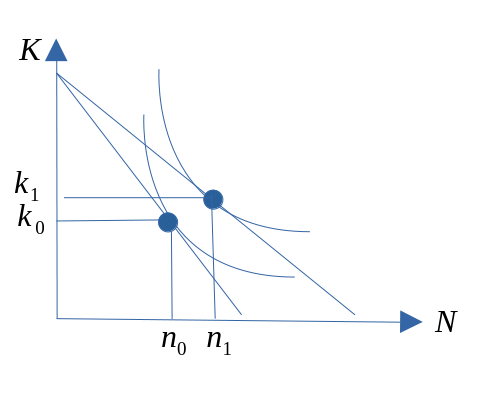
\includegraphics[width=0.3\textwidth,height=\textheight]{drawio/kosminka.png}

}

\caption{Figur 6LS.2}

\end{figure}%

Generelt resultat: Etterspør mer (mindre) av den innsatsfaktoren som har
blitt billigere (dyrere), og den kvantative effekten her er sterkere på
langt sikt enn på kort sikt pga. substitusjonsegenskapene mellom
arbeidskraft og kapital.

\subsection{Appendiks}\label{appendiks}

\subsubsection{MTSB: Formell utledning}\label{mtsb-formell-utledning}

Formell utledning av MTSB. Ta utgangspunkt i produktfunksjonen og total
differensier.

\[
\overline{x} = f(K,N)
\]

Dersom vi totaldifferensierer dette uttrykket får vi

\begin{equation*}
\Delta \overline{x} = f'_{K}(K,N)\Delta K + f'_{N}(K,N)\Delta N = 0 
\end{equation*}

Uttrykket ovenfor kan skrives som

\begin{equation*}
f'_{K}(K,N)\Delta K =- f'_{N}(K,N)\Delta N \\
\frac{\Delta K}{\Delta N} = - \frac{f'_{N}(K,N)}{f'_{K}(K,N)} 
\end{equation*}

\begin{equation*}
MTSB \equiv -\frac{\Delta K}{\Delta N} =  \frac{f'_{N}(K,N)}{f'_{K}(K,N)}>0
\end{equation*}

Merk: MTSB er gitt ved forholdet mellom grenseproduktivitetene.

\begin{center}\rule{0.5\linewidth}{0.5pt}\end{center}

\subsubsection{Lagrange: Produktmaksimering for en gitt
kostnadsramme}\label{lagrange-produktmaksimering-for-en-gitt-kostnadsramme}

Maks \(x=f(K,N)\) gitt \(C^0=wN +rK\) gitt (beskrankning). Lagrange
metode: \begin{equation}
L = f(K,N) - \lambda(wN+rK-C^0)
\end{equation} Første ordens betingelsen er gitt ved \begin{equation}
\partial L/\partial N = f'_{N} - \lambda w  =0 \\ 
\partial L/\partial K = f'_{K} - \lambda r =0 \\
C^0=wN +rK
\end{equation}

\begin{center}\rule{0.5\linewidth}{0.5pt}\end{center}

Kombinerer de to første ordens betingelsene gir oss to likninger for å
løse de to ukjente N,K \begin{equation}
MTSB \equiv  \frac{f'_{N}}{f'_{K}} = \frac{w}{r} \\
C^0=wN +rK
\end{equation} Optimal løsning er her karakterisert ved
tangeringspunktet mellom isokvant og isokostlinjen.

Ved å sette inn for den optimale løsningen av \(N\) og \(K\) finner vi
det optimale produksnivået (sammensetningen av N og K som gjør
produksjen størst mulig).

\begin{center}\rule{0.5\linewidth}{0.5pt}\end{center}

\subsubsection{Lagrange: Kostnadsminimering for en gitt
produksjon}\label{lagrange-kostnadsminimering-for-en-gitt-produksjon}

Min \(C=wN +rK\) gitt \(x^0=f(K,N)\) gitt (beskrankning). Lagrange
metode: \begin{equation}
L =wN +rK - \lambda(f(K,N)-x^0)
\end{equation} Første ordens betingelsen er gitt ved \begin{equation}
\partial L/\partial N = f'_{N} - \lambda w  =0 \\ 
\partial L/\partial K = f'_{K} - \lambda r =0 \\
x^0=f(K,N)
\end{equation}

\begin{center}\rule{0.5\linewidth}{0.5pt}\end{center}

Kombinerer de to første ordens betingelsene gir oss to likninger for å
løse de to ukjente N,K \begin{equation}
MTSB \equiv  \frac{f'_{N}}{f'_{K}} = \frac{w}{r} \\
x^0=f(K,N)
\end{equation} Optimal løsning også her karakterisert ved
tangeringspunktet mellom isokvant og isokostlinjen.

\textbf{Merk}:

\begin{itemize}
\tightlist
\item
  Ved å sette inn for den optimale løsningen av \(N\) og \(K\) finner vi
  bedriftens kostnadsfunksjon (kostnaden som minimerer produksjonen for
  et gitt produksjonsnivå).
\item
  Grensekostnaden vil derfor framkomme ved å derivere den funksjonen mhp
  produsert kvantum (see figur 5LS.3).
\end{itemize}

\section{Kapittel 7: Konsumentteori}\label{kapittel-7-konsumentteori}

\begin{center}\rule{0.5\linewidth}{0.5pt}\end{center}

\subsection{Innledning}\label{innledning-1}

\begin{itemize}
\tightlist
\item
  Vi skal i det følgende forsøke å illustrere hvordan en
  konsument/husholdning tilpasser seg i et godemarked.
\item
  Husholdning: gruppe av individer med samme preferanser.
\item
  Selvbergingsøkonomi \(\Rightarrow\) bytteøkonomi \(\Rightarrow\)
  pengeøkonomi
\item
  Vi skal anta at konsumenten tilpasser seg slik at nytten ved å
  forbruke de ulike godene blir størst mulig.
\item
  \textbf{Men:} konsumenten står ovenfor noen restriksjoner
  (betingelser).
\end{itemize}

\begin{center}\rule{0.5\linewidth}{0.5pt}\end{center}

\subsection{Nytteteori}\label{nytteteori}

\begin{itemize}
\tightlist
\item
  Vi kan dele nytteteori i to:

  \begin{enumerate}
  \def\labelenumi{\arabic{enumi}.}
  \tightlist
  \item
    Kardinal nytte:

    \begin{itemize}
    \tightlist
    \item
      Nytten kan måles.
    \end{itemize}
  \item
    Ordinal nytte:

    \begin{itemize}
    \tightlist
    \item
      Ikke målbar nytte. Her forutsetter vi at konsumenten kan ordne
      eller rangere de ulike godekombinasjonene.
    \end{itemize}
  \end{enumerate}
\end{itemize}

\begin{center}\rule{0.5\linewidth}{0.5pt}\end{center}

\subsection{Hvilke sentrale faktorer bestemmer etterspørselen etter et
gode?}\label{hvilke-sentrale-faktorer-bestemmer-etterspuxf8rselen-etter-et-gode}

Vi tar utgangspunkt i følgende spørsmål: Hvilke forhold vil være av
\emph{størst} betydning for en konsuments etterspørsel etter et gode?

\begin{itemize}
\tightlist
\item
  Sentrale faktorer:
\item
  Konsumentens behovstruktur
\item
  Konsumentens inntekt
\item
  Prisen på godet
\item
  Prisen på andre goder
\end{itemize}

\begin{center}\rule{0.5\linewidth}{0.5pt}\end{center}

\subsection{Forenklet fremstilling av konsumentens preferanser og
behovsstruktur}\label{forenklet-fremstilling-av-konsumentens-preferanser-og-behovsstruktur}

\begin{itemize}
\tightlist
\item
  Vi forenkler ved å anta at konsumenten kan velge mellom kun to goder:
  \(x_1\) og \(x_2\).
\item
  Ved å konsumere de to godene oppnår konsumenten en nytte: U.
\item
  For å kunne behandle dette formelt, blir vi nødt å gjøre noen
  antagelser om konsumentens preferanser:

  \begin{enumerate}
  \def\labelenumi{\arabic{enumi}.}
  \tightlist
  \item
    Determinerthetsaksiomet
  \item
    Ikkemetningsaksiomet
  \item
    Transitivitetsaksiomet
  \end{enumerate}
\end{itemize}

\begin{center}\rule{0.5\linewidth}{0.5pt}\end{center}

\begin{itemize}
\tightlist
\item
  Når disse forutsetningene (aksiomene) er oppfylt, vil det i prinsippet
  være mulig å uttrykke hvilken nytte konsumenten får av å konsumere de
  to godene med en nyttefunksjon:

  \begin{itemize}
  \tightlist
  \item
    \(U = u(x_1, x_2)\)
  \end{itemize}
\item
  En nyttefunksjon viser for enhver godekombinasjon den samlede nytte
  konsumenten oppnår ved å konsumere denne godekombinasjonen.
\item
  For analytiske formål antas denne funksjonen å være kontinuerlig og to
  ganger deriverbar.
\end{itemize}

\begin{center}\rule{0.5\linewidth}{0.5pt}\end{center}

\subsubsection{Grensenytte}\label{grensenytte}

\begin{itemize}
\tightlist
\item
  Grensenytten av et gode uttrykker den endring konsumenten får i sin
  nytte ved en liten endring i tilgangen på det godet.
\item
  Vi skal anta at tilleggsnytten er positiv:

  \begin{itemize}
  \tightlist
  \item
    \(u'_{x_{1}}(x_1,x_2)>0\) og \(u'_{x_{2}}(x_1,x_2)>0\)
  \end{itemize}
\item
  Videre er det også vanlig å anta at nytteøkningen i tillegg er
  avtagende:

  \begin{itemize}
  \tightlist
  \item
    \(u''_{x_{1}}(x_1,x_2)<0\) og \(u''_{x_{2}}(x_1,x_2)<0\)
  \end{itemize}
\item
  \textbf{Altså}: - Konsumenten har positive, men avtagende
  grensenytter.
\end{itemize}

\begin{figure}[H]

{\centering 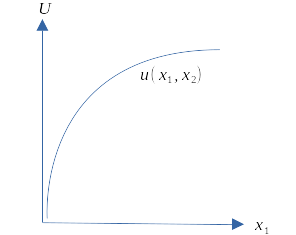
\includegraphics[width=1\textwidth,height=\textheight]{drawio/grensenytte.png}

}

\caption{Figur 7.1}

\end{figure}%

\begin{center}\rule{0.5\linewidth}{0.5pt}\end{center}

\subsubsection{Indifferenskurve}\label{indifferenskurve}

\begin{itemize}
\tightlist
\item
  Nyttefunksjonen kan representeres grafisk med indifferenskurver.
\item
  OBS: Merk at nyttefunksjonen har tre ukjente. Vi må derfor operere med
  et tre-dimensjonalt diagram. Dette vil vi unngå. Ved å sette de
  uavhengige variablene (\(x_{1},x_{2}\)) på aksene i et to-dimensjonalt
  diagram, kan funksjonen illustreres grafisk for gitte verdier på den
  tredje variabelen, U.
\end{itemize}

\begin{figure}[H]

{\centering 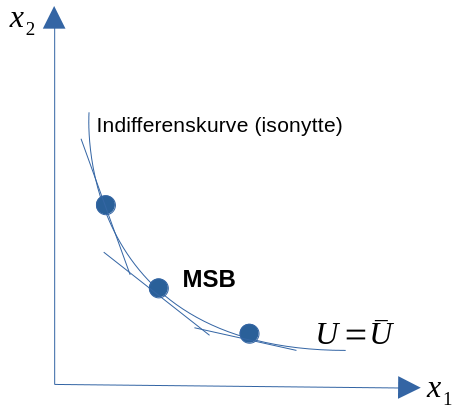
\includegraphics[width=1\textwidth,height=\textheight]{drawio/indkurve.png}

}

\caption{Figur 7.2}

\end{figure}%

\begin{itemize}
\tightlist
\item
  Indifferenskurven viser altså alle kombinasjoner av de to godene som
  gir konsumenten samme totale nytte.
\end{itemize}

\begin{center}\rule{0.5\linewidth}{0.5pt}\end{center}

\subsubsection{Forklaring på indifferenskurvens form og marginal
substitusjonsbrøk
(MSB)}\label{forklaring-puxe5-indifferenskurvens-form-og-marginal-substitusjonsbruxf8k-msb}

\begin{itemize}
\tightlist
\item
  Kurven heller nedover pga. ikkemetningsaksiomet. Videre ser vi at
  kurven er konveks mot origo.
\item
  Det skyldes følgende antagelse: Desto mer du har av \(x_1\), jo mindre
  vil du gi opp av \(x_2\) for å få mer av \(x_1\).

  \begin{itemize}
  \tightlist
  \item
    Loven om fallende MSB.
  \end{itemize}
\item
  MTSB er gitt som (se appendiks for matematisk utledning)
  \begin{equation*}
  MSB\equiv - \frac{\Delta x_{2}}{\Delta x_{1}}  = \frac{u'_{x_{1}}}{u'_{x_{2}}}
  \end{equation*}
\end{itemize}

\begin{center}\rule{0.5\linewidth}{0.5pt}\end{center}

\subsubsection{Indifferenskart}\label{indifferenskart}

\begin{itemize}
\tightlist
\item
  MSB viser altså antall enheter som en konsument er villig til å gi
  opp, for å få én ekstra enhet av det andre godet.

  \begin{itemize}
  \tightlist
  \item
    Bytteforholdet mellom to goder, gitt et konstant nyttenivå.
  \item
    For å få frem ulike nyttenivåer må vi således tegne et
    indifferenskart.
  \end{itemize}
\end{itemize}

\begin{figure}[H]

{\centering 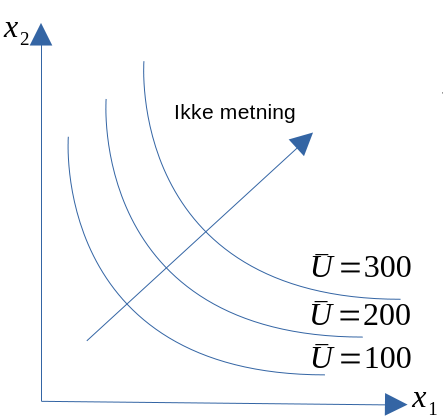
\includegraphics[width=0.35\textwidth,height=\textheight]{drawio/indkart.png}

}

\caption{Figur 7.3}

\end{figure}%

\begin{center}\rule{0.5\linewidth}{0.5pt}\end{center}

\subsubsection{Andre former på
indifferenskurven}\label{andre-former-puxe5-indifferenskurven}

Ingen substitusjonsmuligheter

\begin{figure}[H]

{\centering 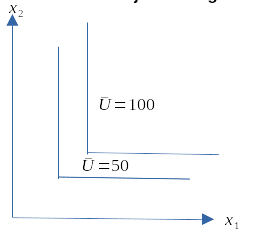
\includegraphics[width=0.5\textwidth,height=\textheight]{drawio/subsingen.png}

}

\caption{Figur 7.4}

\end{figure}%

Perfekte substitusjonsmuligheter

\begin{figure}[H]

{\centering 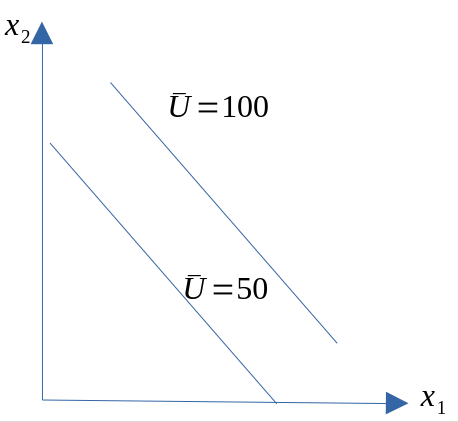
\includegraphics[width=0.5\textwidth,height=\textheight]{drawio/subsperf.png}

}

\caption{Figur 7.5}

\end{figure}%

\begin{center}\rule{0.5\linewidth}{0.5pt}\end{center}

\textbf{Øvelse om MSB}

\begin{enumerate}
\def\labelenumi{\arabic{enumi}.}
\tightlist
\item
  Anta at \(u(x_1,x_2) = 10x_1x_2\). Finn uttrykket for MSB.
\end{enumerate}

\textbf{Svar} \begin{equation*}
MSB = \frac{10x_2}{10x_1}= \frac{x_2}{x_1}
\end{equation*}

\begin{center}\rule{0.5\linewidth}{0.5pt}\end{center}

\begin{enumerate}
\def\labelenumi{\arabic{enumi}.}
\setcounter{enumi}{1}
\tightlist
\item
  Beregn nyttenivået, vis og illustrer inndifferenskurven for de tre
  verdiene nedenfor:
\end{enumerate}

\begin{itemize}
\tightlist
\item
  \begin{enumerate}
  \def\labelenumi{(\roman{enumi})}
  \tightlist
  \item
    \(x_1=2,x_2=4\)
  \end{enumerate}
\item
  \begin{enumerate}
  \def\labelenumi{(\roman{enumi})}
  \setcounter{enumi}{1}
  \tightlist
  \item
    \(x_1=1,x_2=4\)
  \end{enumerate}
\item
  \begin{enumerate}
  \def\labelenumi{(\roman{enumi})}
  \setcounter{enumi}{2}
  \tightlist
  \item
    \(x_1=3,x_2=4\).
  \end{enumerate}
\end{itemize}

\begin{equation*}
U=10\cdot 2 \cdot 4 = 80 \\
MSB =4/2=2
\end{equation*}

\begin{equation*}
U=10\cdot 1 \cdot 4 = 40 \\
MSB =4/1=4
\end{equation*}

\begin{equation*}
U=10\cdot 3 \cdot 4 = 120 \\
MSB =4/3=1.34
\end{equation*}

\begin{center}\rule{0.5\linewidth}{0.5pt}\end{center}

\subsection{Budsjettlinjen}\label{budsjettlinjen}

\begin{itemize}
\tightlist
\item
  Vi har nå sett at konsumenten stadig vil trekke mot indifferenskurver
  som gir høyere nyttenivå.
\item
  MEN: Konsumenten står ovenfor noen restriksjoner:
\item
  Fast inntekt: \(m\)
\item
  Pris på gode \(x_1: p_1\)
\item
  Pris på gode \(x_2 : p_2\)
\end{itemize}

\begin{center}\rule{0.5\linewidth}{0.5pt}\end{center}

\begin{itemize}
\tightlist
\item
  Vi antar at konsumenten bruker hele sin inntekt på kjøp av de to
  godene:

  \begin{itemize}
  \tightlist
  \item
    \(p_1x_1 + p_2x_2 = m\)
  \end{itemize}
\end{itemize}

\begin{figure}[H]

{\centering 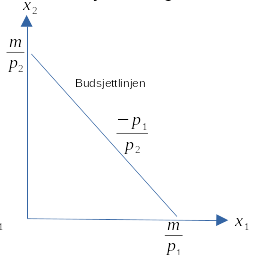
\includegraphics[width=1\textwidth,height=\textheight]{drawio/budsjbet.png}

}

\caption{Figur 7.7}

\end{figure}%

\begin{itemize}
\tightlist
\item
  Budsjettlinja viser alle kombinasjoner av \(x_1\) og \(x_2\) som
  konsumenten kan kjøpe, når hele inntekten brukes.
\end{itemize}

\begin{center}\rule{0.5\linewidth}{0.5pt}\end{center}

\subsubsection{Skjæringspunkter og
helning.}\label{skjuxe6ringspunkter-og-helning.}

Helningen på kurven er gitt ved (se appendisk for matetmatisk utledning)

\begin{equation}
\frac{\Delta x_{2}}{\Delta x_{1}}= - \frac{p_{1}}{p_{2}}
\end{equation}

Dersom vi kun velger \(x_1 \Rightarrow x_2=0\)

\begin{equation}
p_{1}x_{1}=m \\
x_{1} =m/p_{1}
\end{equation}

\textbf{Øvelse}: Hva skjer dersom vi kun velger \(x_2\)?

\begin{center}\rule{0.5\linewidth}{0.5pt}\end{center}

\textbf{Øvelse om budsjettlinjen}

Anta at du har en inntekt på 40 NOK som brukes på to goder. Gode 1
koster 10,- per enhet, og gode 2 koster 5,- per enhet.

\begin{enumerate}
\def\labelenumi{\arabic{enumi}.}
\tightlist
\item
  Skriv ned budsjettbetingelsen.
\item
  Hvor mye kan du kjøpe dersom du bruker all inntekten på gode 1?
\item
  Hvor mye kan du kjøpe dersom du bruker all inntekten på gode 2?
\item
  Tegn budsjettlinja.
\item
  Anta at prisen på gode 1 faller til 5 NOK. Skriv ned ny
  budsjettbetingelse. Tegn inn denne i diagrammet du brukte i forrige
  spørsmål
\end{enumerate}

\begin{center}\rule{0.5\linewidth}{0.5pt}\end{center}

\textbf{Svar vil bli lagt inn her}

\begin{itemize}
\tightlist
\item
  \begin{enumerate}
  \def\labelenumi{(\alph{enumi})}
  \tightlist
  \item
    Skriv ned budsjettbetingelsen. \begin{equation*}
    10x_{1}+5x_{2}=40
    \end{equation*}
  \end{enumerate}
\item
  \begin{enumerate}
  \def\labelenumi{(\alph{enumi})}
  \setcounter{enumi}{1}
  \tightlist
  \item
    Hvor mye kan du kjøpe dersom du bruker all inntekten på gode 1?
    \begin{equation*}
    x_{1} = \frac{40}{10} = 4
    \end{equation*}
  \end{enumerate}
\item
  \begin{enumerate}
  \def\labelenumi{(\alph{enumi})}
  \setcounter{enumi}{2}
  \tightlist
  \item
    Hvor mye kan du kjøpe dersom du bruker all inntekten på gode 2?
    \begin{equation*}
    x_{2} = \frac{40}{5} = 8
    \end{equation*}
  \end{enumerate}
\item
  \begin{enumerate}
  \def\labelenumi{(\alph{enumi})}
  \setcounter{enumi}{3}
  \tightlist
  \item
    Tegn budsjettlinja. Se diagramark
  \end{enumerate}
\item
  \begin{enumerate}
  \def\labelenumi{(\alph{enumi})}
  \setcounter{enumi}{4}
  \tightlist
  \item
    Anta at prisen på gode 1 faller til 5 NOK. Skriv ned ny
    budsjettbetingelse. Tegn inn denne i diagrammet du brukte i forrige
    spørsmål \begin{equation*}
    5x_{1}+5x_{2}=40
    \end{equation*}
  \end{enumerate}
\end{itemize}

\begin{center}\rule{0.5\linewidth}{0.5pt}\end{center}

\subsection{Konsumentens optimale
tilpasning}\label{konsumentens-optimale-tilpasning}

\begin{itemize}
\tightlist
\item
  Mål: tilpasse seg på høyest mulig nyttenivå for en gitt
  budsjettrestriksjon.
\item
  Altså: Nyttemaksimering.
\item
  Resultat: \begin{equation*}
  MSB=\frac{u'({x_{1}})}{u'({x_{2}})}=\frac{p_1}{p_2} \Leftrightarrow \\
  \frac{u'({x_{1}})}{p_{1}}=\frac{u'({x_{2}})}{p_{2}}
  \end{equation*}
\end{itemize}

\begin{center}\rule{0.5\linewidth}{0.5pt}\end{center}

\begin{itemize}
\tightlist
\item
  \emph{Gossens lov}: Nyttetilskuddet av den siste krona brukt på det
  ene godet, skal være lik Nyttetilskuddet av den siste krona brukt på
  det andre godet.
\end{itemize}

\begin{figure}[H]

{\centering 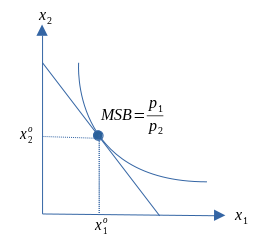
\includegraphics[width=1\textwidth,height=\textheight]{drawio/opttilp.png}

}

\caption{Figur 7.8}

\end{figure}%

\begin{center}\rule{0.5\linewidth}{0.5pt}\end{center}

\textbf{Øvelse (til neste forelesning) om konsumentens optimale
tilpasning}

Benytt opplysningene fra de to foregående øvelsene (øvelse om MSB og
budsjettlinjen), og skriv ned de to førsteordens betingelsene for
konsumentens optimale tilpasning. Illustrer så tilpasningen grafisk ved
bruk av et diagram.

\begin{center}\rule{0.5\linewidth}{0.5pt}\end{center}

\textbf{Svar:}

\begin{equation*}
MSB=\frac{x_2}{x_1} = 2  \\
10x_{1}+5x_{2}=40
\end{equation*} Vi kan løse det første uttrykket for \(x_2\)
\begin{equation*}
x_2 = 2x_1  \\
\end{equation*} Satt inn i budsjettbetingelsen og løst for \(x_1\)
\begin{equation*}
10x_{1}+5(2x{_1})=40 \Leftrightarrow
x_{1}=\frac{40}{20}=2
\end{equation*} Som deretter kan løses for \(x_2\) \begin{equation*}
x_2 = 2\cdot 2= 4  \\
\end{equation*}

\begin{center}\rule{0.5\linewidth}{0.5pt}\end{center}

\subsection{Appendiks}\label{appendiks-1}

\subsubsection{Matematisk utledning av helingen på
busjettkurven}\label{matematisk-utledning-av-helingen-puxe5-busjettkurven}

\begin{equation}
d(p_{1}x_{1}+p_{2}x_{2})=d(m)=0 \\
p_{1}\Delta x_{1}+p_{2}\Delta x_{2}  = 0 \\ 
p_{2}\Delta x_{2} =-p_{1}\Delta x_{1} \\
\frac{\Delta x_{2}}{\Delta x_{1}}= - \frac{p_{1}}{p_{2}}  \\ 
\end{equation}

\begin{center}\rule{0.5\linewidth}{0.5pt}\end{center}

\subsubsection{Matematisk utledning av
MSB}\label{matematisk-utledning-av-msb}

\begin{equation*}
U=u(x_{1}, x_{2})  \\
\text{Gitt nyttenivå} \\
\overline{U}=u(x_{1},x_{2}) \\ 
d\overline{U}=d(u(x_{1},x_{2})) \\
0 = u'_{x_{1}}\Delta x_{1}+u'_{x_{2}}\Delta x_{2} \\
-u'_{x_{2}}\Delta x_{2}  = u'_{x_{1}}\Delta x_{1}\\
-\Delta x_{2}/\Delta x_{1}  = \frac{u'_{x_{1}}}{u'_{x_{2}}}\\
MSB\equiv - \frac{\Delta x_{2}}{\Delta x_{1}}  = \frac{u'_{x_{1}}}{u'_{x_{2}}}
\end{equation*}

\begin{center}\rule{0.5\linewidth}{0.5pt}\end{center}

\subsubsection{Lagrange: Nyttemaksimering for et gitt
budsjett}\label{lagrange-nyttemaksimering-for-et-gitt-budsjett}

\textbf{Utledning: Løsning av nyttemaksimeringsproblemet ved bruk av
Lagrange-metode}

Maks \begin{equation*}
U=u(x_{1}, x_{2}) 
\end{equation*}

Gitt at

\begin{equation*}
p_{1}x_{1}+p_{2}x_{2}=m
\end{equation*}

Lagrangefunksjonen vil derfor være gitt ved \begin{equation*}
L = u(x_{1},x_{2}) - \lambda(p_{1}x_{1}+p_{2}x_{2}-m)
\end{equation*}

Første ordens betingelsene (indre løsning)

\begin{equation*}
L'_{x1}=u'({x_{1}}) - \lambda p_{1} = 0 \\
L'_{x2}=u'({x_{2}}) - \lambda p_{2} = 0 \\
p_{1}x_{1}+p_{2}x_{2}=m
\end{equation*}

\begin{center}\rule{0.5\linewidth}{0.5pt}\end{center}

Som gir oss to likninger til løsing av to ukjente, \(x_{1}\), \(x_{2}\):

\begin{equation*}
MSB=\frac{u'({x_{1}})}{u'({x_{2}})} = \frac{p_{1}}{p_{2}}  \\
p_{1}x_{1}+p_{2}x_{2}=m
\end{equation*}

Vi kan omskrive den første ligningen som (\emph{Gossens lov})

\begin{equation*}
\frac{u'({x_{1}})}{p_{1}}= \frac{u'({x_{2}})}{p_{2}}
\end{equation*}

Den rasjonelle konsument vil fordele utgiftene slik at den siste krone
gir den samme nyttendring uansett hvilket av de to godene den brukes til
innkjøp av.

class: inverse, center, middle

\section{Kapittel 8: Konsumentens økonomiske adferd i gode- og
arbeidsmarkedet}\label{kapittel-8-konsumentens-uxf8konomiske-adferd-i-gode--og-arbeidsmarkedet}

\begin{center}\rule{0.5\linewidth}{0.5pt}\end{center}

\subsection{Innledning}\label{innledning-2}

\begin{itemize}
\tightlist
\item
  Vi skal nå bruke det analyseapparatet vi har utviklet til å se på
  hvordan endringer i inntekt og priser vil virke inn på konsumentens
  konsummønster.
\item
  Vi skal også se hvordan vi kan bruke denne valghandlingsmodellen til

  \begin{itemize}
  \tightlist
  \item
    Utlede konsumentens etterspørselskurve etter goder.\\
  \item
    Utlede konsumentens tilbudskurve etter arbeid (ikke pensum)
  \end{itemize}
\end{itemize}

\begin{center}\rule{0.5\linewidth}{0.5pt}\end{center}

\subsection{Endring i pris og
priselastisitet}\label{endring-i-pris-og-priselastisitet}

\begin{itemize}
\tightlist
\item
  En prisendring vil endre helningen på budsjettlinja.
\item
  Når vi skal se på prisendringer er det viktig å skille mellom:
\item
  Egenprisvirkninger: endring i etterspørsel, ved endring i prisen på
  godet.
\item
  Kryssprisvirkninger: endring i etterspørsel, ved endring i prisen på
  det andre godet.
\end{itemize}

\begin{center}\rule{0.5\linewidth}{0.5pt}\end{center}

La oss stille følgende spørsmål: Dersom prisen på en vare reduseres med
10 kroner, og etterspurt kvantum øker med 100 enheter, er det mye eller
lite?

\begin{itemize}
\tightlist
\item
  Det relevante forholdet er \%-vis endring i etterspørsel, ved en
  \%-vis endring i pris. Det vil fortelle oss noe om prisfølsomheten.
\end{itemize}

Kvantumsendring i prosent: \begin{equation*}
\frac{\Delta X_{1}}{X_{1}}
\end{equation*}

Prisendring i prosent: \begin{equation*}
\frac{\Delta P_{1}}{P_{1}}
\end{equation*}

Elastisiteter: \begin{equation*}
e_{ij} \equiv \frac{\frac{\Delta X_{i}}{X_{i}}}{\frac{\Delta P{j}}{P_{j}}}=\frac{\Delta X_{i} P_{j} }{\Delta P_{j} X_{i}}
\end{equation*}

\begin{center}\rule{0.5\linewidth}{0.5pt}\end{center}

\subsubsection{Egenprisvirkninger}\label{egenprisvirkninger}

\begin{itemize}
\tightlist
\item
  Anta at \(p_1\) stiger. Hva skjer?
\item
  Budsjettrommet blir mindre ettersom budsjettlinja vris innover langs
  den horisontale aksen.

  \begin{itemize}
  \tightlist
  \item
    Normaltilfellet (vist i figur): pris og etterspørsel går motsatt
    vei. Økt pris fører til lavere etterspørsel, og motsatt.
  \item
    Giffen-tilfellet pris og etterspørsel går samme vei. Økt pris fører
    til økt etterspørsel, og motsatt.
  \end{itemize}
\end{itemize}

\begin{figure}[H]

{\centering 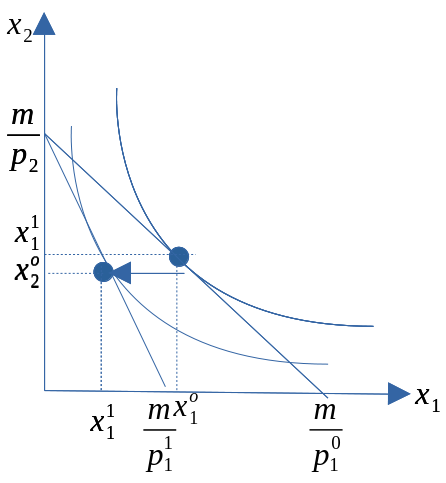
\includegraphics[width=1\textwidth,height=\textheight]{drawio/egenel.png}

}

\caption{Figur 8.1}

\end{figure}%

\begin{center}\rule{0.5\linewidth}{0.5pt}\end{center}

\textbf{Egenpriselastisitet}

\begin{itemize}
\tightlist
\item
  Egenpris-/Cournotelastisitet:

  \begin{itemize}
  \tightlist
  \item
    Viser \%-vis endring i etterspørselen etter gode \(x_1\) ved en
    endring i prisen på gode \(x_1\). (eventuelt for gode 2)
  \end{itemize}
\item
  Formelt: \begin{equation*}
  e_{11} \equiv \frac{\frac{\Delta X_{1}}{X_{1}}}{\frac{\Delta P_{1}}{P_{1}}}=\frac{\Delta X_{1} P_{1} }{\Delta P_{1} X_{1}}
  \end{equation*}

  \begin{itemize}
  \tightlist
  \item
    \(e_{11} < -1\): Priselastisk
  \item
    \(e_{11} = -1\): Prisnøytralt
  \item
    \(-1< e_{11}< 0\): Prisuelastisk
  \item
    \(e_{11} > 0\): (Giffen-gode)
  \end{itemize}
\end{itemize}

\begin{center}\rule{0.5\linewidth}{0.5pt}\end{center}

\subsubsection{Kryssprisvirkninger}\label{kryssprisvirkninger}

Hva skjer med etterspørselen etter \(x_2\) når prisen på gode \(x_1\)
øker? Det kan i utgangspunktet skje tre ting.

\begin{itemize}
\tightlist
\item
  Etterspørselen etter gode \(x_2\) øker. Erstatter bort \(x_1\) til
  fordel for \(x_2\).

  \begin{itemize}
  \tightlist
  \item
    \(\Rightarrow\) Alternative goder
  \end{itemize}
\item
  Etterspørselen etter gode \(x_2\) reduseres (vist i figur). Kjøper
  altså mer av både \(x_1\) og \(x_2\)

  \begin{itemize}
  \tightlist
  \item
    \(\Rightarrow\) Komplementære goder
  \end{itemize}
\item
  Etterspørselen etter gode \(x_2\) påvirkes ikke.

  \begin{itemize}
  \tightlist
  \item
    \(\Rightarrow\) Godene er uavhengige av hverandre
  \end{itemize}
\end{itemize}

\begin{center}\rule{0.5\linewidth}{0.5pt}\end{center}

\begin{figure}[H]

{\centering 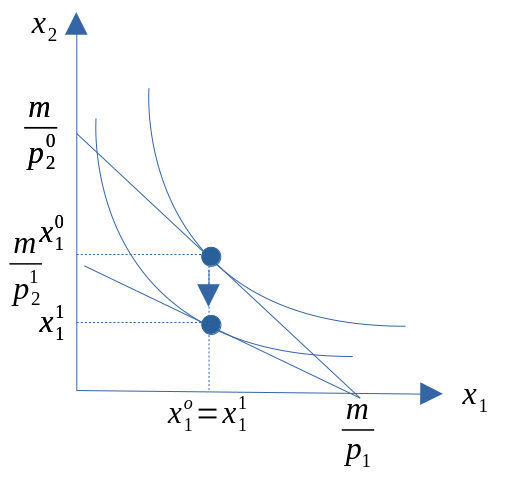
\includegraphics[width=1\textwidth,height=\textheight]{drawio/kryssel.png}

}

\caption{Figur 8.2}

\end{figure}%

\begin{center}\rule{0.5\linewidth}{0.5pt}\end{center}

\textbf{Krysspriselastisitet}

\begin{itemize}
\tightlist
\item
  Viser \%-vis endring i etterspørselen etter gode \(x_1\), ved en
  endring i prisen på gode \(x_2\). Eller motsatt.
\item
  Formelt: \begin{equation*}
  e_{12} \equiv \frac{\frac{\Delta X_{1}}{X_{1}}}{\frac{\Delta P_{2}}{P_{2}}}=\frac{\Delta X_{1} P_{2} }{\Delta P_{2} X_{1}}
  \end{equation*}

  \begin{itemize}
  \tightlist
  \item
    \(e_{12} < 0\): Komplementært til \(x_2\)
  \item
    \(e_{12} > 0\): Alternativ til \(x_2\)
  \item
    \(e_{12} = 0\): Uavhengig av \(x_2\)
  \end{itemize}
\end{itemize}

\begin{center}\rule{0.5\linewidth}{0.5pt}\end{center}

\subsubsection{Inntektsendringer}\label{inntektsendringer}

\begin{itemize}
\tightlist
\item
  En endring i konsumentens inntekt vil føre til at budsjettlinja
  parallellforskyves.
\item
  Merk forskjellen mellom normalgoder og mindreverdige goder.
\item
  Dersom vi trekker en linje gjennom de optimale godekombinasjoner, får
  vi en kurve som kalles inntekts-forbrukskurven (Engel-kurven).
\end{itemize}

\begin{figure}[H]

{\centering 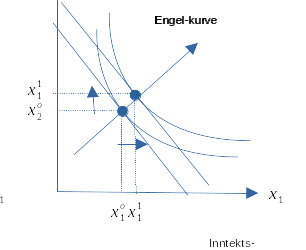
\includegraphics[width=1\textwidth,height=\textheight]{drawio/inntel.png}

}

\caption{Figur 8.3}

\end{figure}%

\begin{center}\rule{0.5\linewidth}{0.5pt}\end{center}

\textbf{Inntektselastisitet} - Viser hvor mye etterspørselen endres, ved
en liten endring i inntekt. - Formelt. \begin{equation*}
E_1 \equiv \frac{\frac{\Delta X_{1}}{X_{1}}}{\frac{\Delta Y}{Y}}=\frac{\Delta X_{1} Y }{\Delta Y X_{1}}
\end{equation*}

\begin{itemize}
\tightlist
\item
  \(E_1 > 1\): Inntektselastisk gode
\item
  \(E_1 = 1\): Inntektsnøytralt gode
\item
  \(0 < E_1 < 1\): Inntektsuelastisk gode
\item
  \(E_1 < 0\): Mindreverdig gode
\item
  \(E_1 > 0\): Nøytralt gode
\end{itemize}

\begin{center}\rule{0.5\linewidth}{0.5pt}\end{center}

\subsection{Dekomponering av virkningen av prisendringer: Substitusjons-
og
inntektsvirkning}\label{dekomponering-av-virkningen-av-prisendringer-substitusjons--og-inntektsvirkning}

\begin{itemize}
\tightlist
\item
  Vi har sett hvordan prisendringer kan påvirke konsumet. Vi skal nå
  splitte denne totale priseffekten opp i to virkninger:
\item
  Substitusjonsvirkning
\item
  Den effekt på konsumet som oppstår som følge av en endring i det
  relative prisforholdet ( \(\frac{p_1}{p_2}\) ). Dette krever at
  konsumenten får en inntektskompensasjon for realinntektstapet.
  \(\Rightarrow\) Nyttenivået opprettholdes.
\end{itemize}

\begin{center}\rule{0.5\linewidth}{0.5pt}\end{center}

\begin{itemize}
\tightlist
\item
  Inntektseffekten

  \begin{itemize}
  \tightlist
  \item
    Anta nå at vi ser bort i fra inntektskompensasjonen og tar hensyn
    til at økt \(p_1\) vil redusere realinntekten. Den virkningen som
    oppstår på konsumet som følge av endringen i realinntekt, kalles
    inntektseffekten. Denne vil parallellforskyve budsjettlinja, uten at
    helningen endres.
  \end{itemize}
\item
  Totaleffekten

  \begin{itemize}
  \tightlist
  \item
    Substitusjonseffekt + inntektseffekt = Priseffekt
  \end{itemize}
\end{itemize}

\begin{figure}[H]

{\centering 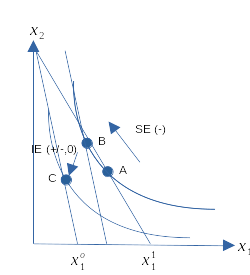
\includegraphics[width=0.4\textwidth,height=\textheight]{drawio/utletter.png}

}

\caption{Figur 8.4}

\end{figure}%

\begin{center}\rule{0.5\linewidth}{0.5pt}\end{center}

\subsection{Fra optimal tilpasning til
etterspørsel}\label{fra-optimal-tilpasning-til-etterspuxf8rsel}

\begin{itemize}
\tightlist
\item
  Fra teorien over kan vi utlede konsumentens etterspørselsfunksjon og
  etterspørselskurve.
\item
  Merk: Fra optimeringsproblemet har vi to betingelser som må være
  oppfylt: tangeringsbetingelsen og budsjettbetingelsen. Vi har også to
  ukjent. De kjente størrelsen som bestemmer disse to er prisene og
  inntekten. Altså blir de to ukjente funksjoner av priser og inntekt.
  Vi kan dermed skrive etterspørselsfunksjonene som:

  \begin{itemize}
  \tightlist
  \item
    \(x_1^D=D(p_1,p_2,m)\)
  \item
    \(x_2^D=D(p_1,p_2,m)\)
  \end{itemize}
\end{itemize}

\begin{center}\rule{0.5\linewidth}{0.5pt}\end{center}

\subsubsection{Etterspørselskurven}\label{etterspuxf8rselskurven}

\begin{itemize}
\tightlist
\item
  Denne viser sammenhengen mellom prisen på et gode og etterspurt
  kvantum etter godet.
\item
  Basert på etterspørselsfunksjonene holder vi dermed prisen på gode 2
  og inntekten konstant. Etterspørselen etter gode 1 kan da skrives:
  \begin{equation*}
  x_{1}^{D}=D(p_1)
  \end{equation*}
\item
  Vi tar utgangspunkt i konsumentens optimale tilpasning, og antar så
  prisøkninger på gode \(x_1\).
\end{itemize}

\begin{figure}[H]

{\centering 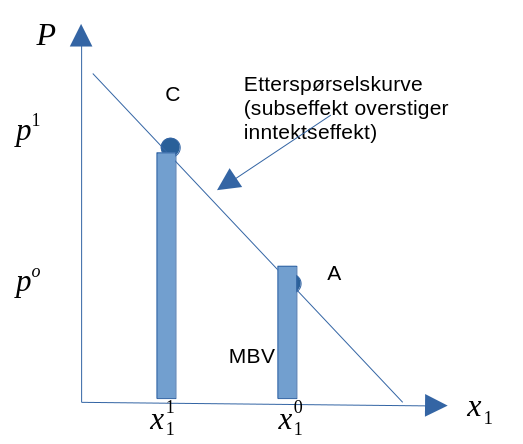
\includegraphics[width=0.4\textwidth,height=\textheight]{drawio/ekonsum.png}

}

\caption{Figur 8.5}

\end{figure}%

\begin{itemize}
\tightlist
\item
  Kurven har negativ helning: \(\frac{dx_1^D}{dp_1}<0\) (gjelder alltid,
  bortsett fra i Giffen-tilfellet).
\end{itemize}

\begin{center}\rule{0.5\linewidth}{0.5pt}\end{center}

\subsubsection{Tilbudsfunksjonen etter
arbeid}\label{tilbudsfunksjonen-etter-arbeid}

Budsjettbetingelsen \begin{equation*}
px = wN\\
N = M-L \\
px = w(M-L) \\
px =wM -wL \\
px+wL = wM  
\end{equation*}

Nyttefunksjonen består derfor av konsumgode (x) og fritid (L)

\begin{equation*}
U=u(x,L) \text{ } u^{'}_{x} >0, u^{''}_{x} <0, u^{'}_{L} >0, u^{''}_{L} <0
\end{equation*}

\begin{center}\rule{0.5\linewidth}{0.5pt}\end{center}

\textbf{Optimal tilpasning}

\begin{figure}[H]

{\centering 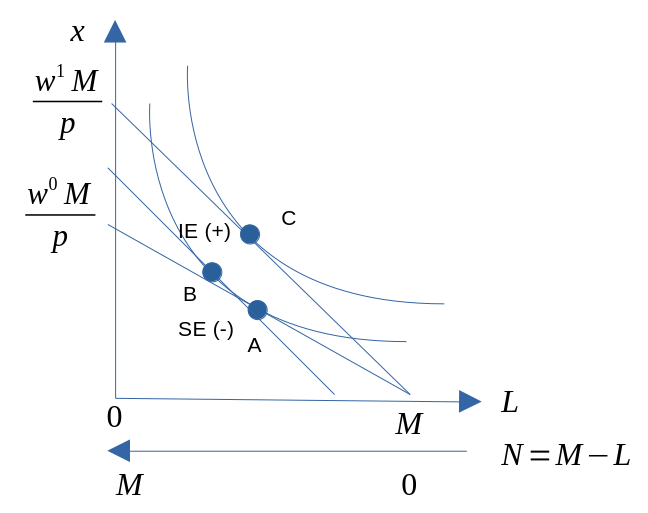
\includegraphics[width=1\textwidth,height=\textheight]{drawio/utltilbud.png}

}

\caption{Figur 8.6}

\end{figure}%

\begin{center}\rule{0.5\linewidth}{0.5pt}\end{center}

\textbf{Husholdningens tilbud av arbeidskraft}

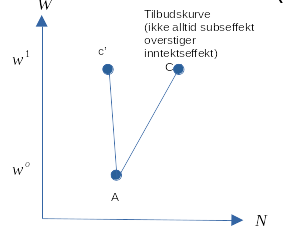
\includegraphics[width=1\textwidth,height=\textheight]{drawio/tarbeid.png}

\begin{center}\rule{0.5\linewidth}{0.5pt}\end{center}

\subsection{Appendiks}\label{appendiks-2}

\textbf{Løsningsforslag}

Optimal løsning er kjennetegnet ved \begin{equation*}
MSB = \frac{p_{1}}{p_{2}}\\
p_{1}x_{1}+p_{2}x_{2}= m 
\end{equation*}

Som gir oss \begin{equation*}
MSB = \frac{U'_{1}}{U'_{2}}= \frac{1+x_{2}}{1+x_{1}} = \frac{p_{1}}{p_{2}}\\
p_{2}x_{2} =p_1+p_1x_1-p_2 \\ 
\text{I budsjettbetingelsen kan vi sette inn for } p_{2}x_{2} \\
R=p_1x_1+p_1+p_1x_1-p_2\\
2p_{1}x_{1} = R-p_1+p_2 \\
\text{Som gir oss etterspørselsfunksjonen}  \\
x_{1} = \frac{R-p_1+p_2}{2p_{1}}   \\ 
\end{equation*}

\begin{center}\rule{0.5\linewidth}{0.5pt}\end{center}

\begin{enumerate}
\def\labelenumi{\alph{enumi})}
\setcounter{enumi}{1}
\tightlist
\item
  Med \emph{normalt gode} menes goder hvor etterspørselen øker når
  inntekten øker. For \emph{mindreverdige goder} gjelder det motsatte.
  \begin{equation*}
  \frac{\partial  x_{1}}{\partial R} = \frac{1}{2p_1} > 0 \text{ dvs. normal gode}
  \end{equation*}
\item
  For \emph{komplementære goder} vil etterspørselen etter gode reduseres
  når prisen på det andre goder øker. For \emph{alternative} goder
  gjelder det motsatte. \begin{equation*}
  \frac{\partial  x_{1}}{\partial p_{2}} = \frac{1}{2p_1}  > 0 \text{ dvs. alternative goder}
  \end{equation*}
\end{enumerate}

\begin{center}\rule{0.5\linewidth}{0.5pt}\end{center}

class: inverse, center, middle

\section{Kapittel 9: Markedsteori: Fullkommen
konkurranse}\label{kapittel-9-markedsteori-fullkommen-konkurranse}

\begin{center}\rule{0.5\linewidth}{0.5pt}\end{center}

\subsection{Innledning}\label{innledning-3}

\begin{itemize}
\tightlist
\item
  Vi begynte dette kurset med å se på markedsformen fullkommen
  konkurranse. Vi skal nå se nærmere på denne.
\item
  Spesielt skal vi se på:
\item
  Forutsetningene som markedsformen bygger på.
\item
  Samfunnsøkonomisk overskudd (lønnsomhet) i forbindelse med denne måten
  å organisere markedet på.
\item
  Gjennom de foregående kapitlene har vi lært masse om konsumenter og
  produsenter hver for seg. Poenget i markedsteorien er å studere
  hvordan disse aktørene opptrer på en markedsplass.
\item
  Vi skal anta at interaksjonen skjer på et varemarked der konsumentene
  etterspør varer, og produsentene tilbyr varer.
\item
  Det finnes flere måter å organisere en markedsøkonomi på. Avhenger av
  varen som omsettes, antall aktører med mer.
\end{itemize}

\begin{center}\rule{0.5\linewidth}{0.5pt}\end{center}

\subsubsection{Forutsetninger}\label{forutsetninger}

\begin{enumerate}
\def\labelenumi{\arabic{enumi}.}
\tightlist
\item
  Mange aktører på tilbudssiden og etterspørselssiden. Kan ikke alene
  påvirke prisene. Betraktes derfor som gitt.
\item
  Prisene blir bestemt i et samspill mellom tilbydere og etterspørrere.
\item
  Homogene (identiske) varer.
\item
  Rasjonelle aktører: Konsumentene maksimerer nytte og produsentene
  maksimerer fortjeneste.
\item
  Full informasjon om alle relevante forhold.
\item
  Alle kan kostnadsfritt gå inn og ut av markedet.
\end{enumerate}

\begin{center}\rule{0.5\linewidth}{0.5pt}\end{center}

\subsubsection{Markedslikevekt}\label{markedslikevekt-1}

\begin{itemize}
\tightlist
\item
  Markedstilbud: vi har allerede sett hvordan tilbudskurven er stigende
  i et pris-mengde diagram.

  \begin{itemize}
  \tightlist
  \item
    MERK: Vi nå kan forklare dette med stigende grensekostnadskurve.
  \end{itemize}
\item
  Markedsetterspørsel: som vi har sett er etterspørselskurven fallende i
  et pris-mengde diagram.

  \begin{itemize}
  \tightlist
  \item
    MERK: at vi nå kan forklare det med utgangspunkt i konsumentens
    optimale tilpasning på varemarkedet.
  \end{itemize}
\end{itemize}

\begin{figure}[H]

{\centering 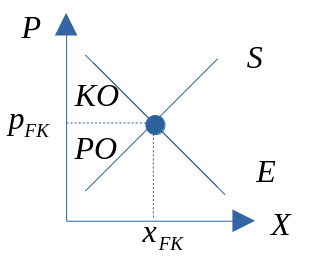
\includegraphics[width=0.4\textwidth,height=\textheight]{drawio/markl.png}

}

\caption{Figur 9.1}

\end{figure}%

\begin{center}\rule{0.5\linewidth}{0.5pt}\end{center}

\subsection{Velferdsøkonomi og samfunnsøkonomisk
overskudd}\label{velferdsuxf8konomi-og-samfunnsuxf8konomisk-overskudd}

\begin{itemize}
\tightlist
\item
  I samfunnsøkonomi er vi naturlig nok opptatt av å vurdere om et marked
  eller et prosjekt eller politikkforslag er samfunnsøkonomisk lønnsomt.
  Når alt kommer til alt er det jo høyest mulig velferd for individene i
  samfunnet som er målet.
\item
  For å vurdere velferden brukes begrepet samfunnsøkonomisk overskudd
  (SO).
\item
  Dette består av konsumentoverskudd (KO) og produsentoverskudd (PO)
\item
  Vi har derfor at: \begin{equation*}
  SO=PO+KO
  \end{equation*}
\end{itemize}

\begin{center}\rule{0.5\linewidth}{0.5pt}\end{center}

\subsection{Konsumentoverskudd}\label{konsumentoverskudd-1}

\subsubsection{Betalingsvillighet}\label{betalingsvillighet}

\begin{itemize}
\tightlist
\item
  I konsumentteorien var vi opptatt av å maksimere nytte. Men hvordan
  måle nytte? Hvor mye du er villig til å betale for en vare kan
  fortelle noe om nytten du oppnår. Det kalles:

  \begin{itemize}
  \tightlist
  \item
    Betalingsvillighet: \(B\)
  \end{itemize}
\item
  Betalingsvilligheten avhenger av hvor mye du har i utgangspunktet:
  \(\Rightarrow B(X)\)
\end{itemize}

\begin{center}\rule{0.5\linewidth}{0.5pt}\end{center}

\subsubsection{Den marginale
betalingsvillighet}\label{den-marginale-betalingsvillighet}

\begin{itemize}
\tightlist
\item
  For å finne et uttrykk for hvor mye du vil betale for en ekstra enhet
  kan vi derivere \(B\). Det gir: \(B’(X)\), som kalles den marginal
  betalingsvillighet. Merk: Avhenger også av \(X\).
\item
  Videre vet vi at etterspørselskurven viser hvor mange enheter
  konsumenten er villig til å kjøpe ved ulike priser. Dvs. at på kurven
  måles endring i etterspørsel ved liten endring i pris. Dette må
  sammenfalle med marginal betalingsvillighet.
\item
  Betalingsvilligheten blir da området under E-kurven.
\end{itemize}

\begin{figure}[H]

{\centering 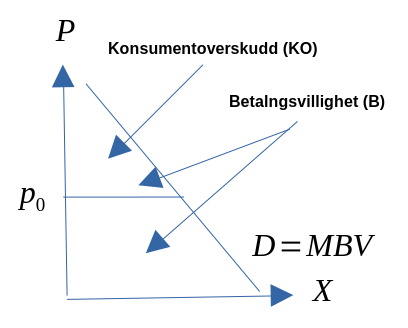
\includegraphics[width=0.4\textwidth,height=\textheight]{drawio/konso.png}

}

\caption{Figur 9.2}

\end{figure}%

\begin{center}\rule{0.5\linewidth}{0.5pt}\end{center}

\subsubsection{Sammenhengen mellom betalingsvillighet og
konsumentoverskuddet}\label{sammenhengen-mellom-betalingsvillighet-og-konsumentoverskuddet}

\begin{itemize}
\tightlist
\item
  Det et imidlertid forskjell på det konsumenten er villig til å betale,
  og det han faktisk betaler. Det er denne differensen som er
  konsumentoverskuddet:

  \begin{itemize}
  \tightlist
  \item
    \(\Rightarrow KO(X) = B(X) – pX\)
  \end{itemize}
\item
  Merk at \(B(X)\) her viser betalingsvillighet for \(X\) enheter. Det
  konsumentene faktisk må betale for dette antallet er \(pX\). Ettersom
  begge disse leddene avhenger av \(X\), må også konsumentoverskuddet
  gjøre det, \(KO(X)\).
\item
  Optimal tilpasning for konsumenten viser det optimale antall enheter
  konsumenten vil kjøpe dersom han/hun maksimerer konsumentoverskuddet.
  Finner 1.ordensbetingelsen: \begin{equation*}
  KO’(X) = B’(X) – p = 0 \Leftrightarrow B’(X) = p
  \end{equation*}
\item
  Denne betingelsen bestemmer optimal \(X\). Altså: når det konsumenten
  betaler for siste enhet, er lik det konsumenten ønsker å betale for
  denne enheten.
\end{itemize}

\begin{center}\rule{0.5\linewidth}{0.5pt}\end{center}

\subsection{Produsentoverskudd}\label{produsentoverskudd-1}

\begin{itemize}
\tightlist
\item
  I produksjonsteorien var vi blant annet opptatte av at bedriftene
  maksimerer fortjeneste. Dette er enkelt å måle som differensen mellom
  inntekter og utgifter.
\item
  Produsentoverskudd defineres som summen av den ekstrainntekten som
  produsenten får, av å selge til en pris som er høyere enn den laveste
  de ville vært villige til å akseptere.
\item
  Det vil si: differensen mellom produsentens samlede salgsinntekter og
  variable kostnader.
\end{itemize}

\begin{figure}[H]

{\centering 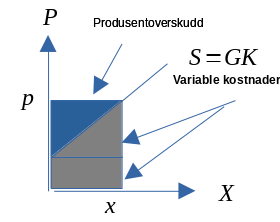
\includegraphics[width=0.4\textwidth,height=\textheight]{drawio/prodo.png}

}

\caption{Figur 9.3}

\end{figure}%

\begin{center}\rule{0.5\linewidth}{0.5pt}\end{center}

\subsubsection{Sammenhengen mellom salgsinntekt og
produsentoverskudd}\label{sammenhengen-mellom-salgsinntekt-og-produsentoverskudd}

\begin{itemize}
\tightlist
\item
  Altså: \begin{equation*}
  PO(X) = pX – CV(X)
  \end{equation*}
\item
  Naturlig nok vil produsentene maksimere PO. Vi finner
  1.ordensbetingelsen: \begin{equation*}
  PO’(X) = p – C’(X) = 0 \Leftrightarrow p = C’(X)
  \end{equation*}
\item
  De tilpasser kvantumet slik at kostnaden ved siste produserte enhet er
  lik prisen.
\item
  Grafisk fremstilling av PO: tar utgangspunkt i tilbudskurven.
  Tilbudskurven viser hvor mange enheter som vil tilbys dersom prisen
  f.eks. er \(p_1\).
\item
  For en gitt pris kan vi lese av inntekten og samlet merkostnad.
\item
  PO fremkommer som området mellom prislinja og tilbudskurven.
\end{itemize}

\begin{center}\rule{0.5\linewidth}{0.5pt}\end{center}

\subsection{Samfunnsøkonomisk overskudd og fullkommen
konkurranse}\label{samfunnsuxf8konomisk-overskudd-og-fullkommen-konkurranse-1}

\begin{itemize}
\item
  Vi har nå sett at konsumentene velger sitt konsum slik at
  \(B’(X) = p\), og produsentene velger sitt produksjonskvantum slik at
  \(p = C’(X)\).
\item
  Maksimalt SO finner vi ved \begin{equation*}
  \underset{X}{\text{Maks}SO}=PO+KO=(pX-CV(x))+(B(x)-pX)
  \end{equation*} Som gir oss følgende 1.ordensbetingelse:
  \begin{equation*}
  SO’(X) = KO’(X) + PO’(X) = 0 \\
  \Rightarrow SO’(X) = B’(X) – p + p – C’(X) = 0\\
  \Rightarrow SO’(X) = B’(X) – C’(X) = 0 \\
  \Leftrightarrow B’(X) = C’(X)
  \end{equation*} ---
\item
  Er denne betingelsen tilfredsstilt i fullkommen konkurranse? JA!
\end{itemize}

\emph{Sosial planlegger}

\includegraphics[width=0.45\textwidth,height=\textheight]{drawio/planl.png}

\emph{Fullkommen konkurranse}

\includegraphics[width=0.45\textwidth,height=\textheight]{drawio/markl.png}

\begin{itemize}
\tightlist
\item
  Ettersom konsumenter og produsenter tilpasser seg de samme prisene,
  altså p = p.~Vi ser da at \(B’(X) = C’(X)\), som er kravet til
  maksimalt SO.

  \begin{itemize}
  \tightlist
  \item
    Fullkommen konkurranse gir altså maksimalt samfunnsøkonomisk
    overskudd.
  \end{itemize}
\end{itemize}

\begin{center}\rule{0.5\linewidth}{0.5pt}\end{center}

\subsection{Avgift og velferd}\label{avgift-og-velferd}

\begin{itemize}
\tightlist
\item
  Hva skjer med det samfunnsøkonomiske overskuddet ved innføring av en
  avgift?
\item
  Vi har allerede sett at avgiften fører til en ``glippe'' eller en
  ``kile'' mellom den prisen som produsenten mottar, og den prisen som
  konsumenten betaler.
\end{itemize}

\begin{figure}[H]

{\centering \includegraphics[width=0.35\textwidth,height=\textheight]{drawio/avgfk.png}

}

\caption{Figur 9.4}

\end{figure}%

\begin{itemize}
\tightlist
\item
  Av analysen kommer det frem at tapet til konsumenten og produsenten er
  større enn gevinsten til myndighetene. Denne reduksjonen i det
  samfunnsøkonomiske overskuddet kalles for dødvektstap eller
  effektivitetstap.
\end{itemize}

\begin{center}\rule{0.5\linewidth}{0.5pt}\end{center}

\textbf{Øvelse}

\begin{itemize}
\tightlist
\item
  Etterspørsel (MBV): \(P = 20 – X\). Tilbud (GK): \(P = 2 + 2X\)

  \begin{enumerate}
  \def\labelenumi{\alph{enumi}.}
  \tightlist
  \item
    Finn likevektspris, omsatt kvantum og vis tilpasningen grafisk.
  \item
    Regn ut KO, PO og SO.
  \item
    Det innføres en skatt på 3 kroner per produserte enhet. Sett opp ny
    tilbudsfunksjon og regn ut \(P_K\) (pris til konsument), \(P_P\)
    (pris til produsent) og omsatt kvantum \(X\).
  \item
    Hva blir KO, PO nå?
  \item
    Regn ut avgiftsinntekten for staten og effektivitetstapet (antar her
    at skatteinntektene blir betalt tilbake igjen til både konsument og
    produsent)..
  \end{enumerate}
\end{itemize}

\begin{center}\rule{0.5\linewidth}{0.5pt}\end{center}

\textbf{Løsningsforslag}

\begin{enumerate}
\def\labelenumi{\alph{enumi})}
\tightlist
\item
  Vi starter med omsatt kvantum. I fullkommen vil løsningen være
  karakterisert ved at MBV=GK, det gir oss \begin{equation*}
  20-x=2+2x \\
  -x-2x =2-20 \\
  3x   =18 \\
  x^{FK}=x =\frac{18}{3} = 6
  \end{equation*} Setter vi dette kvantumet inn i enten etterspørs-
  eller tilbudskurven vil vi finne produktprisen \begin{equation*}
  x = 6 \\
  MBV: P = 20-6=14 \\
  (GK: P = 2+26 = 14)
  \end{equation*}
\end{enumerate}

\begin{center}\rule{0.5\linewidth}{0.5pt}\end{center}

\begin{enumerate}
\def\labelenumi{\alph{enumi})}
\setcounter{enumi}{1}
\tightlist
\item
  Konsumentoverskuddet er gitt ved arealet til trekanten
  \begin{equation*}
  KO = (6-0)\cdot(20-14)/2 = 18
  \end{equation*} Mens produsentoverskudet er gitt ved \begin{equation*}
  PO = (6-0)(14-2)/2 = 36
  \end{equation*} Samfunnsøkonomisk overskudd blir derfor
  \begin{equation*}
  SO = PO+KO =36+18=54
  \end{equation*}
\end{enumerate}

\begin{center}\rule{0.5\linewidth}{0.5pt}\end{center}

\begin{enumerate}
\def\labelenumi{\alph{enumi})}
\setcounter{enumi}{2}
\tightlist
\item
\end{enumerate}

Skatt per enhet gjør at tilbudskurven kan skrives som \begin{equation*}
P = 2+2x + 3 \\
20-x=2+2x+3 \\
3x   =15 \\
x = 5
\end{equation*} Prisen til konsument blir derfor \begin{equation*}
P_k = 20 - 5 = 15
\end{equation*} Mens pris til produsent blir \begin{equation*}
P_p=2+2\cdot5 = 2+10 = 12
\end{equation*}

\begin{center}\rule{0.5\linewidth}{0.5pt}\end{center}

\begin{enumerate}
\def\labelenumi{\alph{enumi})}
\setcounter{enumi}{3}
\tightlist
\item
  Konsument- , produsentoverskudd og samfunnsøkonomisk overskudd er nått
  gitt ved \begin{equation*}
  KO = \frac{(5\cdot (20-15))}{2}  = 12.5\\
  PO = \frac{(5\cdot (12-2))}{2} = 25
  \end{equation*}
\end{enumerate}

\begin{center}\rule{0.5\linewidth}{0.5pt}\end{center}

\begin{enumerate}
\def\labelenumi{\alph{enumi})}
\setcounter{enumi}{4}
\tightlist
\item
\end{enumerate}

Avgiftsinntekten (SI) og Dødvektstapet (DT): \begin{equation*}
SI = (5-0)(15-12)= 15 \\
DT =\frac{((6-5))(15-12)}{2} = \frac{1 \cdot 3}{2} = 1.5 \\
SO (\text{med tilbakebetaling av SI til KO og PO})= 12.5+25 + 15 =  37.5 + 15 = 52.5
\end{equation*}

\begin{center}\rule{0.5\linewidth}{0.5pt}\end{center}

\subsection{Elastisiteter, avgifter og
velferdsøkonomi}\label{elastisiteter-avgifter-og-velferdsuxf8konomi}

\begin{itemize}
\tightlist
\item
  En mer horisontal (vertikal) etterspørselkurve innebærer en mer
  prisfølsom/elastisk (uelastisk) etterspørsel.
\item
  Ved skiftanalsye

  \begin{itemize}
  \tightlist
  \item
    Større (mindre) effekt på produksjonen
  \end{itemize}
\item
  Ved en avgift, vil dette innebære at:

  \begin{itemize}
  \tightlist
  \item
    Dødvektstap blir større (mindre)
  \item
    En større (mindre) andel av avgiftsinntektene blir betalt av
    produsenten
  \end{itemize}
\end{itemize}

\begin{center}\rule{0.5\linewidth}{0.5pt}\end{center}

\begin{itemize}
\tightlist
\item
  En mer horisontal (vertikal) tilbudskurve innebærer en mer
  prisfølsom/elastisk (uelastisk) tilbud.
\item
  Ved skiftanalsye

  \begin{itemize}
  \tightlist
  \item
    Større (mindre) effekt på produksjonen
  \end{itemize}
\item
  Ved en avgift, vil dette innebære at:

  \begin{itemize}
  \tightlist
  \item
    Dødvektstap blir større (mindre)
  \item
    En større (mindre) andel av avgiftsinntektene blir betalt av
    konsumenten.
  \end{itemize}
\end{itemize}

\begin{center}\rule{0.5\linewidth}{0.5pt}\end{center}

\textbf{Øvelse}

\begin{itemize}
\tightlist
\item
  Forsøk å illustrer disse resultatene grafisk ved bruk av diagrammer.
\end{itemize}

\begin{center}\rule{0.5\linewidth}{0.5pt}\end{center}

\subsubsection{Appendiks
(Prismekanismen)}\label{appendiks-prismekanismen}

\textbf{Friedman om prismekanismen (kort versjon)}

\url{https://www.youtube.com/watch?v=R5Gppi-O3a8}

\textbf{Friedman om prismekanismen (lengre versjon)}

\url{https://www.youtube.com/watch?v=4ERbC7JyCfU&t=3s}

\section{Kapittel 10: Markedsteori: Ufullkommen konkurranse -
Monopol}\label{kapittel-10-markedsteori-ufullkommen-konkurranse---monopol}

\begin{center}\rule{0.5\linewidth}{0.5pt}\end{center}

\subsection{Innledning}\label{innledning-4}

\begin{itemize}
\tightlist
\item
  Vi skal her se nærmere på følgende:

  \begin{enumerate}
  \def\labelenumi{\arabic{enumi}.}
  \tightlist
  \item
    Årsaker til monopol
  \item
    Monopolistens tilpasning
  \item
    Samfunnsøkonomisk overskudd under monopol
  \end{enumerate}
\item
  Ved monopol antas det fremdeles mange kjøpere, men bare én tilbyder.
\item
  Det å være en gir bedriften økt kontroll mht. pris og
  produksjonsmengde.
\item
  Merk imidlertid at bedriften må ta hensyn til konsumentenes
  etterspørsel, slik at helt fritt kan den ikke tilpasse seg.
\item
  Begrensningen for monopolisten ligger altså i hva folk ønsker seg, og
  hvor mye de er villige til å betale.
\item
  Men konkurranse fra andre (tilbydere) slipper monopolisten (pr.
  definisjon).
\end{itemize}

\begin{center}\rule{0.5\linewidth}{0.5pt}\end{center}

\subsection{Årsaker til monopol}\label{uxe5rsaker-til-monopol}

\begin{itemize}
\item
  For at et monopol skal kunne opprettholdes over tid, må det eksistere
  en form for \emph{etableringshinder} i markedet.
\item
  Ved et monopol har produsenten større kontroll over prisen (prislager
  eller «pricemaker»), dette skaper en genuin profittmulighet.
\item
  Profittmuligheten vil i utgangspunktet trekke til seg andre
  konkurrenter, men markedshindrene gjør dette umulig.
\item ~
  \subsection{Merk at dette skiller monopolet fra den enkelte bedrift i
  fullkommen konkurranse, som sies å være pristaker
  (pricetaker).}\label{merk-at-dette-skiller-monopolet-fra-den-enkelte-bedrift-i-fullkommen-konkurranse-som-sies-uxe5-vuxe6re-pristaker-pricetaker.}
\end{itemize}

\subsection{Etableringshindre}\label{etableringshindre}

\begin{itemize}
\tightlist
\item
  Forbud mot nyetableringer: postverket, vinmonopolet.
\item
  Patentrettigheter eller vanlige rettigheter: eksklusiv rettighet på
  produkt eller produksjonsteknikk.
\item
  Kontroll over sentrale produksjonsfaktorer/råvarer.
\item
  Lokale markeder: butikker som ligger i betydelig avstand til
  konkurrenter.
\item
  Stordriftsfordeler. Innebærer fallende enhetskostnader: jernbane
  (NSB).
\end{itemize}

\begin{center}\rule{0.5\linewidth}{0.5pt}\end{center}

\subsection{Monopolistens tilpasning}\label{monopolistens-tilpasning}

\subsubsection{Monopolistens tilpasning: intuitiv
forklaring}\label{monopolistens-tilpasning-intuitiv-forklaring}

\begin{itemize}
\item
  Det er naturlig å anta at monopolisten vil maksimere fortjenesten.
  Spørsmålet er hvilket kvantum som gir maksimal fortjeneste.
\item
  Svaret er: bedriften vil produsere inntil inntekten ved å produsere en
  ekstra enhet er lik kostnaden ved å produsere en enhet til.
\item
  Inntekten (merk at det står inntekt og ikke profitt) bedriften får ved
  å produsere og selge en enhet til kalles grenseinntekten, R'(X).
\item ~
  \subsection{Kostnaden ved å produsere en enhet til kjenner vi som
  grensekostnaden,
  C'(X).}\label{kostnaden-ved-uxe5-produsere-en-enhet-til-kjenner-vi-som-grensekostnaden-cx.}
\item
  Altså blir betingelsen for optimal produksjon:
\item
  \(R’(X) = C’(X)\)
\item
  Du kan lettere se at det må være slik dersom du prøver deg med å anta
  at betingelsen ikke er oppfylt.

  \begin{itemize}
  \tightlist
  \item
    Hvis \(R’(X) > C’(X)\) vil overskuddet øke ved økt produksjon og
    salg.
  \item
    Hvis \(R’(X) < C’(X)\) vil overskuddet øke ved redusert produksjon
    og salg.
  \end{itemize}
\end{itemize}

\begin{center}\rule{0.5\linewidth}{0.5pt}\end{center}

\subsubsection{Monopolistens tilpasning: grafisk
forklaring}\label{monopolistens-tilpasning-grafisk-forklaring}

\begin{itemize}
\tightlist
\item
  For å kunne illustrere tilpasningen grafisk trenger vi 3 kurver. Det
  er etterspørselskurven, grensekostnadene og grenseinntektene.
\item
  Det kan vises at dersom etterspørselskurven er fallende og lineær, vil
  \(R’(X)\)-kurven skjære prisaksen i samme punkt som
  etterspørselskurven, og være dobbelt så bratt. Neste side viser dette
  matematisk.
\end{itemize}

\begin{figure}[H]

{\centering \includegraphics[width=0.4\textwidth,height=\textheight]{drawio/monoe.png}

}

\caption{Figur 10.1}

\end{figure}%

\begin{center}\rule{0.5\linewidth}{0.5pt}\end{center}

\begin{itemize}
\tightlist
\item
  Anta at etterspørselen er gitt ved \(p = a - bX\), der \(a\) og \(b\)
  er positive konstanter.
\item
  Inntekten ( \(R\) ) er som vanlig pris multiplisert med mengde. Prisen
  \(p\) er gitt ved etterspørselsfunksjonen over. Det vil si:
\item
  \(R(X) = pX = (a - bX)X = aX – b\cdot X^2\)
\item
  Grenseinntekten er gitt ved:
\item
  \(R’(X) = a – 2bX\)
\item
  Vi ser da at stigningstallet til etterspørselskurven er

  \begin{itemize}
  \tightlist
  \item
    \(–b\), mens stigningstallet til \(R’(X) er -2b\). Altså er
    \(R’(X)\)
  \item
    dobbelt så bratt.
  \end{itemize}
\end{itemize}

\begin{center}\rule{0.5\linewidth}{0.5pt}\end{center}

\begin{itemize}
\tightlist
\item
  Fra skjæringspunktet (mellom \(R’(X)\) og \(C’(X)\)) i figuren kan vi
  lese av optimalt kvantum for monopolisten på X-aksen, \(X_1\).
\item
  Selve betingelsen, nemlig at \(R’(X) = C’(X)\), som er uttrykt i
  kroner, leser vi av på loddrett akse.
\item
  For å finne monopolprisen går vi fra skjæringspunktet og opp til
  etterspørselskurven, og inntil p-aksen. Der kan lese vi av
  monopolprisen som \(p_1\).
\item
  Merk fra figuren av \(p_1 > C’(X)\). Dette betyr at monopolisten tar
  en pris for siste produserte enhet som er større enn kostnaden ved å
  produsere denne enheten. Dette er en viktig forskjell fra fullkommen
  konkurranse.
\end{itemize}

\begin{center}\rule{0.5\linewidth}{0.5pt}\end{center}

\subsubsection{Monopolistens tilpasning: matematisk
forklaring}\label{monopolistens-tilpasning-matematisk-forklaring}

\begin{itemize}
\tightlist
\item
  Det første du må bli fortrolig med i denne forklaringen er at prisen
  ikke er konstant, men avhenger av kvantumet.
\item
  Du kan tenke på det slik: monopolisten bestemmer sin
  produksjonsmengde, og deretter bestemmes prisen av konsumentenes
  betalingsvillighet.
\item
  Altså er \(p\) avhengig av \(X\). Matematisk:
\item
  \(p = p(X)\)
\end{itemize}

\begin{center}\rule{0.5\linewidth}{0.5pt}\end{center}

\subsection{Samfunnsøkonomisk overskudd ved
monopol}\label{samfunnsuxf8konomisk-overskudd-ved-monopol}

\begin{itemize}
\tightlist
\item
  Vi har allerede sett at produsenten ved monopol tar en pris som er
  større enn grensekostnaden.
\item
  Dette betyr at prisen er større ved monopol enn ved fullkommen
  konkurranse.
\item
  Virker rimelig at produsentoverskuddet er større. Enn ved fullkommen
  konkurranse. Men: er PO såpass stort at det oppveier for de ekstra
  kostnadene som konsumenten påføres???
\end{itemize}

\begin{center}\rule{0.5\linewidth}{0.5pt}\end{center}

\subsection{Sammenligning av monopol og fullkommen
konkurranse}\label{sammenligning-av-monopol-og-fullkommen-konkurranse}

\begin{itemize}
\tightlist
\item
  Ser at:

  \begin{itemize}
  \tightlist
  \item
    \(p_M > p_{FK}\) og \(X_{M} < X_{FK}\)
  \end{itemize}
\item
  Analyse av effektivitet: Grafisk framstilling på tavla.

  \begin{itemize}
  \tightlist
  \item
    Hva skjer med det samfunnsøkonomiske overskuddet?
  \item
    Redusert KO og økt PO. Omfordeling. Men hva med
  \end{itemize}
\item
  effektivitet?

  \begin{itemize}
  \tightlist
  \item
    Økningen i PO er mindre enn nedgangen i KO. Dvs.
  \end{itemize}
\item
  Redusert SO!
\item
  Skyldes at \(B’(X) > C’(X)\). Monopolisten begrenser tilbudet for å
  presse prisen oppover.
\end{itemize}

\begin{center}\rule{0.5\linewidth}{0.5pt}\end{center}

\begin{figure}[H]

{\centering \includegraphics[width=0.4\textwidth,height=\textheight]{drawio/monop.png}

}

\caption{Figur 10.2}

\end{figure}%

\begin{center}\rule{0.5\linewidth}{0.5pt}\end{center}

\textbf{Øvelse}

a), f) (standard oppgaver)

b), c), d), e) (mer krevende oppgaver)

\includegraphics[width=0.75\textwidth,height=\textheight]{drawio/10.2.png}

\begin{center}\rule{0.5\linewidth}{0.5pt}\end{center}

\textbf{Løsningsforslag 10.2: a)}

Vi noterer først at den marginale betalingsvilligheten er gitt ved
\begin{equation*}
MBV(X) = P = 500 -2x
\end{equation*} Det gjør at inntektsfunksjonen er gitt ved
\begin{equation*}
R(X)=PX=(500-2X)X=500X-2X^2
\end{equation*} Grenseinntekten finner vi ved å derivere
inntektsfunksjoen mhp. X \begin{equation*}
R'(X)=500-4X
\end{equation*} Grensekostnadsfunksjonen (tilbudsfunksjone) finner vi
ved å derivere kostnadsfunksjoen mhp. X \begin{equation*}
C'(X) = 100+4X
\end{equation*}

\begin{center}\rule{0.5\linewidth}{0.5pt}\end{center}

Optimal produksjon er karakterisert ved at \(R'(X)=C'(X)\):
\begin{equation*}
500-4X = 100+4X \\ 
8X = 400 \\
X^{M} = 50
\end{equation*} Ved å sette dette kvantumet inn i etterspørselfunksjonen
finner vi at monopolprisen er gitt ved \begin{equation*}
p^{M}= 500-2\cdot 50 = 400
\end{equation*}

Og ved å sette inn i grenseinntektsfunksjone vil vi finne (trenger denne
til utregningen senere) \begin{equation*}
p^{I}= 500-4\cdot 50 = 300
\end{equation*}

\begin{center}\rule{0.5\linewidth}{0.5pt}\end{center}

\textbf{Løsningsforslag 10.2: f)}

\(P=MBV(X)=C'(X)\) innbærer at kvantumer gitt ved

\begin{equation*}
500-2X=100 + 4X \\
X=66.7
\end{equation*} Mens prisen blir \[
P=500-2\cdot 66.7 =366.67
\]

\begin{center}\rule{0.5\linewidth}{0.5pt}\end{center}

Samfunnsøkonomisk optimal tilpasning: \begin{equation*}
KO=\frac{(66.67-0)(500-366.67)}{2}=4444
\end{equation*} \begin{equation*}
PO=\frac{(66.67-0)(366.67-100)}{2}=8889
\end{equation*}

Monopol: \begin{equation*}
DT=\frac{(66.7-50)(400-300)}{2}=835
\end{equation*} \begin{equation*}
KO=\frac{(50-0)(500-400)}{2}=2500
\end{equation*} \begin{equation*}
PO=PO_{I}+PO_{II}=\frac{(50-0)(300-100)}{2}+(50-0)(400-300)=10000
\end{equation*}

\begin{center}\rule{0.5\linewidth}{0.5pt}\end{center}

Monopol:

\includegraphics[width=0.65\textwidth,height=\textheight]{drawio/m_mm.png}

Samfunnsøkonomisk optimal tilpasning:

\includegraphics[width=0.65\textwidth,height=\textheight]{drawio/m_fk.png}

\begin{center}\rule{0.5\linewidth}{0.5pt}\end{center}

\textbf{Løsningsforslag 10.2: b), c) }

\textbf{b)} Priselastisiteten er definert som: \begin{equation*}
e_p = \frac{\Delta X}{\Delta P}\frac{P}{X}
\end{equation*} Vi har at MBV løse mhp. X gir \begin{equation*}
X=250-\frac{1}{2}P 
\end{equation*} Som ved differensiering gir \begin{equation*}
\Delta X=-\frac{1}{2}\Delta \Rightarrow \frac{\Delta X}{\Delta P} = -\frac{1}{2} = -0.5
\end{equation*} Som gir \begin{equation*}
e_p = -0.5\frac{400}{50} = -4
\end{equation*} \textbf{c)} Forholdet mellom pris og grensekostnad:
\begin{equation*}
\frac{P}{C'(X)}= \frac{400}{100+4X}=\frac{400}{100+4\cdot 50}=\frac{400}{300}=1.33
\end{equation*}

\begin{center}\rule{0.5\linewidth}{0.5pt}\end{center}

\textbf{Løsningsforslag 10.2: d), e) }

\textbf{d)} Vi har at sammenhengen mellom pris, grensekostnad og
priselastisitet er gitt ved \begin{equation*}
P(1+\frac{1}{\epsilon})=C' \\
\frac{P}{C'}=\frac{1}{1+\frac{1}{\epsilon}}=\frac{1}{1-\frac{1}{4}}=1.33
\end{equation*} Eller \begin{equation*}
\frac{P-C'}{C'}=\frac{1}{-e}=\frac{400-300}{300}=0.25=\frac{1}{4}
\end{equation*}

\textbf{e)} Mark-up eller påslag er relativt lite (25\%). Dette skyldes
at markedsmakten blir begrenset siden etterspørselen er svært elastisk.

\section{Kapittel 11: Ufullkommen konkurranse - monopolistisk
konkurranse}\label{kapittel-11-ufullkommen-konkurranse---monopolistisk-konkurranse}

\begin{center}\rule{0.5\linewidth}{0.5pt}\end{center}

\subsection{Innledning}\label{innledning-5}

\begin{itemize}
\tightlist
\item
  I praksis vil de fleste produkter hverken bli omsatt i et marked
  preget av (1) fullkommen konkurranse eller (2) monopol.
\item
  Det er spesielt to forhold som kan variere.

  \begin{enumerate}
  \def\labelenumi{\arabic{enumi}.}
  \tightlist
  \item
    Produktene er differensierte
  \item
    Antall konkurrenter kan endre seg over tid. Spesielt hvis det er
    lønnsomt og tre inn og ut av markedet.
  \end{enumerate}
\item
  Tar vi høyde for variasjonsmulighetene for disse to faktorene, kan vi
  plassere de ulike markedsformene som inngår i dette kapittelet ved
  bruk av følgende diagram.
\end{itemize}

\begin{figure}[H]

{\centering \includegraphics[width=0.6\textwidth,height=\textheight]{drawio/markedsf.png}

}

\caption{Figur 11.1}

\end{figure}%

\begin{center}\rule{0.5\linewidth}{0.5pt}\end{center}

\subsection{Homogene produkter}\label{homogene-produkter}

\subsubsection{Kartell}\label{kartell}

\begin{itemize}
\tightlist
\item
  Vi sier at vi har et salgskartell dersom produsentene opptrer
  \emph{samlet} for å fastsette pris og mengde
\item
  Som for en monopolist, vil derfor overskuddet bli maksimalt dersom
  produserer slik at grenseinntekten er lik grensekostnaden
\item
  Men det viser seg ofte å være en ustabil løsning over tid pga.
  P\textgreater{} GK

  \begin{itemize}
  \tightlist
  \item
    indre fiender: insintament til øke bryte avtale ved øke
    produksjonen, siden dette gir høyere overskudd.
  \item
    ytre fiender: insintament til å ikke stille seg solidarisk ved øke
    produksjone, siden dette gir høyere overskudd.
  \end{itemize}
\end{itemize}

\begin{center}\rule{0.5\linewidth}{0.5pt}\end{center}

\subsection{Duopol}\label{duopol}

\subsubsection{Cournout}\label{cournout}

\begin{itemize}
\tightlist
\item
  To produsenter som begge ønsker å maksimere forjenesten
\item
  Valgvariabel, \(X_{1}\) og \(X_{2}\)
\item
  Total produksjon er gitt ved \(X=X_{1}+X_{2}\)
\item
  Den marginale betalingsvilligheten fra husholdningene antar vi er gitt
  ved en linær funksjon som er beskrevet som \(p=60-X=60-(X_{1}+X_{2})\)
\item
  For å rendyrke resultatene, antar marginalkostnaden er satt lik 0 for
  begge bedrifter
\end{itemize}

\begin{center}\rule{0.5\linewidth}{0.5pt}\end{center}

Produsent 1 vil gjøre fortjensten størst mulig og står ovenfor følgende
optimeringsproblem \begin{equation}
\pi_{1}(X_{1}) = pX_{1} - c_v(X_{1}) = \\ 
(60-(X_{1}+X_{2}))X_{1} - c_v(X_{1})= 60X_{1} - X_{1}^2+X_{2}X_{1}- c_v(X_{1}) 
\end{equation}

Førsteordenbetingelsen tilknyttet dette problemet er gitt som
\begin{equation}
\pi_{1}'(x_{1}) = 60-2X_{1}-X_{2} + c_v'(X_{1})=0
\end{equation} Løsningen av denne mhp \(X_{1}\) omtaler vi som
reaksjonsligningen til produsent 1 \begin{equation}
X_{1} = 30 - \frac{1}{2}X_{2}  
\end{equation}

\textbf{Øvelse}

Gjør samme øvelse for produsent 2 og bekreft at reaksjonsligningen til
produsent 2 er gitt ved\\
\begin{equation}
X_{2} = 30 - \frac{1}{2}X_{1}  
\end{equation}

\begin{center}\rule{0.5\linewidth}{0.5pt}\end{center}

\begin{figure}[H]

{\centering \includegraphics[width=0.5\textwidth,height=\textheight]{drawio/cournotl.png}

}

\caption{Figur 11.2}

\end{figure}%

Cournotlikevekten kan vi finne i skjæringspunktet mellom de to
reaksjonsligningene

\begin{center}\rule{0.5\linewidth}{0.5pt}\end{center}

Formell løsning kan vi finne ved å løse for de to ukjente \(X_{1}\) og
\(X_{2}\)

Løser først mhp \(X_{1}\) \begin{equation}
X_{1} = 30 - \frac{1}{2}\left(30 - \frac{1}{2}X_{1}  \right ) \\
X_{1} = 15 + \frac{1}{4}X_{1} \\
X_{1}(1-\frac{1}{4}) = 15
X_{1} = 20
\end{equation}

Deretter for \(x_{2}\)

\begin{equation}
X_{2} = 30 - \frac{1}{2}{20}= 20  
\end{equation}

Markedskvantum er derfor gitt ved

\begin{equation}
X = X_{1}+X_{2}= 20+20 = 40
\end{equation}

Med tilhørende likevektspris \begin{equation}
p = 60-40 = 20 
\end{equation}

\begin{center}\rule{0.5\linewidth}{0.5pt}\end{center}

\subsubsection{Stackelberg (for spesielt
interesserte)}\label{stackelberg-for-spesielt-interesserte}

\begin{itemize}
\tightlist
\item
  Produsent 1 er den dominerende aktøren -\textgreater{} bestemme
  produksjonen først
\item
  Produsent 2 den passive -\textgreater{} bestemmer produksjoen etter
  produsent 1
\item
  Ellers antar vi samme forutsetninger som under Cournot-modellen
\end{itemize}

\begin{center}\rule{0.5\linewidth}{0.5pt}\end{center}

Produsent 1 vil derfor være gitt ved \begin{equation*}
R_{1} = pX_{1}=(60-(X_{1}+X_{2}))X_{1} =  \\ 60X_{1}-2X_{1}-X_{1}+ \underset{\text{Reaksjonsfunksjon til produsent 2}}{\left ( 30 - \frac{1}{2}  X_{1}  \right)}
 =
30X_{1}-\frac{1}{2}X_{1}^{2}
\end{equation*}

Grenseinntekten er gitt ved \begin{equation*}
R'_{1} = 30 - X_{1}
\end{equation*}

Som gjør at optimal kvantumer gitt ved \begin{equation*}
X_{1} = 30  
\end{equation*}

Den passive produsentent produserer derfor \begin{equation*}
X_{2} = 30 - \frac{1}{2}{30}= 15  
\end{equation*}

Men prisen er gitt ved \begin{equation*}
P=60-(15+30)= 15
\end{equation*}

\begin{center}\rule{0.5\linewidth}{0.5pt}\end{center}

\begin{figure}[H]

{\centering \includegraphics[width=0.5\textwidth,height=\textheight]{drawio/stackbergl.png}

}

\caption{Figur 11.3}

\end{figure}%

\begin{center}\rule{0.5\linewidth}{0.5pt}\end{center}

\subsubsection{Bertrand}\label{bertrand}

\begin{itemize}
\tightlist
\item
  To produsenter som begge ønsker å maksimere forjenesten
\item
  Valgvariabel, \(p_{1}\) og \(p_{2}\)
\item
  Gitt at \(P_{1}<P_{2}\) \(\Rightarrow\) \(X_{1}\) tar hele markedet
\item
  Gitt at \(P_{1}>P_{2}\) \(\Rightarrow\) \(x_{2}\) tar hele markedet
\item
  Gitt at \(P_{1}=P_{2}\) \(\Rightarrow\) begge kan produsere til null
  profit
\item
  Likevektsløsning \(p_{1}=p_{2}=c'(X)\) (pris = grensekotnad)
\item
  Samfunnsøkonomisk optimal løsning
\end{itemize}

\begin{figure}[H]

{\centering \includegraphics[width=0.5\textwidth,height=\textheight]{drawio/bertrandl.png}

}

\caption{Figur 11.4}

\end{figure}%

\begin{center}\rule{0.5\linewidth}{0.5pt}\end{center}

\subsection{Differensierte produkter}\label{differensierte-produkter}

\subsubsection{Monopolistisk
konkurranse}\label{monopolistisk-konkurranse}

\begin{itemize}
\tightlist
\item
  En produsent under monopolistisk konkurranse står, tilsvarende som for
  en monopolist, fallene etterspørselskurve.
\item
  Godene er ikke lengre \emph{homogene}, men \emph{differensierte.}.
\item
  Videre vil produsenten, som under fullkommen konkurranse, konkurrere
  med \emph{mange produsenter} i et marked med \emph{ubegrenset
  markedsadgang}.
\end{itemize}

\begin{center}\rule{0.5\linewidth}{0.5pt}\end{center}

\begin{itemize}
\tightlist
\item
  Kort sikt

  \begin{itemize}
  \tightlist
  \item
    Produsenten vil tilpasse seg der hvor grenseinntekt er lik
    grensekostnad.
  \item
    Hvor stor markedsmakten er vil avhenge av elastisk etterspørselen er
  \end{itemize}
\end{itemize}

\begin{figure}[H]

{\centering \includegraphics[width=0.5\textwidth,height=\textheight]{drawio/monk_ks.png}

}

\caption{Figur 11.5}

\end{figure}%

\begin{itemize}
\tightlist
\item
  Lang sikt

  \begin{itemize}
  \tightlist
  \item
    Uten adgangsbegrensninnger, så vil positiv fortjeneste lokke nye
    produsenter inn i markedet.
  \item
    Det fører til redusert etterspørsel etter det produktet vi
    betrakter, og fortjenesten vil dermed bli redusert til tilnærmet lik
    null på lang sikt. ::: \{.cell\} ::: \{.cell-output-display\}
    \includegraphics[width=0.5\textwidth,height=\textheight]{drawio/monk_ls.png}
  \end{itemize}
\end{itemize}

:::

::::

\section{Kapittel 12: Markedsteori: Ufullkommen konkurranse -
prisdiskriminering}\label{kapittel-12-markedsteori-ufullkommen-konkurranse---prisdiskriminering}

\begin{center}\rule{0.5\linewidth}{0.5pt}\end{center}

\subsection{Prisdiskriminering}\label{prisdiskriminering}

Istedenfor samme pris fra alle konsumenter. er det mulig å tenke seg at
man kan ta ulik pris fra forskjellige konsumenter.

\begin{itemize}
\tightlist
\item
  Vi har \emph{prisdiskriminering} i et marked når en produsent har en
  fordel (dvs. kan få økt sin fortjeneste) ved å ta ulik pris til
  forskjellige etterspørrere.
\end{itemize}

Betingelser som må være oppfylt for å kunne utføre prisdiskriminering i
et marked:

\begin{itemize}
\tightlist
\item
  Forskjellige etterspørrere (eller gruppe av etterspørre) må ha ulik
  marginal betalingsvillighet (MBV).
\item
  Produsentene må mulighet til å \emph{skille} de forskjellige
  etterspørrere fra hverandre.
\item
  Videresalg mellom gruppene (dvs. fra konsumenter til konsumenter) er
  ikke mulig, alternativt kostbart å utføre.
\end{itemize}

\begin{center}\rule{0.5\linewidth}{0.5pt}\end{center}

\subsubsection{Førstegrads
prisdiskriminering}\label{fuxf8rstegrads-prisdiskriminering}

\begin{itemize}
\tightlist
\item
  Produsentene selger enhetene til forskjellige konsumenter til ulik
  pris. Prisen hver enkelt konsument betaler er nøyaktig lik det som
  konsumenten maksimalt er villig til å betale.
\item
  Det innebærer at konsumentoverskuddet er lik null, mens produsenten
  sitter igjen med et produsentoverskudd som nøyaktig lik det
  samfunnsøkonomiske overskuddet.
\end{itemize}

\begin{figure}[H]

{\centering \includegraphics[width=0.45\textwidth,height=\textheight]{drawio/1_grads.png}

}

\caption{Figur 12.1}

\end{figure}%

\begin{center}\rule{0.5\linewidth}{0.5pt}\end{center}

\subsubsection{Andregrads
prisdiskriminering}\label{andregrads-prisdiskriminering}

\begin{itemize}
\tightlist
\item
  Konsumentene deler seg her inn i ulike grupper basert på
  \emph{selvsortering}.
\item
  Produsenten tilbyr en meny av kontrakter (eks. en kontrakt til de som
  kjøper lite kvanta, og en annen kontrakt til de som kjøper store
  kvanta) til de ulike konsumentgruppene.
\item
  Et eksempel som er mye brukt i klesbutikker, er «ta tre betal for to».
  Konsumenter som kjøper flere enheter, får dermed samme gode til en
  lavere enhetspris enn dem som bare kjøper ett gode.
\end{itemize}

\begin{figure}[H]

{\centering \includegraphics[width=0.65\textwidth,height=\textheight]{drawio/2_grads.png}

}

\caption{Figur 12.2}

\end{figure}%

\begin{center}\rule{0.5\linewidth}{0.5pt}\end{center}

\subsubsection{Tredjegrads
Prisdiskriminering}\label{tredjegrads-prisdiskriminering}

\begin{itemize}
\tightlist
\item
  Produsent selger ett gode til forskjellige priser ovenfor nærmest
  avgrensede konsumenter eller konsumentgrupper.
\item
  Et typisk eksempel på tredjegrads prisdiskriminering kan være et
  busselskap som tar ulik pris fra forskjellige grupper (voksen-,
  barne-, student- og honnørpriser).
\end{itemize}

\begin{center}\rule{0.5\linewidth}{0.5pt}\end{center}

\begin{itemize}
\tightlist
\item
  Som vist i diagrammet nedenfor, konsumenten vil her oppnå større
  produsentoverskudd som monopolist ved avgrensning enn dersom en bare
  forholdt seg til én konsumentgruppe.
\end{itemize}

\begin{figure}[H]

{\centering \includegraphics[width=1\textwidth,height=\textheight]{drawio/3_gradskl.png}

}

\caption{Figur 12.4}

\end{figure}%

\section{Kapittel 14: Andre emner: Litt
spillteori}\label{kapittel-14-andre-emner-litt-spillteori}

Oppdatert: 2024-04-17

\begin{center}\rule{0.5\linewidth}{0.5pt}\end{center}

\subsubsection{Spillteori}\label{spillteori}

Situasjoner der aktørene påvirker hverandres tilpasningsforhold.

\textbf{To sentrale konsepter}

\begin{itemize}
\tightlist
\item
  \emph{Nash-likevekter} \textgreater{} En situasjon hvor ingen aktør
  har interesse av å endre egen tilpasning, gitt den andres tilpasning
\item
  \emph{Dominante strategier} \textgreater{} Dersom aktøren kommer best
  ut ved å velge denne strategien uavhengig av hva den andre aktøren
  gjør.
\end{itemize}

\begin{center}\rule{0.5\linewidth}{0.5pt}\end{center}

\textbf{Eksempel 1: Fangens dilemma}

\begin{figure}[H]

{\centering \includegraphics[width=0.65\textwidth,height=\textheight]{drawio/tabell_14.1.png}

}

\caption{Figur 14.1}

\end{figure}%

\begin{itemize}
\tightlist
\item
  Aktørene ønsker seg lavest mulig fengselsstraff.
\end{itemize}

\begin{center}\rule{0.5\linewidth}{0.5pt}\end{center}

\textbf{Eksempel 2: Kartellsammarbeid}

\begin{figure}[H]

{\centering \includegraphics[width=0.65\textwidth,height=\textheight]{drawio/tabell_14.2.png}

}

\caption{Figur 14.2}

\end{figure}%

\begin{itemize}
\tightlist
\item
  Aktørene ønsker seg høyest mulig overskudd.
\end{itemize}

\begin{center}\rule{0.5\linewidth}{0.5pt}\end{center}

\textbf{Eksempel 3: Reklamekampanje}

\begin{figure}[H]

{\centering \includegraphics[width=1\textwidth,height=\textheight]{drawio/tabell_14.3.png}

}

\caption{Figur 14.3}

\end{figure}%

\begin{itemize}
\tightlist
\item
  Aktørene ønsker seg høyest mulig overskudd.
\end{itemize}

\section{Kapittel 15: Andre emner:
arbeidsmarkedet}\label{kapittel-15-andre-emner-arbeidsmarkedet}

\begin{center}\rule{0.5\linewidth}{0.5pt}\end{center}

\subsection{Litt om arbeidsmarkedet}\label{litt-om-arbeidsmarkedet}

\subsubsection{Et arbeidsmarked med fullkommen konkurranse
(15.2)}\label{et-arbeidsmarked-med-fullkommen-konkurranse-15.2}

\begin{itemize}
\tightlist
\item
  Etterspørselsfunksjonen i arbeidsmarkedet framkommer ved å summere de
  ulike bedrifters etterspøresl på de ulike lønnsnivåene.
\item
  Tilbudsfunksjonen i arbeidsmarkedet framkommer ved å summere de ulike
  husholdningers tilbud på ulike lønnsnivåene..
\item
  Lønnsdannelsen under fullkommen konkurranse skjer i
  skjæringsinspunktet mellom tilbuds- og etterspørselsfunksjonen, hvor
  markedsmekanismen for å komme dette er analogt med hva som gjelder i
  produktmarkedet.\\
\item
  Endring i andre faktorer enn lønn som påvirker enten etterspørsel-
  eller tilbudsfunksjonen vil påkalle skift i kurvene.
\end{itemize}

\begin{center}\rule{0.5\linewidth}{0.5pt}\end{center}

\textbf{Øvelse om arbeidsmarkedet}

\begin{enumerate}
\def\labelenumi{\arabic{enumi}.}
\tightlist
\item
  Vis ved hjelp av en figur markedslikvekten i dette markedet.
\item
  Hva skjer i dette markedet dersom det innføres en minstelønn (vis og
  forklar)
\item
  Vise hva som skjer i dette diagrammet dersom husholdningens inntekt
  øker?
\end{enumerate}

\textbf{Svar:}

\begin{figure}[H]

{\centering \includegraphics[width=0.65\textwidth,height=\textheight]{drawio/oppg_arbm.png}

}

\caption{Figur 15.1}

\end{figure}%

\section{Kapittel 18: Andre emner: Tilpasninger over
tid}\label{kapittel-18-andre-emner-tilpasninger-over-tid}

\begin{center}\rule{0.5\linewidth}{0.5pt}\end{center}

\subsection{Konsumentens fordeling av konsum over
tid}\label{konsumentens-fordeling-av-konsum-over-tid}

\textbf{Den intertemporale nyttefunksjonen er gitt ved}

\[
U = u(c_1,c_2) \text{ hvor } u'(c_1) \text{ og } u'(c_2) >0
\]

Hvor \(c_1\) er konsum i periode 1, og \(c_2\) er konsum i periode 2

\begin{figure}[H]

{\centering \includegraphics[width=0.35\textwidth,height=\textheight]{drawio/int_nytte.png}

}

\caption{Figur 18.1}

\end{figure}%

\begin{center}\rule{0.5\linewidth}{0.5pt}\end{center}

\textbf{Den intertemporale budsjettlinjen}

\begin{itemize}
\tightlist
\item
  Starter med å la utgifter i de to periodene være gitt ved \[
  c_1=p_1x_1 \text{ og } c_2=p_2x_2
  \]
\item
  Videre lar vi de to prisene være uendret mellom de to perioden: \[
  p_1=p_2=1 \Leftrightarrow  p_1/p_2 = 1
  \]
\item
  Inntektene i de to periodene er gitt ved hhv. \(m_1\) og \(m_2\)

  \begin{itemize}
  \tightlist
  \item
    I første periode vil vi derfor ha at sparing ( \(s_1\) ) er gitt som
    \[
    s_1 = m_1 -c_1 \\
    \]
  \item
    Mens utgiftene i periode 2 er gitt ved \[
    c_2 = m_2 + s_1(1+i) \\
    \] Hvor \(i\) utgjør rentenivået
  \end{itemize}
\end{itemize}

\begin{center}\rule{0.5\linewidth}{0.5pt}\end{center}

\begin{itemize}
\item
  Vurdert fra periode 2, kan den intertemporale budsjettbetingelsen
  skrives som \[
  c_1(1+i)+ c_2 = m_1(1+i)+ m_2  \\
  \]
\item
  Mens vurdert fra periode 1, kan skrives som \[
  c_1+ c_2/(1+i) = m_1+ m_2/(1+i)  
  \]
\end{itemize}

\begin{figure}[H]

{\centering \includegraphics[width=0.35\textwidth,height=\textheight]{drawio/int_budsj.png}

}

\caption{Figur 18.2}

\end{figure}%

\begin{center}\rule{0.5\linewidth}{0.5pt}\end{center}

\subsubsection{Optimal tilpasning over
tid}\label{optimal-tilpasning-over-tid}

\begin{equation*}
\text{ Maks } U = u(c_1,c_2) \text{ gitt at } c_1(1+i)+ c_2 = m_1(1+i)+ m_2 
\end{equation*}

Hvor løsningen er gitt ved:

\begin{equation*}
MSB = \frac{u'(c_1)}{u'(c_2)} = (1+i) \\
c_1(1+i)+ c_2 = m_1(1+i)+ m_2 
\end{equation*}

\begin{figure}[H]

{\centering \includegraphics[width=0.55\textwidth,height=\textheight]{drawio/opt_tilpasning.png}

}

\caption{Figur 18.3}

\end{figure}%

\begin{center}\rule{0.5\linewidth}{0.5pt}\end{center}

\textbf{Komparativ statikk: Renteøkning}

\begin{figure}[H]

{\centering \includegraphics[width=0.55\textwidth,height=\textheight]{drawio/int_tilpasning_renteokning.png}

}

\caption{Figur 18.4}

\end{figure}%

\begin{itemize}
\tightlist
\item
  Utolmodig husholding: Periode 1, inntekt og subseffekt går samme vei i
  periode 1 (negativ)
\item
  Tålmodig husholding: Periode 2, inntekt og subseffekt går samme vei i
  periode 2 (positiv)
\end{itemize}

\begin{center}\rule{0.5\linewidth}{0.5pt}\end{center}

\textbf{Komparativ statikk: Økning i framtidig inntekt}

\begin{figure}[H]

{\centering \includegraphics[width=0.55\textwidth,height=\textheight]{drawio/int_tilpasning_inntokning.png}

}

\caption{Figur 18.5}

\end{figure}%

\section{Kapittel 13: Andre emner: Velferd og
markedssvikt}\label{kapittel-13-andre-emner-velferd-og-markedssvikt}

\begin{center}\rule{0.5\linewidth}{0.5pt}\end{center}

\subsection{Effektivitet og
velferdsøkonomi}\label{effektivitet-og-velferdsuxf8konomi}

\begin{itemize}
\tightlist
\item
  \textbf{Allokering}:

  \begin{itemize}
  \tightlist
  \item
    Forteller oss hvordan ressursene blir fordelt
  \end{itemize}
\item
  \textbf{Paretoeffektivitet:}

  \begin{itemize}
  \tightlist
  \item
    Kriterium for samfunnsøkonomisk effektivitet
  \end{itemize}
\end{itemize}

\begin{center}\rule{0.5\linewidth}{0.5pt}\end{center}

\begin{itemize}
\tightlist
\item
  Definisjon av \emph{paretoforbedring}:
\end{itemize}

\begin{quote}
En endring i allokering av gode som fører til at noen får det bedre (økt
nytte/økt produksjon) uten at andre får det værre (redusert
nytte/redusert produksjon) .
\end{quote}

\begin{itemize}
\tightlist
\item
  Definisjon av \emph{paretoeffektivitet}
\end{itemize}

\begin{quote}
En allokering er \emph{paretoeffektiv} dersom det for a) gitt ressurser,
b) teknologi og c) organisatorisk kunnskapsnivå ikke er mulig å
frembringe en annen måte å allokere ressursene på som gjør at noen
konsumenter får det bedre (økt nytte) uten at andre konsumenter får det
værre (redusert nytte).
\end{quote}

\begin{center}\rule{0.5\linewidth}{0.5pt}\end{center}

\begin{itemize}
\tightlist
\item
  For å få dette til må tre hovedkategorier være oppfylt:

  \begin{enumerate}
  \def\labelenumi{\arabic{enumi}.}
  \tightlist
  \item
    \emph{Produksjonseffektivitet}: \(MTSB\) være like for alle
    produsenter
  \item
    \emph{Bytteeffektivitet}: \(MSB\) skal være lik for alle konsumenter
  \item
    \emph{Sammensetningseffektivitet}: \(MTSB=MSB\)
  \end{enumerate}
\end{itemize}

\begin{center}\rule{0.5\linewidth}{0.5pt}\end{center}

\subsubsection{Produksjonseffektivitet for bedrift 1 og 2 med bruk av
arbeidskraft (N) og kapial
(K)}\label{produksjonseffektivitet-for-bedrift-1-og-2-med-bruk-av-arbeidskraft-n-og-kapial-k}

Produksjonseffektivitet: \(MTSB_{1,N,K}=MTSB_{2,N,K}=\overline{MTSB}\)

\begin{figure}[H]

{\centering \includegraphics[width=0.5\textwidth,height=\textheight]{drawio/produ_eff.png}

}

\caption{Figur 13.1}

\end{figure}%

Markedsøkonomi: \(\overline{MTSB}=\frac{w}{r}\)

\begin{figure}[H]

{\centering \includegraphics[width=0.5\textwidth,height=\textheight]{drawio/produ_eff_m.png}

}

\caption{Figur 13.2}

\end{figure}%

\begin{center}\rule{0.5\linewidth}{0.5pt}\end{center}

\subsubsection{\texorpdfstring{Bytteeffektivitet for husholning A og B
med bruk av konsumgode 1 ( \(C_A\) ) og konsumgode 2 ( \(C_B\)
)}{Bytteeffektivitet for husholning A og B med bruk av konsumgode 1 ( C\_A ) og konsumgode 2 ( C\_B )}}\label{bytteeffektivitet-for-husholning-a-og-b-med-bruk-av-konsumgode-1-c_a-og-konsumgode-2-c_b}

Bytteeffektivitet: \(MSB_{A,1,2}=MSB_{B,1,2}=\overline{MSB}\) :::
\{.cell\} ::: \{.cell-output-display\}
\includegraphics[width=0.65\textwidth,height=\textheight]{drawio/bytte_eff.png}

::: ::: \{.column width=``50\%''\} Markedsøkonomi:
\(\overline{MSB}=\frac{P_1}{P_2}\)

\begin{figure}[H]

{\centering \includegraphics[width=0.65\textwidth,height=\textheight]{drawio/bytte_eff_m.png}

}

\caption{Figur 13.4}

\end{figure}%

::: ::::

\begin{center}\rule{0.5\linewidth}{0.5pt}\end{center}

\subsubsection{Sammensetningseffektivitet (av produksjon og
konsumgodet)}\label{sammensetningseffektivitet-av-produksjon-og-konsumgodet}

Sammensetningseffektivitet:
\(\overline{MSB}=\overline{MTB}=\frac{C'_1}{C'_2}\)

\begin{figure}[H]

{\centering \includegraphics[width=0.65\textwidth,height=\textheight]{drawio/samm_eff.png}

}

\caption{Figur 13.5}

\end{figure}%

Markedsøkonomi:
\(\overline{MSB}=\overline{MTB}=\frac{C'_1}{C'_2}=\frac{P_1}{P_2}\)

\begin{figure}[H]

{\centering \includegraphics[width=0.65\textwidth,height=\textheight]{drawio/samm_eff_m.png}

}

\caption{Figur 13.6}

\end{figure}%

\begin{center}\rule{0.5\linewidth}{0.5pt}\end{center}

\textbf{Velferdsøkonomiens første hovedteorem:}

\begin{quote}
Frikonkurranselikevekten er paretooptimal/paretoeffektiv.
\end{quote}

\href{https://www.i24news.tv/en/news/israel/economy/1645636837-israeli-company-converts-passenger-planes-to-cargo}{Illustrerende
eksempel: Israeli company converts passenger planes to cargo}

\textbf{Velferdsøkonomiens andre hovedteorem:}

\begin{quote}
Ved å foreta passende endringer av intialbeholdningene, kan enhver
paretfordeling av ressursene kan realiseres som en likevekt under
fullkommen konkurranse.
\end{quote}

\begin{center}\rule{0.5\linewidth}{0.5pt}\end{center}

\subsection{Markedssvikt}\label{markedssvikt}

Avvik fra forutsetningene om fullkommen konkurranse

Vi skal se nærmere på fem årsaker:

\begin{enumerate}
\def\labelenumi{\arabic{enumi}.}
\tightlist
\item
  Ufullkommen konkurranse og anvendelse av markedsmakt (10-12)
\item
  Eksterne virkninger
\item
  Kollektive goder
\item
  Formyndergoder
\item
  Ufullstendig informasjon
\end{enumerate}

\begin{center}\rule{0.5\linewidth}{0.5pt}\end{center}

\subsection{Markedssvikt}\label{markedssvikt-1}

Avvik fra forutsetningene om fullkommen konkurranse

Vi skal se nærmere på fem årsaker:

\begin{enumerate}
\def\labelenumi{\arabic{enumi}.}
\tightlist
\item
  Ufullkommen konkurranse og anvendelse av markedsmakt (10-12)
\item
  Eksterne virkninger
\item
  Kollektive goder
\item
  Formyndergoder
\item
  Ufullstendig informasjon
\end{enumerate}

\begin{center}\rule{0.5\linewidth}{0.5pt}\end{center}

\subsubsection{Markedssvikt \#1: Ufullkommen konkurranse og anvendelse
av
markedsmakt}\label{markedssvikt-1-ufullkommen-konkurranse-og-anvendelse-av-markedsmakt}

\begin{itemize}
\tightlist
\item
  Se forelesning \#8-\#10 (kapittel 10-12)
\end{itemize}

\paragraph{Mulige løsninger}\label{mulige-luxf8sninger}

\begin{itemize}
\tightlist
\item
  Lover og regler
\item
  Institusjoner og tilsyn
\end{itemize}

\begin{center}\rule{0.5\linewidth}{0.5pt}\end{center}

\subsubsection{Markedssvikt \#2:Eksterne
virkninger}\label{markedssvikt-2eksterne-virkninger}

Er \emph{bivirkninger} av andres konsum eller produksjon som den som
forårsaker bivirkninger ikke tar hensyn til når man skal fatte
beslutningen om hvor mye man skal produsere eller konsumere.

\begin{figure}[H]

{\centering \includegraphics[width=0.35\textwidth,height=\textheight]{drawio/eks_mrk.png}

}

\caption{Figur 13.7}

\end{figure}%

\begin{center}\rule{0.5\linewidth}{0.5pt}\end{center}

\textbf{Negative eksternaliteter}

\begin{figure}[H]

{\centering \includegraphics[width=0.45\textwidth,height=\textheight]{drawio/eks_neg.png}

}

\caption{Figur 13.8}

\end{figure}%

\textbf{Positive eksternaliteter}

\begin{figure}[H]

{\centering \includegraphics[width=0.45\textwidth,height=\textheight]{drawio/eks_pos.png}

}

\caption{Figur 13.9}

\end{figure}%

\begin{center}\rule{0.5\linewidth}{0.5pt}\end{center}

\paragraph{Mulige løsninger}\label{mulige-luxf8sninger-1}

\begin{itemize}
\tightlist
\item
  Offentlige myndigheter

  \begin{itemize}
  \tightlist
  \item
    \textbf{Avgifter og subsidier} ::: \{.cell\} :::
    \{.cell-output-display\}
    \includegraphics[width=1.68in,height=0.45\textheight]{drawio/eks_avg.png}
    ::: :::
  \item
    \textbf{Direkte reguleringer} ::: \{.cell\} :::
    \{.cell-output-display\}
    \includegraphics[width=1.61in,height=0.45\textheight]{drawio/eks_kvo.png}
    ::: :::
  \end{itemize}
\end{itemize}

\begin{center}\rule{0.5\linewidth}{0.5pt}\end{center}

\paragraph{Mulige løsninger}\label{mulige-luxf8sninger-2}

\begin{itemize}
\tightlist
\item
  Private aktører

  \begin{itemize}
  \tightlist
  \item
    \textbf{Internalisering av eksternaliteten} En av aktørene vokser
    seg så stor at den eksterne virkningene skjer innenfor den samme
    enheten.
  \item
    \textbf{Etablere eiendomsrettigheter (Coase teorem)} Forutsetter: -
    Aktørene kan gjennomføre forhandlinger/møter med lave
    transaksjonskostnader - Det må kunne tildeles klare definerte
    eiendomsrettigheter
  \end{itemize}
\end{itemize}

\begin{figure}[H]

{\centering \includegraphics[width=0.35\textwidth,height=\textheight]{drawio/eks_int.png}

}

\caption{Figur 13.12}

\end{figure}%

\begin{center}\rule{0.5\linewidth}{0.5pt}\end{center}

\subsubsection{Markedssvikt \#3: Kollektive
goder}\label{markedssvikt-3-kollektive-goder}

\begin{itemize}
\tightlist
\item
  Kollektive goder er innen samfunnsøkonomi en betegnelse på goder som
  kjennetegnes ved at de er \emph{ikke-rivaliserende} og
  \emph{ikke-ekskluderende}

  \begin{itemize}
  \tightlist
  \item
    \emph{Ikke-rivaliserende}: Godet blir ikke brukt opp
  \item
    \emph{Ikke-ekskluerende}: Man kan ikke stenge noen ute fra å benytte
    godet
  \item
    Eks. Fyrtårn, forsvaret, rettsvesenet.
  \end{itemize}
\end{itemize}

\begin{center}\rule{0.5\linewidth}{0.5pt}\end{center}

\begin{itemize}
\tightlist
\item
  Matematisk finner man etterspørselen ved vertikal summering av den
  enkelte konsuments etterspørselsfunksjon.
\item
  Siden man ikke kan stenge noen fra å benytte godet, er det vanskelig å
  ta betalt for bruken, noe som gjør at det blir produsert for lite i
  privat regi.
\item
  Det offentlige blir produsere helt opp til der hvor \emph{summen} av
  den marginale betalingsvilligheten er lik grensekostnaden.
\end{itemize}

\begin{figure}[H]

{\centering \includegraphics[width=0.25\textwidth,height=\textheight]{drawio/eks_mbv.png}

}

\caption{Figur 13.13}

\end{figure}%

\begin{center}\rule{0.5\linewidth}{0.5pt}\end{center}

\subsubsection{Markedssvikt \#4:
Formyndergoder}\label{markedssvikt-4-formyndergoder}

Forutsetning om konsumentsuverenitet gjelder ikke lengre.

\begin{itemize}
\tightlist
\item
  \emph{Merit goods}

  \begin{itemize}
  \tightlist
  \item
    Folk innser ikke den sanne nytten av godet
  \item
    Disse godene har vanligvis positive eksternaliteter
  \end{itemize}
\item
  \emph{Merit bads}
\item
  Godene skader forbrukeren
\item
  Disse godene har vanligvis negative eksternaliteter
\end{itemize}

\paragraph{Mulige løsninger}\label{mulige-luxf8sninger-3}

\begin{itemize}
\tightlist
\item
  Økt skatt \(\Rightarrow\) \emph{reduserer} produksjonen
\item
  Redusert skatt \(\Rightarrow\) \emph{øker} produksjonen
\end{itemize}

\begin{center}\rule{0.5\linewidth}{0.5pt}\end{center}

\subsubsection{Markedssvikt \#5: Ufullstendig
informasjon}\label{markedssvikt-5-ufullstendig-informasjon}

To typer ufullstendig informasjon

\begin{enumerate}
\def\labelenumi{\arabic{enumi}.}
\item
  Assymetrisk informasjon: Informasjonsfordelingen mellom aktøren er
  skjev.
\item
  Ufullstendig informasjon som påviker konsumentens beslutningsgrunnlag
\end{enumerate}

\begin{itemize}
\tightlist
\item
  Mangelfull informasjon om goders eksistens
\item
  Ufullstendig informasjon om egenskapene til gode
\item
  Mangelfull prisinformasjon
\end{itemize}

\subsection{Appendiks: Pandemihåndteringen under
Covid-19}\label{appendiks-pandemihuxe5ndteringen-under-covid-19}

\includegraphics[width=0.5\textwidth,height=\textheight]{drawio/cost_ben.jpeg}



\end{document}
